\documentclass[twocolumn, twocolappendix]{aastex63}

% \documentclass[linenumbers,preprint2,tighten,trackchanges]{aastex631}
%\documentclass[nolinenumbers,preprint2,tighten]{aastex631}
\hypersetup{filecolor=cyan,urlcolor=blue} %citecolor=green, linkcolor=red,
\newcommand{\vdag}{(v)^\dagger}
\newcommand\aastex{AAS\TeX}
\newcommand\latex{La\TeX}
\usepackage{amsmath}	% Advanced maths commands
\usepackage{amssymb}	% Extra maths symbols
\usepackage{mathrsfs}

\usepackage{bigints}
\usepackage{CJK}
\usepackage{lipsum}

\newcommand{\Msun}{M_\odot}
\newcommand{\Msunyr}{M_\odot~{\rm yr}^{-1}}
\newcommand{\Mh}{M_\mathrm{h}}
\newcommand{\Mbh}{M_\bullet}
\newcommand{\Mseed}{M_\mathrm{seed}}
\newcommand{\zseed}{z_\mathrm{seed}}
\newcommand{\hh}{\mathrm{H_2}}
\newcommand{\CII}{\mathrm{C_{II}}}
\newcommand{\vbsm}{v_\mathrm{bsm}}
\newcommand{\jlw}{J_{\rm LW}}
\newcommand{\Mdot}{\dot{M}}
% \newcommand{\tlife}{t_\mathrm{life}}
\newcommand{\tlife}{\tau}
\newcommand{\fseed}{f_\mathrm{seed}}
\newcommand{\fobsc}{f_\mathrm{obsc}}
\newcommand{\Nt}{N_\mathrm{t}}
\newcommand{\Muv}{M_{1450}}
\newcommand{\Lbol}{L_\mathrm{bol}}
\newcommand{\fbol}{f_\mathrm{bol}}
\newcommand{\D}{\mathrm{d}}

\newcommand{\red}[1]{\textcolor{red}{ #1}}
\newcommand{\blue}[1]{\textcolor{blue}{ #1}}
\newcommand{\orange}[1]{\textcolor{orange}{ #1}}

\defcitealias{2010AJ....140..546W}{W10}
\defcitealias{2018ApJ...869..150M}{M18}


%\received{March 1, 2021}
%\revised{April 1, 2021}
%\accepted{\today}

%% The following command can be used to set the latex table counters.  It
%% is needed in this document because it uses a mix of latex tabular and
%% AASTeX deluxetables.  In general it should not be needed.
\setcounter{table}{1}

%%%%%%%%%%%%%%%%%%%%%%%%%%%%%%%%%%%%%%%%%%%%%%%%%%%%%%%%%%%%%%%%%%%%%%%%%%%%%%%%
%%
%% The following section outlines numerous optional output that
%% can be displayed in the front matter or as running meta-data.

\shorttitle{BH growth toward $z=$ 6 BHMF \& QLF}
 \shortauthors{Li et al.}
%%
%% You can add a light gray and diagonal water-mark to the first page 
%% with this command:
% \watermark{DRAFT}
%% where "text", e.g. DRAFT, is the text to appear.  If the text is 
%% long you can control the water-mark size with:
%% \setwatermarkfontsize{dimension}
%% where dimension is any recognized LaTeX dimension, e.g. pt, in, etc.
%%
%%%%%%%%%%%%%%%%%%%%%%%%%%%%%%%%%%%%%%%%%%%%%%%%%%%%%%%%%%%%%%%%%%%%%%%%%%%%%%%%
\graphicspath{{./}{../figs/}}
% \graphicspath{{./}{figures/}{figs/}}
%% This is the end of the preamble.  Indicate the beginning of the
%% manuscript itself with \begin{document}.

\begin{document}
\begin{CJK*}{UTF8}{gbsn}

\title{Constraining Black Hole Growth with High-z Quasar Observations}

\correspondingauthor{Wenxiu Li; Kohei Inayoshi}
\email{wenxiuli@pku.edu.cn; inayoshi@pku.edu.cn}

\author[0000-0001-9840-4959]{Wenxiu Li}
\affiliation{Department of Astronomy, School of Physics, Peking University, Beijing, 100871, China}
\author[0000-0001-9840-4959]{Kohei Inayoshi}
\affiliation{Kavli Institute for Astronomy and Astrophysics, Peking University, Beijing 100871, China}
\author[0000-0001-9840-4959]{Masafusa Onoue}
\altaffiliation{Kavli Astrophysics Fellow}
\affiliation{Kavli Institute for Astronomy and Astrophysics, Peking University, Beijing 100871, China}
\affiliation{Kavli Institute for the Physics and Mathematics of the Universe (Kavli IPMU, WPI), The University of Tokyo, Chiba 277-8583, Japan}
\author[0000-0003-3467-6079]{Daisuke Toyouchi}
\affiliation{Research Center for the Early Universe (RESCEU), The University of Tokyo, Hongo, 7-3-1, Bunkyo-ku Tokyo, 113-0033, Japan}

%% A significant change from earlier AASTEX versions is in the structure for 
%% calling author and affiliations. The change was necessary to implement 
%% auto-indexing of affiliations which prior was a manual process that could 
%% easily be tedious in large author manuscripts.
%%
%% Use \affiliation for affiliation information. The old \affil is now aliased
%% to \affiliation. AASTeX v6.31 will automatically index these in the header.
%% When a duplicate is found its index will be the same as its previous entry.
%%
%% Note that \altaffilmark and \altaffiltext have been removed and thus 
%% can not be used to document secondary affiliations. If they are used latex
%% will issue a specific error message and quit. Please use multiple 
%% \affiliation calls for to document more than one affiliation.
%%
%% The new \altaffiliation can be used to indicate some secondary information
%% such as fellowships. This command produces a non-numeric footnote that is
%% set away from the numeric \affiliation footnotes.  NOTE that if an
%% \altaffiliation command is used it must come BEFORE the \affiliation call,
%% right after the \author command, in order to place the footnotes in
%% the proper location.
%%
%% Use \email to set provide email addresses. Each \email will appear on its
%% own line so you can put multiple email address in one \email call. A new
%% \correspondingauthor command is available in V6.31 to identify the
%% corresponding author of the manuscript. It is the author's responsibility
%% to make sure this name is also in the author list.
%%
%% While authors can be grouped inside the same \author and \affiliation
%% commands it is better to have a single author for each. This allows for
%% one to exploit all the new benefits and should make book-keeping easier.
%%
%% If done correctly the peer review system will be able to
%% automatically put the author and affiliation information from the manuscript
%% and save the corresponding author the trouble of entering it by hand.

%\correspondingauthor{August Muench}
%\email{greg.schwarz@aas.org, gus.muench@aas.org}

% \author[0000-0002-1044-4081]{Wenxiu Li (李文秀)}

% \affiliation{American Astronomical Society \\
% 1667 K Street NW, Suite 800 \\
% Washington, DC 20006, USA}

%% Note that the \and command from previous versions of AASTeX is now
%% depreciated in this version as it is no longer necessary. AASTeX 
%% automatically takes care of all commas and "and"s between authors names.

%% AASTeX 6.31 has the new \collaboration and \nocollaboration commands to
%% provide the collaboration status of a group of authors. These commands 
%% can be used either before or after the list of corresponding authors. The
%% argument for \collaboration is the collaboration identifier. Authors are
%% encouraged to surround collaboration identifiers with ()s. The 
%% \nocollaboration command takes no argument and exists to indicate that
%% the nearby authors are not part of surrounding collaborations.

%% Mark off the abstract in the ``abstract'' environment. 
\begin{abstract}
The early evolution of the quasar luminosity function (QLF) and black hole mass function (BHMF) encodes 
key information on the physics determining the radiative and accretion processes of supermassive 
black holes (BHs) in high-redshift quasars.
Although the shape of the QLF has been constrained by recent wide and deep surveys,
it still remains challenging to develop a theoretical model that explains its redshift evolution with BH growth self-consistently.
In this study, based on a semi-analytical model for the formation and growth of seed BHs
in quasar progenitor dark matter halos,
we construct the QLF and BHMF of the early BH population that experiences multiple accretion bursts,
in each of which a constant Eddington ratio is assigned following a Schechter distribution function.
Our best-fit model to reproduce the observed QLF and BHMF at $z\simeq 6$
suggests that several episodes of super-Eddington accretion occur
and each of them lasts $\tau \simeq 20-30$ Myr.
The average duty cycle in super-Eddington phases of BHs that reach $\gtrsim 10^8~\Msun$ by $z\simeq 6$ is as high as $\simeq 15~\%$,
which is nearly twice that of the entire population.
We also find that the observed Eddington-ratio distribution function is skewed to a log-normal shape from the intrinsic Schechter-like function
owing to detection limits of quasar surveys.
The predicted redshift evolution of both QLF and BHMF of the earliest BHs suggests a rapid decay of their number and mass density 
in a cosmic volume toward higher redshifts of $z>6$.
This will be unveiled by future deep and wide surveys with the James Webb Space Telescope, Roman Space Telescope, and Euclid.
\end{abstract}

%% Keywords should appear after the \end{abstract} command. 
%% The AAS Journals now uses Unified Astronomy Thesaurus concepts:
%% https://astrothesaurus.org
%% You will be asked to selected these concepts during the submission process
%% but this old "keyword" functionality is maintained in case authors want
%% to include these concepts in their preprints.
\keywords{Supermassive black holes (1663); Quasars (1319); High-redshift galaxies (734)}

%% We recommend that authors also use the natbib \citep
%% and \citet commands to identify citations.  The citations are
%% tied to the reference list via symbolic KEYs. The KEY corresponds
%% to the KEY in the \bibitem in the reference list below. 


\vspace{5mm}
\section{Introduction} \label{sec:intro}
The growth of massive BHs in active galactic nuclei (AGN) is elegantly related to their luminous accretion phases
across the cosmic time \citep{1982MNRAS.200..115S}.
The cosmic BH accretion history and their radiative efficiency are well constrained by 
comparing the mass density of supermassive BHs (SMBHs) in the local universe and the mass accreted onto BHs inferred from
the integration of the QLF based on multi-wavelength observations
\citep[e.g.][]{1971ApJ...170..223C,1992MNRAS.259..725S,2002MNRAS.335..965Y,2004MNRAS.351..169M,2008MNRAS.388.1011M,2004MNRAS.354.1020S,
2009ApJ...690...20S,2014MNRAS.439.2736D,2014ApJ...786..104U,2017A&A...600A..64T,2022arXiv220607357S}.


Currently the $z\sim 6$ quasar population is well constrained by multiband surveys
\citep{2008AJ....135.1057J,2010AJ....139..906W,2016arXiv161205560C,2018PASJ...70S..35M,2019ApJ...883..183M,2019AJ....157..168D}
along with the QLF \citep[e.g.,][]{2015ApJ...798...28K,2016ApJ...833..222J,2017ApJ...847L..15O,2018ApJ...869..150M}.
Deep spectroscopic observations of high-$z$ quasars enable us to measure the virial BH mass 
with the Mg~{\sc ii} single-epoch method and bring insights of the mass distribution
(e.g., \citealt{2007AJ....134.1150J,2007ApJ...669...32K,2010AJ....140..546W};
% \citealt{2010AJ....140..546W}, hereafter \citetalias{2010AJ....140..546W};
\citealt{2018Natur.553..473B,2019ApJ...880...77O,2019ApJ...873...35S}). 
However, extrapolation of the Soltan-Paczy{\'n}ski argument toward higher redshifts of $z\gtrsim$ 6 is still limited 
because of the current capability of high-$z$ quasar observations 
\citep{2013ApJ...768..105M,2016ApJ...829...33Y,2019ApJ...884...30W,2019BAAS...51c.121F}.
Nevertheless, in the era of the James Webb Space Telescope (JWST) and forthcoming facilities,
e.g., the Roman Space Telescope (RST) and Euclid,
infrared imaging and spectroscopic observations will unveil a wealth of information on the
high-$z$ quasar properties and their environments 
\citep{2019BAAS...51c..45R, 2019arXiv190205569A, 2011arXiv1110.3193L}. 
Deep observations of high-$z$ quasars and their host galaxies will shed light on the early BH evolution and help 
answer questions regarding the existence of SMBHs in the early universe \citep{2012Sci...337..544V,2013ASSL..396..293H,2020ARA&A..58...27I}, 
and early development of BH-galaxy coevolution 
\citep[e.g.,][]{2013ApJ...773...44W,2017ApJ...851L...8V,2021ApJ...914...36I,2022ApJ...927..237I,2022MNRAS.511.3751H}.



The shapes of the QLF and BHMF contain key information on the physics characterizing the radiative 
and accretion processes of high-z SMBHs, as well as seeding mechanisms in principle.
Two approaches have been utilized to model those distribution functions.  
The first is semi-analytical modeling, in which BH seed formation, gas accretion, and BH mergers associated 
with the hierarchical growth of the parent dark matter (DM) halos are taken into account in a simplified way. 
This is an effective way of examining the statistical properties of the early BH population and making predictions 
that can be directly compared with the observed QLF and BHMF
\citep[e.g.,][]{1998ApJ...503..505H,2010ApJ...718..231S,2018MNRAS.474.1995R,2018MNRAS.481.3278R,
2021MNRAS.508.2706Y,2021ApJ...910L..11K,2022MNRAS.511..616T}. 
However, due to the limitation of capturing the detailed properties of the relevant physics, 
a large number of model parameters need to be calibrated based on the observed distribution functions 
of lower-$z$ quasar populations \citep[e.g.,][]{2007ApJ...669...45H}
and empirical correlations between the SMBH mass and their host galaxy properties seen
in the local universe \citep{2013ARA&A..51..511K}.
The second approach is more phenomenological, using extrapolation of the low-$z$ QLF evolution with 
fitting function forms \citep[e.g.,][]{2019MNRAS.488.1035K,2020MNRAS.495.3252S,2022arXiv220702233F}.
This method also allows us to forecast the higher-$z$ QLF and bring insights for future surveys.
Nevertheless, those semi-analytical and phenomenological approaches introduce numerous physical parameters
and make the key mechanisms reproducing the observed results obscure.
Therefore, it is required to construct a theoretical model that is characterized by a minimum number of parameters
but capable of dealing with the essential physical processes.


To determine the initial conditions of the early BH assembly,
the formation pathway of seed BHs has been extensively investigated by numerical simulations and semi-analytical studies
\citep{2006MNRAS.370..289B,2009ApJ...696.1798T,2012MNRAS.422.2051N,2014ApJ...781...60H,
2015MNRAS.448..568H,2018MNRAS.474.3825V,2021MNRAS.506..613S,2022arXiv220614459T,2022arXiv220505717B}.
Massive star formation episodes in the early universe is substantially modulated by external environmental effects such as
(i) H$_2$ photo-dissociating irradiation from nearby galaxies
\citep{2001ApJ...546..635O,2002ApJ...569..558O,2003Natur.425..812B,2010MNRAS.402.1249S,2014MNRAS.445..544S,2014MNRAS.445..107V,2016ApJ...832..134C},
(ii) supersonic baryonic streaming motion that delays gas collapse in halos
\citep{2012MNRAS.424.1335F, 2014MNRAS.439.1092T, 2018ApJ...855...17H,2017MNRAS.471.4878S,2018MNRAS.479.4017I},
and (iii) dynamical heating caused by frequent halo mergers and turbulence injection led by cold accretion flows
\citep{2003ApJ...592..645Y,2010Natur.466.1082M,2015ApJ...810...51M,2019Natur.566...85W,2022Natur.607...48L}.
Those effects keep isothermal collapse ($T\sim 8000~{\rm K}$) of massive gas at high accretion rates of $\gtrsim 0.1~\Msunyr$
without vigorous fragmentation \citep{2014MNRAS.445L.109I,2015MNRAS.446.2380B,2016PASA...33...51L},
and allow supermassive stars with $\sim 10^5~\Msun$ (presumably seed BHs) to form at the halo centers 
\citep{2013ApJ...778..178H,2013A&A...558A..59S,2019PASA...36...27W,2022arXiv220614459T}.
Although the conditions required for heavy seed formation are thought to be too stringent to be realized in the typical regions of the early universe
\citep{2008MNRAS.391.1961D,2009ApJ...695.1430A,2015MNRAS.450.4350I},
recent studies by \citet{2021MNRAS.503.5046L} and \citet{2021ApJ...917...60L} found that the heavy-seed formation
can be accelerated in rare, overdense regions of the universe, where non-linear galaxy clustering boosts the irradiation intensity
and frequency of halo mergers.
The mass distribution of seed BHs is expected to be substantially top-heavy, extending the upper mass to $\gtrsim 10^{4-5}~\Msun$
\citep{2021ApJ...917...60L, 2022arXiv220614459T}.
%As a result, \citet{2021ApJ...917...60L} predicted a top-heavy mass distribution of seed BHs ranging from $10^2-10^5~\Msun$.


In this paper, we propose a theoretical model for the redshift-dependent QLF and BHMF at $z\gtrsim 6$,
applying the semi-analytic seed formation model from \cite{2021ApJ...917...60L} to study the BH growth in the early universe.
We assume that the early BH population experiences multiple accretion bursts, in each of which a constant Eddington ratio is assigned 
following a Schechter distribution function. 
We conduct the Markov Chain Monte Carlo (MCMC) fitting procedure to optimize the BH growth parameters 
so that the observed QLF and BHMF at $z\simeq 6$ are simultaneously reproduced. 
Our best-fit model suggests several episodes of modest super-Eddington accretion and requires
individual burst durations of $\simeq 20-30$ Myr to avoid over(under)-production of BHs at the high-mass end.
We also find that the observed Eddington-ratio distribution function is skewed to a log-normal shape from the intrinsic Schechter-like function
owing to detection limits of quasar observations.
Furthermore, the evolution of the QLF and BHMF implies a rapid decay of 
their number and mass density toward higher redshifts of $z>6$.
Those results will be tested by future deep and wide-field surveys with JWST, RST, and Euclid,
by conducting spectroscopic measurements of individual BH masses and constructing high-$z$ QLFs.  



This paper is organized as follows. 
In Section~\ref{sec:method}, we describe the semi-analytical model for BH seeding and subsequent growth via accretion,
and explain the MCMC fitting procedure to constrain the theoretical models by the observations.
%The physical parameters to characterize the QLF and BHMF in the model are optimized with the MCMC fitting to reproduce 
%the observed distribution functions at $z=6$.
In Section~\ref{sec:fitting_result}, we present the fitting results for the model parameters reproducing the observational results,
and discuss the key physics to determining the BH growth.
In Section~\ref{sec:cosm}, we discuss the cosmological evolution of the BHMF and QLF suggested by our best-fit models, 
as well as the detection number of those BHs at $z\sim 6-10$ with Euclid and RST.
In Section~\ref{sec:discussion}, we present the evolutionary tracks of individual BHs and their statistical properties at $z\gtrsim 6$,
based on the growth model calibrated above.
We finally summarize our findings in Section~\ref{sec:sum} and discuss the potential applications of quasar observations on 
exploring the high-$z$ universe.
Throughout this work, we apply the cosmological parameters from \cite{2016A&A...594A..13P},
i.e., $\Omega_{\mathrm{m}}=0.307,~\Omega_{\Lambda}=0.693,~
\Omega_{\mathrm{b}}=0.0486$, and $H_0=67.7 \mathrm{~km} \mathrm{~s}^{-1} \mathrm{Mpc}^{-1}$.




\vspace{2mm}
\section{METHODOLOGY}\label{sec:method}

\vspace{2mm}
\subsection{Seed BH formation}\label{sec:seed}
The QLFs at high redshifts are determined by the BH seeding mechanism and subsequent growth. 
We first describe our model regarding the formation of BH seeds in progenitor DM halos 
that end up in high-$z$ quasar host galaxies with halo mass of $\Mh \gtrsim 10^{11}~\Msun$.
The mass range of those DM halos for $z\sim 6$ quasars is motivated by the halo mass measurement, 
where the rotation velocity of gas based on the [C~{\sc ii}] 158 $\micron$ line width is assumed to be the circular velocity of the halo
\citep{2002ApJ...578...90F,2013ApJ...773...44W,2019ApJ...872L..29S}.
Therefore, we consider three parent halos with $\Mh = 10^{11}$, $10^{12}$, and $10^{13} ~\Msun$ at $z=$ 6
and generate $N_{\rm tot} (= 10^4)$ merger trees for each parent halo mass backward in time using the {\tt GALFORM} 
semi-analytic algorithm based on the extended Press-Schechter formalism 
\citep{1974ApJ...187..425P,2000MNRAS.319..168C,2008MNRAS.383..557P}.
For each tree, we adopt a minimum DM halo mass of $M_{\rm h,min}=10^5~\Msun$, which is small enough to capture 
the earliest star formation episodes via H$_2$ line cooling at the high-$z$ universe \citep{1996ApJ...464..523H,1997ApJ...474....1T}.


We consider seed BH formation in the main progenitors of quasar host galaxies, following a semi-analytical model established by \citet{2021ApJ...917...60L}.
In the highly-biased, overdense regions of the universe, those progenitor halos are likely irradiated by intense H$_2$-photodissociating radiation 
from nearby star-forming galaxies and heat the interior gas by successive mergers. 
The two effects counteracting H$_2$ formation and cooling prevent gas collapse and delay prior star formation \citep[e.g.,][]{2014MNRAS.445..107V,2019Natur.566...85W}.
Under such peculiar circumstances, massive clouds collapse to the halo centers at high accretion rates and leave massive stars (presumably seed BHs) behind.
Our model takes into account various key physical processes on star formation such as halo merger heating, radiative cooling, and
(photo-)chemical reaction networks.
The time evolution of the gas dynamics and thermal states is calculated in a self-consistent way with the halo assembly history.


In addition, we consider baryonic streaming motion relative to DM produced in the epoch of cosmic recombination at $z_{\rm rec} \simeq 1100$.
This effect also delays gas collapse and star formation in protogalaxies through injection of kinetic energy into gas
\citep[e.g.,][]{2012MNRAS.424.1335F, 2014MNRAS.439.1092T, 2017Sci...357.1375H,2019MNRAS.484.3510S,2021ApJ...917...60L}.
The amplitude of the streaming velocity is set to $\vbsm = 0$ and $\vbsm=1~\sigma_{\rm bsm}$, where $\sigma_{\rm bsm}=30~{\rm km~s}^{-1} (1+z)/(1+z_{\rm rec})$
is the root-mean-square speed at a redshift of $z$ \citep{2010PhRvD..82h3520T}.
We calculate the effective sound speed of gas as $c_{\rm eff} = \{c_{\rm s}^2+v_{\rm tur}^2/3+\left(\alpha_0 \vbsm \right)^2 \}^{1/2}$ at the center of each progenitor halo,
where $c_{\rm s}$ is the thermal sound speed, $v_{\rm tur}$ is the turbulent velocity of gas (i.e., the specific kinetic energy accumulated through halo mergers), and
the coefficient is set to $\alpha_0=1$ \footnote[1]{The value of $\alpha_0=1.0$ is motivated by cosmological simulations of massive primordial stars
under fast streaming velocities \citep{2017Sci...357.1375H,2019MNRAS.484.3510S}.
Note that our previous study in \citet{2021ApJ...917...60L} adopted $\alpha_0=4.7$ \citep{2018ApJ...855...17H}.}.
When the gas core becomes gravitationally unstable, the evolution of the gas density profile is well described by 
the Penston-Larson self-similar solution \citep{1969MNRAS.144..425P,1969MNRAS.145..271L}. 
The mass accretion rate from the envelope can be written as $\dot{M}=c_{\rm eff}^3/G$,
where $G$ is the gravitational constant.



At the vicinity of an accreting protostar, an accretion disk forms due to angular momentum of the inflowing material from large scales. 
The episodic nature of disk accretion decreases the time-averaged accretion rate onto the protostar as $\Mdot_{\star}=\eta \Mdot$, 
where we adopt $\eta=0.3$ as the conversion efficiency \citep{2016MNRAS.459.1137S, 2022arXiv220614459T}. 
%\blue{
%  (Toyouchi+ find 0.4 actually.)
%}
The size evolution of an accreting protostar and the radiative feedback strength depend sensitively on whether
the accretion rate becomes higher than a critical value of $\dot{M}_{\mathrm{crit}}=0.04~\Msunyr$ 
\citep{2001ApJ...561L..55O,2013ApJ...778..178H,2013A&A...558A..59S,2015MNRAS.452..755S,2018MNRAS.474.2757H}.
For $\dot{M}_\ast > \Mdot_\mathrm{crit}$, the stellar envelope inflates owing to rapid entropy injection through accreting matter,
keeping its surface temperature as low as $T_\mathrm{eff} \simeq 5000$ K. 
Since stellar UV radiation is hardly emitted from the cold surface, the accretion flow efficiently feeds the central star without being 
impeded by radiative feedback.
As a result, the stellar mass reaches $\sim 10^5~\Msun$ but is limited by the general-relativistic instability to
%
\begin{equation}
 M_{\star, \mathrm{GR}} \simeq\left[0.83~\log \left(\frac{\dot{M}_{\star}}{\Msunyr}\right)+2.48\right] \times 10^{5} ~\Msun,
\end{equation}
%
in the range of $\dot{M}_\star\gtrsim 0.1~\Msunyr$ \citep{2016PhRvD..94b1501S,2017ApJ...842L...6W,2019PASA...36...27W}.
On the other hand, for $\dot{M}_\ast \leq \Mdot_\mathrm{crit}$, the protostar begins to contract by loosing its thermal energy via radiative diffusion
and increases its surface temperature to $T_\mathrm{eff} \sim 10^5$ K.
Hence, intense stellar UV radiation heats the disk surface and launches mass outflows, preventing mass supply from the disk to the star
\citep{2008ApJ...681..771M,2011Sci...334.1250H}. 
In this case, the stellar mass is determined by the balance between mass accretion and mass loss via photoevaporation \citep{2013ApJ...773..155T}.
The feedback-regulated mass can be approximated as
\footnote[2]{A recent study by \citet{2022arXiv220614459T} provides a more sophisticated prescription of the feedback-regulated stellar mass based on their radiation hydrodynamical simulations.}
%
\begin{equation}
M_{\star, \mathrm{fb}} \simeq 2.9 \times 10^{3} \Msun\left(\frac{\dot{M}_{\star}}{0.01 M_{\odot} \mathrm{yr}^{-1}}\right),
\end{equation}
%
see more details in \cite{2021ApJ...917...60L}.
For an intermediate accretion rate between $\Mdot_\mathrm{crit}$ and $0.1~\Msunyr$, 
we perform logarithmic interpolation in the $\Mdot_\star - M_\star$ plane to smoothly connect 
$M_{\star, \mathrm{fb}}$ and $M_{\star, \mathrm{GR}}$ at the boundaries.
At the end of the stellar lifetime, those massive primordial stars result in BHs without significant mass loss 
via stellar winds \citep{2003ApJ...591..288H,2010ApJ...714.1217B,2015MNRAS.451.4086S}.
Therefore, we consider that the stellar mass with interest is equal to that of its remnant BH.


%%%%%%%
%    Fig. 1
%%%%%%%
\begin{figure*}
\centering
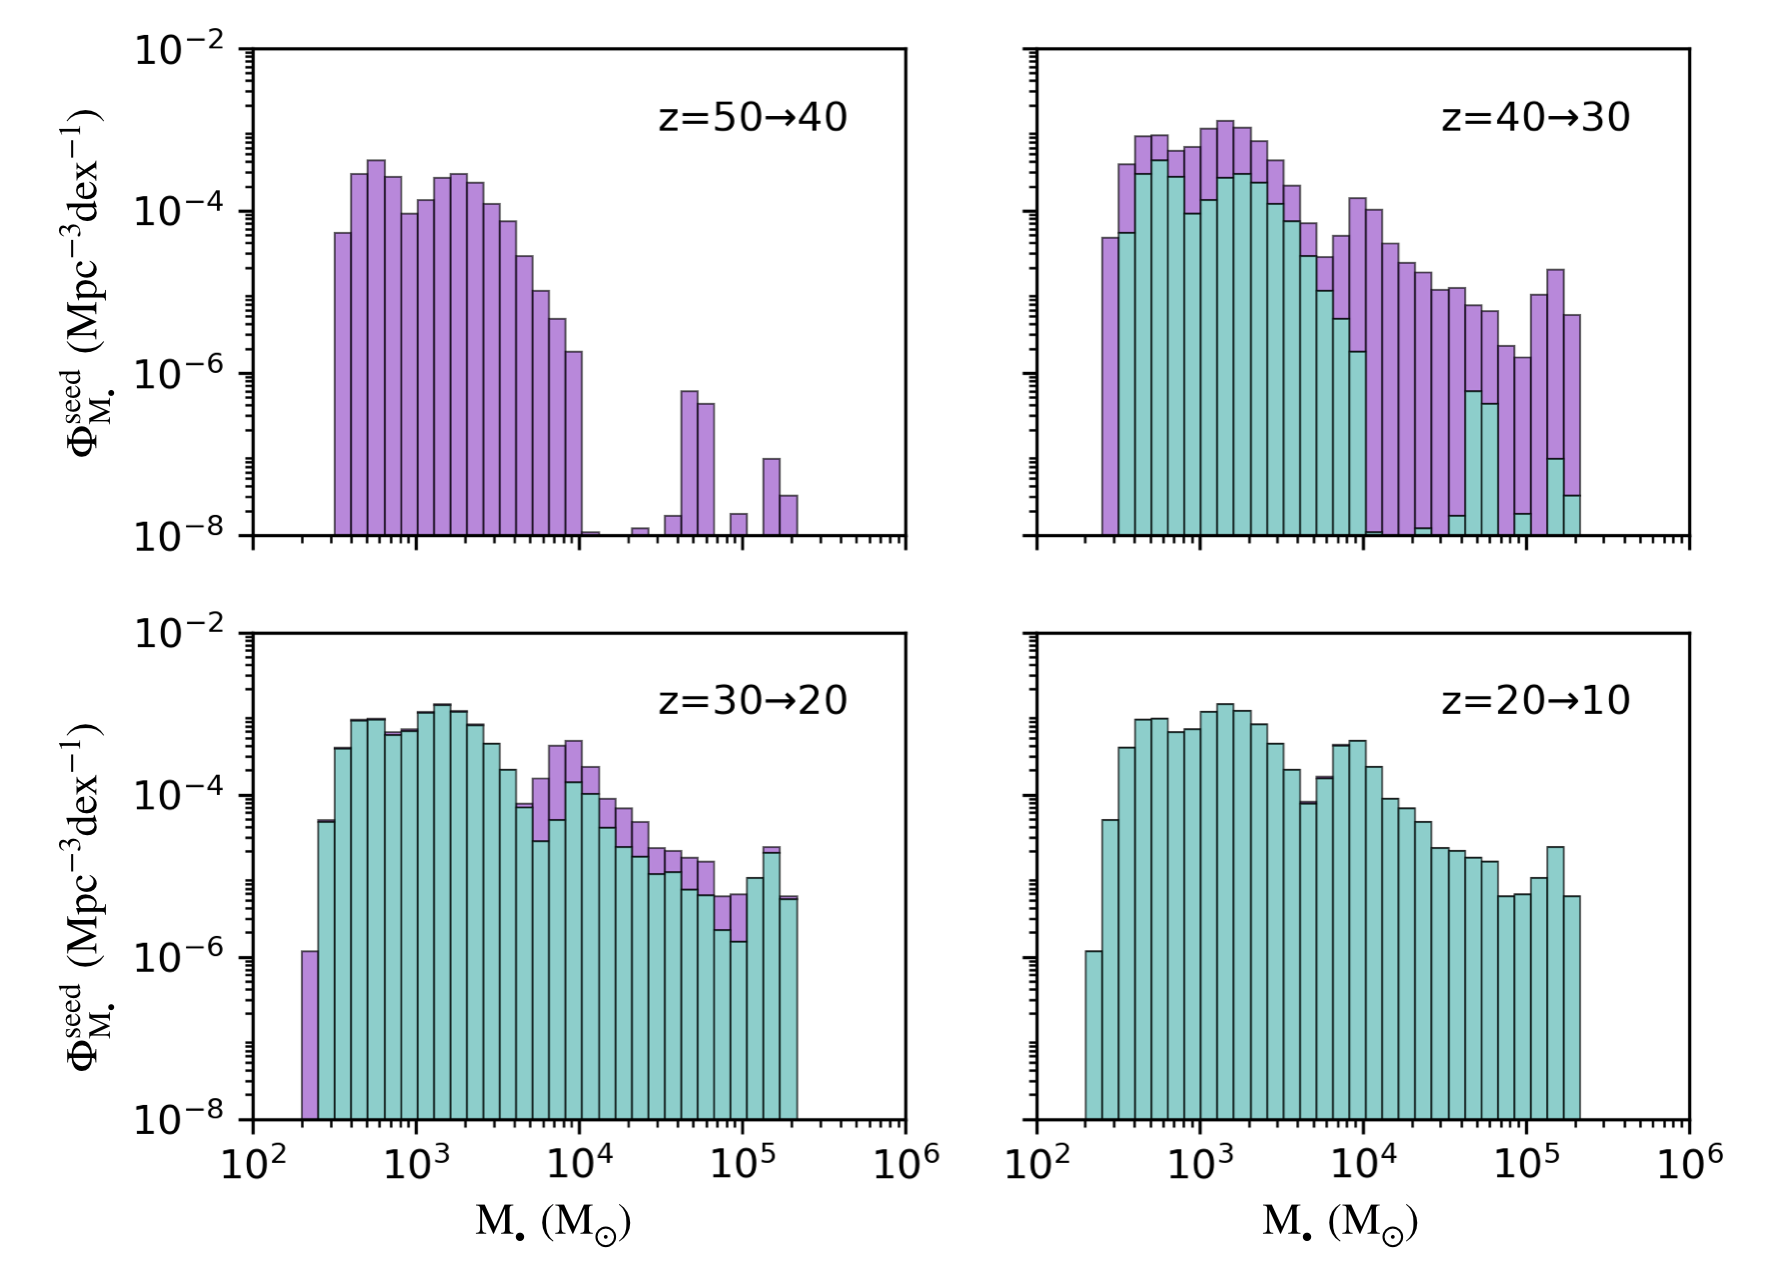
\includegraphics[width=160mm]{seedBHMF_z.png}
\caption{
Mass distribution of seed BHs formed in quasar host galaxies at different redshifts ($50\lesssim z \lesssim 10$).
%Each panel includes a redshift span of 10, 
In each panel, the cumulative number distribution of BHs formed prior than the redshift interval is shown with green bars,
and the contribution from newly-born BHs during the interval are highlighted in magenta.
%with the newly formed BHs denoted by the hatched regions, 
%and the cumulative BHs formed previously by the blue region.
The majority of seed BHs form in the epoch of $20\lesssim z \lesssim 40$.
%The most vigorous seed formation epoches are in redshift ranges $z\sim$ $40-30$ and $30-20$.
Overall, the seed BH mass distribution is extended to $M_\bullet \gtrsim 10^5~\Msun$, 
imprinted with various pathways of parent halo assembly and environmental effects as discussed in \S\ref{sec:seed}.
}
\label{fig:seedmf}
\end{figure*}


Let us consider that a seed BH with a mass of $M_{\bullet,i}$ formed in the $i$-th halo merger tree at the cosmic age 
$t_i$ ($1\leq i \leq N_{\rm tot}=10^4$),
and each of them contributes to the probability distribution function (PDF) of seed mass at a time $t$ as
% 
\begin{equation}
  p^{\rm seed}_i (\Mbh,t)\equiv \frac{\D^2 P^{\rm seed}_i}{\D \Mbh ~\D t}= \frac{ \delta(\Mbh-M_{\bullet,i})~ \delta(t-t_i)}{N_{\rm tot}}.
\end{equation}
%
Based on the cumulative seed-mass distribution of $\D P^{\rm seed}_i/ \D \Mbh$
(i.e., the integral of $p^{\rm seed}_i$ over time),
we construct the mass function from all $N_{\rm tot}$ seeds formed in one parent halo
with a mass of $\Mh$, where gas has a coherent streaming velocity of $\vbsm$ as a function of time (and redshift).
The absolute abundance of those seed BHs is calculated with the number density of the parent halo in a comoving volume at $z=6$ 
from the Sheth-Tormen mass function \citep{2001MNRAS.323....1S},
%
\begin{align}
  n_{\Mh}= \int_{\Mh}^{10\Mh}  \frac{\D n_{\mathrm{ST}}} {\D \Mh'} \D \Mh', 
\end{align}
%
where we adopt $\Mh = 10^{11}$, $10^{12}$, and $10^{13}~\Msun$, with number densities of
$n_{\Mh} = 9.9\times 10^{-4}$, $6.2\times 10^{-6}$, and $8.9\times 10^{-10}~ \text{Mpc}^{-3}$, respectively.
Combining the PDF and number density normalization, we obtain the seed BH mass function cumulative at time $t$ as
%
\begin{align}
\Phi_{\Mbh}^{\rm seed}\left(t\right) \equiv \sum_{\Mh, \vbsm} n_{\Mh} f_{\vbsm} 
\cdot \sum_{\rm itr} \frac{\D P^{\rm seed}_i}{\D \log \Mbh}\left(t\right) \Big| _{\Mh, \vbsm},
\end{align}
%
where $f_{\vbsm}$ is the volume fraction of the universe with a streaming velocity.
The value is calculated as $f_{\vbsm} = 0.6$ and $0.4$ for $\vbsm = 0$ and $\vbsm=1~\sigma_{\rm bsm}$, respectively.

Fig.~\ref{fig:seedmf} presents how the seed mass function is developed in each redshift interval.
The majority of seed BHs forms in the epoch of $20\lesssim z \lesssim 40$, and the distribution function is 
extended to $M_\bullet \gtrsim 10^5~\Msun$, imprinted with the halo assembly and environmental effects.

\orange{
Lastly, we note that in each parent halo, we consider purely the PopIII stellar remnants in the seed BH mass function construction,
neglecting the BHs formed by the second-generation PopII stars.
Formed in metal-enriched environments, PopII stellar remnants are more abundant but typically less massive.
They are likely to dominate the low mass end of the BHMF at $z\sim 6$,
thus not significantly contribute to the observable QLF and BHMF \citep{2022MNRAS.511..616T}.
}


%%%%%%%
%    Fig. 2
%%%%%%%
\begin{figure*}
\centering
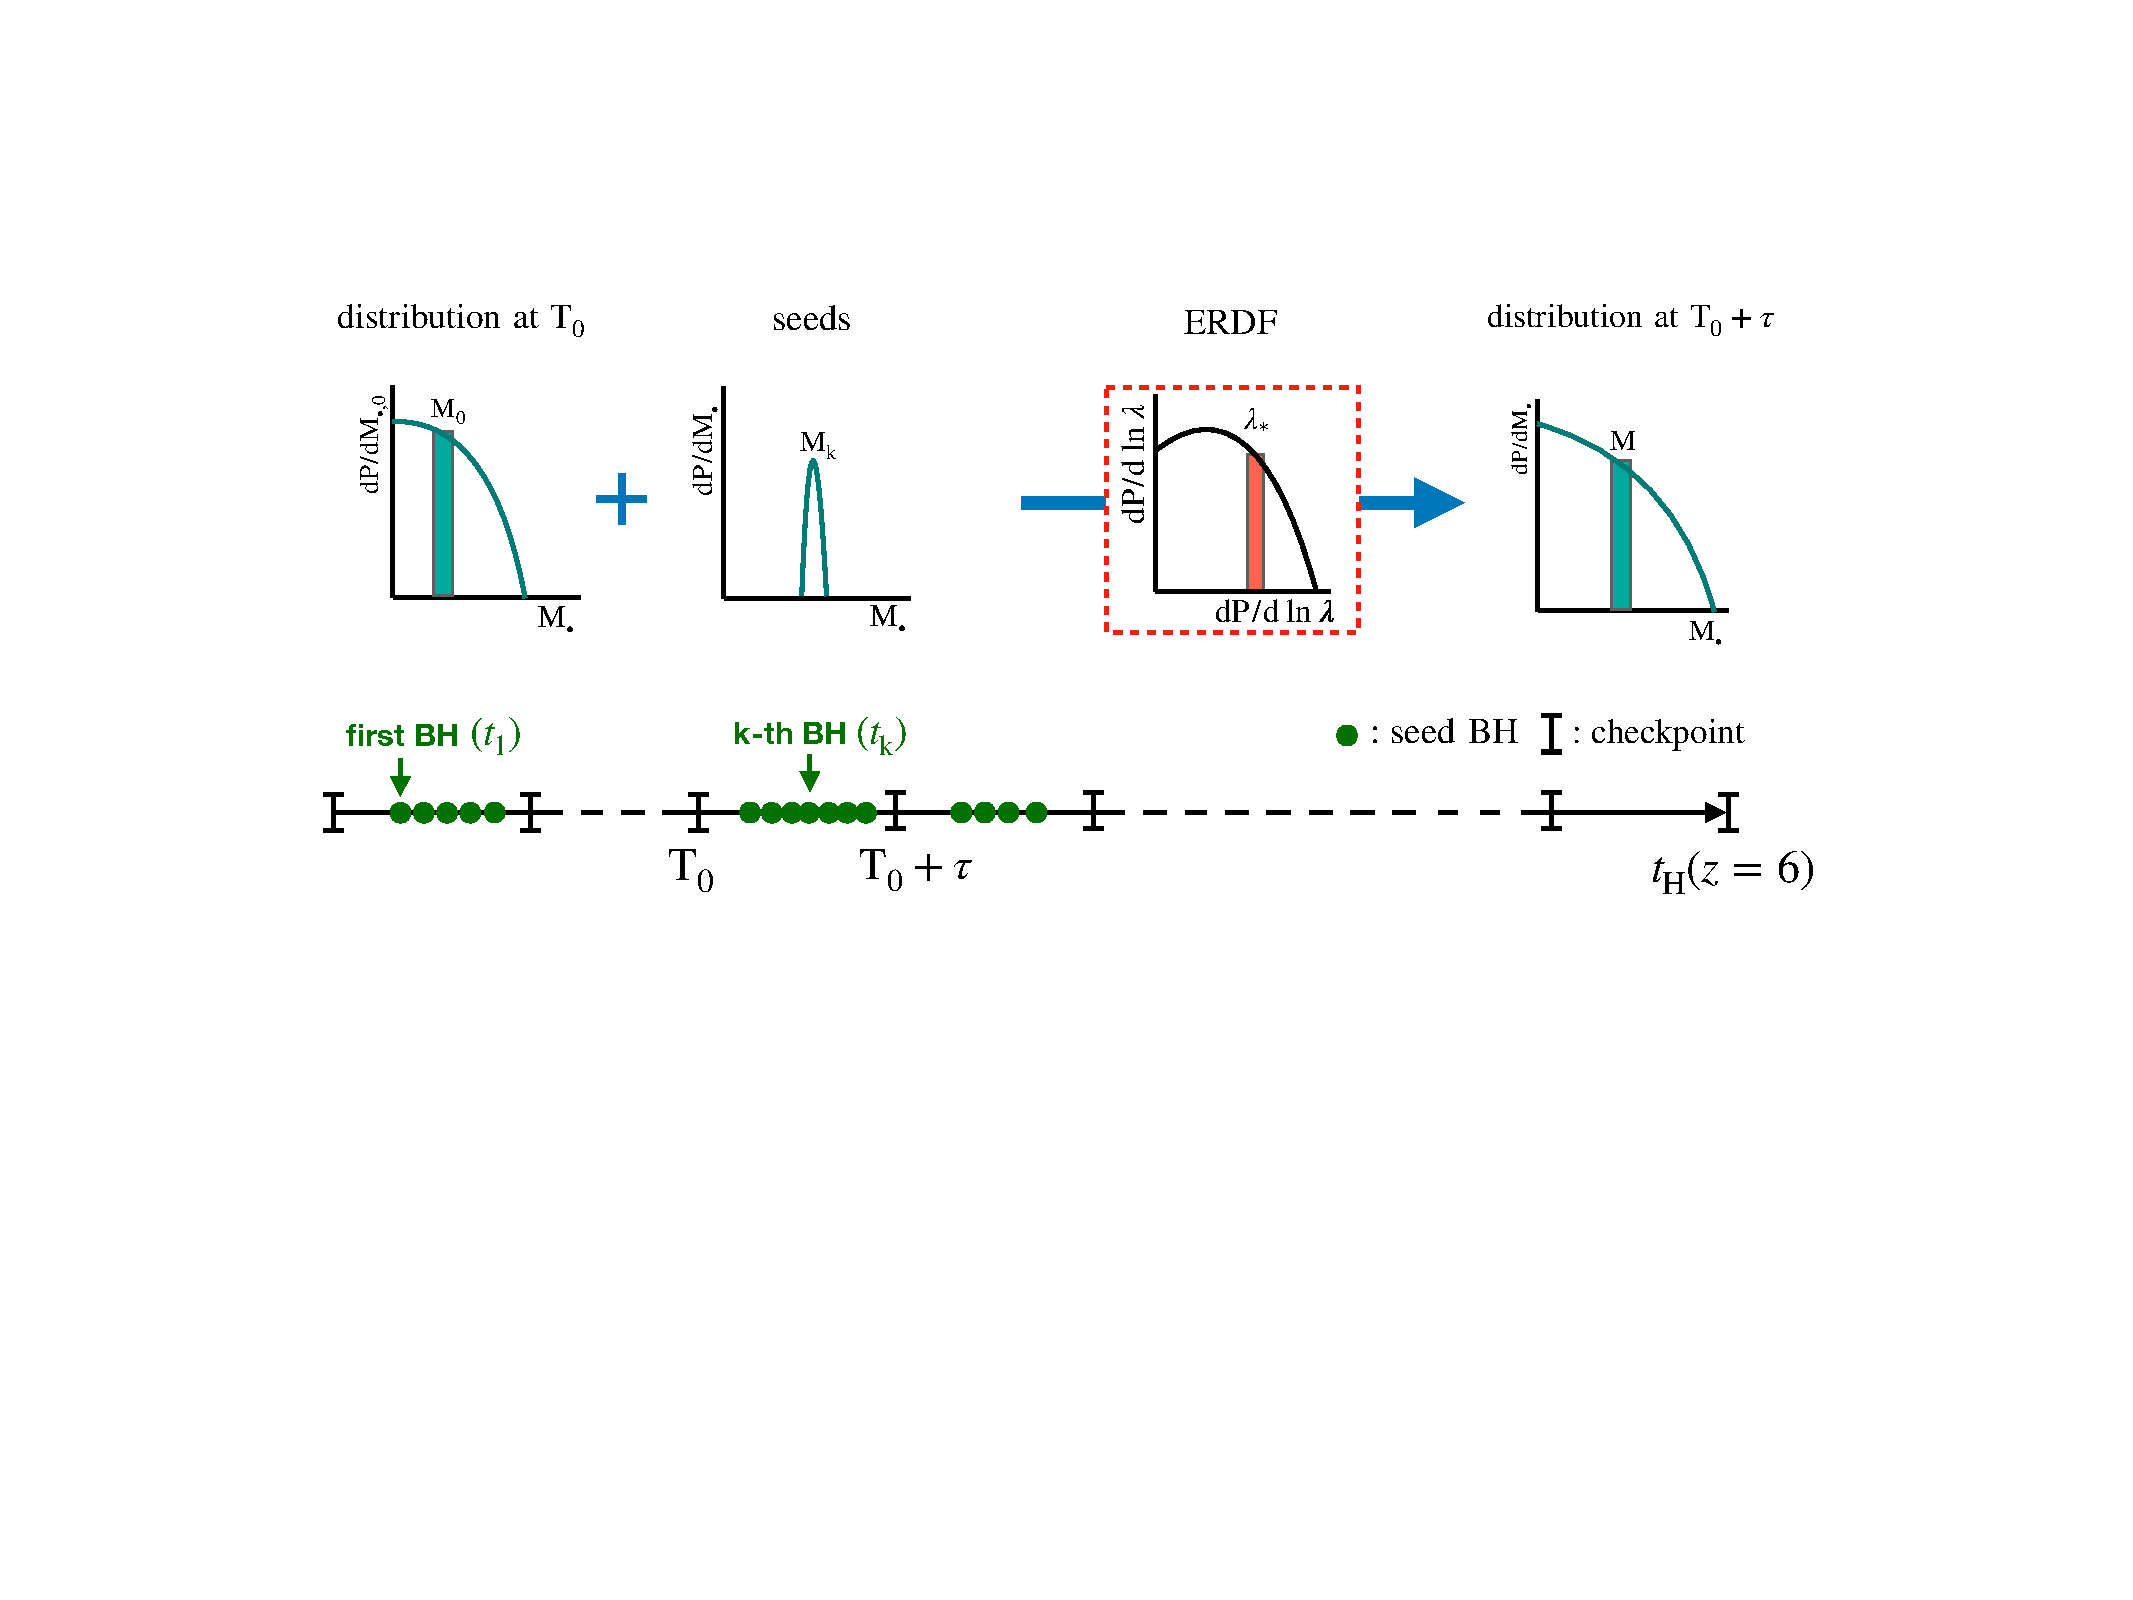
\includegraphics[width=170mm]{scheme1.pdf}
\caption{\orange{
Schematical demonstration of the procedure to calculate the evolution of BH mass distribution from the earliest BH seed to $z=6$.
The checkpoints are spaced evenly with time interval $\tau$.
From time $T_0$ to $T_0+\tau$, 
the BH mass distribution evolves with $\Delta t=\tau$.
For a newly formed seed BH $M_{\rm i}$, the probability distribution function of BH mass is a delta function, 
and the growth time is $\Delta t = T_0+\tau-t_{\rm i}$.
The probability of a BH with mass $M_0$ (or $M_{\rm i}$) to grow to $M$ after $\Delta t$ is drew from the 
ERDF following Eq.~(\ref{eq:Pl}). 
Thus the evolution of BH mass distribution is reshaped iteratively 
plus taking account of the newly formed seeds if there are any.}
}
\label{fig:scheme}
\vspace{5mm}
\end{figure*}



% Figure 1 shows the BH seeds formed in progenitors of $\Mh = 10^{11}, 10^{12}$
\vspace{2mm}



\subsection{BH mass growth}
\label{sec:model}
With BH seeds planted, we study the evolution of the BH mass distribution until $z=6$. 
The growth model of each BH is characterized by a minimal number of free parameters, 
giving the accretion rate by
%
\begin{equation}
  \label{eq:mdot}
  \Mdot_\bullet = \lambda f(\Mbh) \Mdot_\mathrm{Edd} ,
\end{equation}
where $\lambda \equiv L/L_\mathrm{Edd}$ is the luminosity-based Eddington ratio,
and $\Mdot_\mathrm{Edd} \equiv L_{\mathrm{Edd}}/\eta_0 c^2$ is the Eddington accretion rate with a radiative efficiency of $\eta_0=0.1$ \citep{1973A&A....24..337S},
which is consistent with the value obtained from the Soltan-Paczy{\'n}ski argument \citep[e.g.,][]{2002MNRAS.335..965Y,2010ApJ...725..388C}.
On the basis of studies on the mass dependence of the radiative efficiency for AGNs at $z\lesssim$ 3 
\citep{2008MNRAS.390..561C,2012ApJ...749..187L,2014ApJ...786..104U}, 
we introduce a similar functional form of
%
\begin{equation}
\label{eq:f_M}
f(\Mbh) = \frac{2}{1+\left(\Mbh /M_{\bullet,c} \right)^\delta}, 
\end{equation}
%
where $M_{\bullet,c}=10^8~\Msun$ is adopted.
\orange{
From the viewpoint of galactic-scale gas supply,
this characteristic mass is in good agreement with the critical BH mass in \citet{2021ApJ...907...74T},
above which super-Eddington mass growth of the central BHs no longer happens as
galactic scale mass supply rates into the nuclear regions cannot be as large as the Eddington rates.
}
With a positive value of $\delta$, the BH growth at the high mass end is suppressed,
while the growth speed for less masssive BHs is accelerated.
In the limit of $\delta \ll 1$, where $f(\Mbh) \simeq 1$ is nearly independent of $M_{\bullet,c}$,
the model in Eq.~(\ref{eq:f_M}) reproduces an exponential growth with an $e$-folding timescale of
$t_{\rm S} =  \Mbh/\Mdot_{\mathrm{Edd}} \approx 45$ Myr (the so-called Salpeter timescale; \citealt{1964ApJ...140..796S}).


Quasar activity is thought to take place episodically with accretion bursts triggered by gas inflows to the galactic nuclei
\citep{2005Natur.433..604D,2005ApJ...630..705H}, 
and the accretion rate declines by self-regulating feedback processes \citep[e.g.,][]{2008ApJ...686..815Y,2011ApJ...737...26N} 
or gas consumption \citep{1991MNRAS.248..754P,2005ApJ...634..901Y,2007MNRAS.377L..25K}. 
This ``flickering'' pattern of individual quasar luminosity evolution can be directly translated into the diversity 
in the Eddington ratios of quasar samples. 
We here suppose that the Eddington ratio distribution function $\D P/ \D\ln\lambda$ (ERDF) is characterized
with a Schechter function and the distribution function is independent of redshift 
\citep{2006ApJ...639..700H,2009ApJ...698.1550H}.
For type-I AGNs at low redshifts, the ERDF is characterized with a Schechter function
\citep{2015MNRAS.447.2085S,2016ApJ...826...12J,2018MNRAS.474.1225A}.
Motivated by those facts, we give the ERDF by a Schechter function with two free parameters $\lambda_0$ and $\alpha$ as
%
\begin{equation}
  \label{eq:Pl}
  \frac{\D P}{ \D \ln \lambda} \propto
  \left(\frac{\lambda} {\lambda_0} \right)^\alpha \exp{\left(-\frac{\lambda}{\lambda_0}\right)}.
\end{equation}
%
The normalization is set so that the integrant of this function over $\lambda_\mathrm{min}(=0.01) \leq \lambda < \infty$ is unity.
The minimum Eddington ratio $\lambda_\mathrm{min}$ is adopted from the simulated evolution of quasar luminosities 
that decrease mildly toward $\lambda \sim 0.1-0.01$ with $\lesssim$ 100 Myr after the peak activity \citep{2011ApJ...737...26N}.
Moreover, a turnover in the ERDF at the lowest value of $\lambda\lesssim 0.01-0.001$ is suggested by observations \citep{2018MNRAS.474.1225A}.  


To characterize the ERDF for a BH population at any time snapshot together with episodic 
accretion patterns of individual BHs, 
we introduce a time duration of $\tlife$, during which a single value of $\lambda$ is assigned to an accreting BH
following the ERDF of Eq.~(\ref{eq:Pl}).
In this way, we give a different growth speed of a BH in every period with a duration of $\tlife$ until $z=6$ 
(the corresponding cosmic age is $t_{\rm H}\gtrsim 900$ Myr).
This treatment enables us to capture the nature of accretion bursts and prohibit an unrealistically 
long-lasting rapid growth phase of a BH.
This phenomenological method also avoids numerous uncertainties in modeling of the galaxy assembly, 
gas feeding, and BH feedback processes in the quasar progenitor halos.
Instead of treating those ingredients implemented in previous semi-analytical models, we extract 
an averaged but fundamental timescale that governs mutual correlation between the QLF and BHMF,
based on direct comparison to those distribution functions for observed high-$z$ quasar population.


Thus far, we assume that {\it all} the seed BHs formed in parent halos participate in the assembly of SMBHs and 
end up in quasar host galaxies by $z\simeq 6$.
To relax this stringent assumption, we introduce the seeding fraction of $\fseed (\leq 1)$.
As discussed in \citet{2009ApJ...696.1798T}, a small value of $\fseed <1$ is required to avoid overproduction of SMBHs at $z\sim 6$,
depending on BH seeding and growth mechanisms in semi-analytical models.
Since the value has been poorly constrained both by theoretical and observational studies, we treat it as a free parameter.
We take three different values of $\fseed = 1$, $0.1$, and $0.01$, and explore its effect on producing the QLF and BHMF.
Since we find that the results in the cases of $\fseed = 1$ and $0.1$ are overall similar,
we thus show only the cases with $\fseed=0.1$ and $0.01$ in the following discussion.
Note that the seed mass function shown in Fig.~\ref{fig:seedmf} is given with $\fseed = 1$.



\subsection{BH mass function}\label{sec:MF}

We describe how to calculate the time evolution of the BH mass function, 
combining the semi-analytical growth model and ERDF (see Eqs.~\ref{eq:mdot} and \ref{eq:Pl}).
The schematic illustration of our numerical procedure is shown in Fig.~\ref{fig:scheme}. 
We first set a series of checkpoints with an interval of $\tlife$, 
tracing back from $t_{\rm H}(z=6)$ to just prior than the first seed formation time $t_1$, where $t_i$ is the $i$-th seed forming time
as defined in \S\ref{sec:seed} ($1\leq i\leq N_{\rm tot}$).
Note that the number of the checkpoints is given by $\lceil (t_{\rm H}-t_1)/\tau \rceil+1$, where $\lceil x\rceil \equiv {\rm min}\{n \in \mathbb{Z}~ |~x\leq n\}$.


The time evolution of the BH mass distribution is calculated from the first checkpoint to $t_{\rm H}(z=6)$ by adding newly-forming seed BHs
and taking into account growth of existing BHs via mass accretion.
For a given mass distribution function $\D P/\D  M_{\bullet, 0}$ at a checkpoint of $t=T_0$, 
we give its evolution at $t=T_0+\Delta t$ as
%
\begin{equation}
  \label{eq:dpdm}
  \frac{\D P}{\D \Mbh} = \int
   \frac{\D P}{\D \ln \lambda}\Big|_{\lambda_\ast} \cdot
   \frac{\D \ln \lambda_\ast}{\D  \Mbh}\Big|_{\Delta t, M_{\bullet,0}} \cdot
  \frac{\D P}{\D M_{\bullet, 0}}~\D M_{\bullet, 0},
\end{equation}
%
where $\lambda_\ast$ is the Eddington ratio required for a BH with $M_{\bullet,0}$ to grow up to $\Mbh$ within $\Delta t$
and is calculated analytically from Eq.~(\ref{eq:mdot}) by
%
\begin{equation}
  \label{eq:mi2m}
\frac{2 \lambda_\ast \Delta t}{t_{\rm S}}=
  \ln \left(\frac{\Mbh} {M_{\bullet,i}}\right) + \frac{1}{\delta} 
  \left[ \left(\frac{\Mbh}{M_{\bullet,c}}\right)^\delta - \left(\frac{M_{\bullet, 0}}{M_{\bullet,c}}\right)^\delta \right],
\end{equation}
%
and the derivative of ($\D \ln \lambda_\ast / \D  \Mbh )|_{\Delta t, M_{\bullet,0}}$ is also determined.
For existing BHs formed prior to this checkpoint, we calculate the evolution of the mass distribution by setting $\Delta t = \tlife$.
For a seed BH formed during this cycle (i.e., $T_0\leq t_k < T_0+\tlife$), 
we evolve $\D P^{\rm seed}_k/\D \Mbh$ by setting $\Delta t = T_0+\tlife -t_k$ and add it to the mass distribution 
of the existing BHs at $t=T_0+\tlife$.
Combining the PDF and number density normalization, the BHMF is given by
%
\begin{equation}
  \Phi_{\Mbh} 
  =\sum_{\Mh, \vbsm} n_{\Mh} f_{\vbsm} {\fseed} \cdot \frac{\D P}{\D \log \Mbh}\Big|_{\Mh, \vbsm}.
 \end{equation}


To follow the time evolution of the mass function, we set up 
logarithmically spaced mass grids at $10^2 \leq \Mbh /\Msun \leq 10^{12}$.
The number of the grid points is set to $N_{\rm bin}=800$, so that the convergence of the numerical result is ensured.
Our result of $\Phi_{\Mbh}$ is consistent with that obtained from the direct sampling method, where 
we consider the growth of $10^7$ individual BHs rather than the evolution of smooth analytical mass distribution functions.
Our method reduces the statistical errors seen in the direct sampling method 
and thus allows us to extend the BHMF and QLF to the higher mass and brighter end
in a reasonable computational time.



\vspace{2mm}
\subsection{Obscuration-corrected QLF}\label{sec:LF}

Using the BHMF and its evolution, we construct the QLF, which can be directly probed by high-$z$ quasar observations.
For an accreting BH with a bolometric luminosity of $\Lbol=\lambda L_\mathrm{Edd}$, 
its rest-frame ultraviolot (UV) absolute magnitude of $\Muv$ at 1450 $\mathrm{\AA}$ is estimated by
%
\begin{equation}
  \label{eq:M1450}
  \Muv= -21.0-2.5 \log  \left(\frac{\Lbol}{10^{45}~\mathrm{erg~s}^{-1}} \right) ~[\rm{mag}],
\end{equation}
%
where a bolometric correction factor of $f^{\rm bol}_{1450}=4.4$ for the monochromatic UV band is adopted
\citep{2006ApJS..166..470R}.
We construct the QLF from the BHMF, combining this conversion factor and ERDF.
However, we note that the shape and normalization of the {\it intrinsic} QLF is not necessary identical to the {\it observed} QLF
because quasar surveys with optical and near-infrared telescopes are not sensitive to the obscured quasar population at high redshifts,
i.e., the number of fainter quasars observed as type-I AGNs is largely reduced by the obscuration effect
\citep{2003ApJ...598..886U,2007A&A...463...79G,2008A&A...490..905H,2014ApJ...786..104U,2014MNRAS.437.3550M}. 


% obs fraction 
A widely-accepted mechanism causing quasar obscuration is extinction by dusty tori and dense gas clouds 
in the circumnuclear region, hence tightly related with gas fueling and feedback processes from accreting BHs 
\citep[see][for a review]{2018ARA&A..56..625H}.
In addition, dense gas clouds at galactic larger scales may have a significant contribution to quasar obscuration at 
higher redshifts \citep{2020MNRAS.495.2135N}.
%and the obscured fraction is expected to increase with redshift \citep[]{2022arXiv220603508G}. 
%However, we adopt the prescription of the obscured fraction constrained from quasar observations at $z\lesssim 5$ 
However, the physical origin and conditions for high-z quasar obscuration has been poorly understood yet.
Observationally, the obscured fraction of AGNs with hydrogen column density of $N_{\rm H}>10^{22}~{\rm cm}^{-2}$
can be estimated from spectral analyses in the X-ray band
\citep[e.g.,][]{2003ApJ...598..886U,2007A&A...463...79G,2008A&A...490..905H}. 
The obscured fraction is nearly $\gtrsim 80\%$ at $L_{\rm X}<10^{43}~{\rm erg~s}^{-1}$ and 
decreases with the X-ray luminosity \citep{2014ApJ...786..104U,2014MNRAS.437.3550M}.
The exact function shape still remains under debate, but the overall dependence on the X-ray luminosity holds.
Moreover, the obscured fraction is found to increase gradually toward higher redshifts and is saturated at $z\gtrsim 2-3$
\citep{2008A&A...490..905H,2014ApJ...786..104U,2014MNRAS.437.3550M,2018MNRAS.473.2378V,2022arXiv220603508G}.


In this study, we adopt the obscuration fraction $\fobsc$ given by \cite{2014ApJ...786..104U} as
%
\begin{equation}
\fobsc = \text{min}\left\{0.84 , 11.23-0.24 \log \left(\frac{\Lbol}{L_\odot}\right) \right \}.
%  \fobsc = \text{min}\lbrace  0.84 , 0.73-0.24\times[ \log (\Lbol/L_\odot) -43.75] \rbrace,
\end{equation}
%
Here, we use the bolometric correction factor from the hard X-ray band 
%
\begin{equation}
  f^{\rm bol}_{\rm X} =
  a\left[1+\left(\frac{\log \left(\Lbol / L_\odot\right)}{b}\right)^{c}\right],
\end{equation}
%
where $a=10.96$, $b = 11.93$, and $c = 17.79$ are given in Eq.~(2) of \citet{2020A&A...636A..73D}. 
In our analysis, we neglect the contribution from Compton-thick AGNs with $N_\mathrm{H}>10^{24}$ cm$^{-2}$, 
which are obscured even in the hard X-ray band and show possible dependence on quasar properties.
It is worth noting that the obscured fraction for high-$z$ quasar populations is still under investigation.
%and the uncertainties would affect our analyses for fainter quasars.
We leave more comprehensive arguments about the quasar obscuration effect for future work.


After taking into account the obscuration effect, 
the observed QLF for a given BHMF and ERDF is calculated as
%
\begin{equation}
\label{eq:dn_dM1450}
\Phi_{\Muv} 
%\equiv \frac{\D n}{\D \Muv} \nonumber \\
 = (1 -\fobsc)  % \nonumber \\
\int \frac{\D P}{\D \ln \lambda}\Big|_{\tilde{\lambda}}  \cdot
\frac{\D \ln \tilde{\lambda}}{\D \Muv} \cdot
 \Phi_{\Mbh} \D \log \Mbh,
\end{equation}
%
where the values of $\tilde{\lambda}=\lambda(\Muv, \Mbh)$ and $\D \ln \tilde{\lambda}/\D \Muv$ are calculated analytically from Eq.~(\ref{eq:M1450}).
%
Hence, the observed QLF can be produced simultaneously with the BHMF from a set of model parameters, 
to be compared with the ones from observation.




\vspace{2mm}
\subsection{MCMC fitting}\label{sec:fitting}



In this section, we describe the MCMC fitting procedure used to optimize 
the BH growth parameters so that the observed BHMF and QLF are consistently reproduced. 
As discussed in Section~\ref{sec:MF}, we consider five parameters of $\tlife$, $\delta$, $\alpha$, $\lambda_0$, and $\fseed$.
The best-fit values of the first four parameters are calculated by the MCMC method, while $\fseed$ is fixed to a single value.
% In what follows, we describe the results for $\fseed = 0.1$ and $0.01$ (see Appendix for the case with $\fseed =1.0$).

% prior
In this analysis, we constrain those parameters to be within certain physically acceptable ranges, 
assuming a prior function for each quantity.
We use a uniform prior on $\tlife$ with a limit of $10~{\rm Myr} \leq \tlife \leq 200~{\rm Myr}$,
motivated by the constraints on the quasar lifetime based on various observations
\citep[e.g.,][]{2004cbhg.symp..169M}.
The parameter of $\delta$ that characterizes a non-exponential BH growth 
is constrained at $\log \delta$ from $-4$ to $-0.3$
\footnote[3]{ We first set a uniform prior at $0\leq \delta \leq 1$, 
and find the posterior distribution assembles to $\delta \lesssim 0.1$.
We then switch to impose the $\log \delta$ prior to improve the fitting performance at small $\delta$ values.}.
The prior function is uniform at $\log \delta \geq -3$ and is imposed to decay with an exponential cutoff at $\log \delta < -3$,
which is small enough for the model to be approximately mass independent, i.e., $f(M_\bullet)\simeq1$.
For the characteristic Eddington ratio $\lambda_0$ in the Schechter-type ERDF, 
we impose a Gaussian prior function with a mean value of $\mu_{\lambda_0}=0.6$ and a dispersion of $\sigma_{\lambda_0}=0.4$.
The choice is motivated by the brightest quasar samples at $z=$ 6, whose ERDF is peaked around $\lambda \sim 0.6$ 
% \citep[e.g.,][Onoue et al. in preparation]{2010AJ....140..546W}.
after luminosity bias correction \citep[e.g.,][]{2010AJ....140..546W}.
For the low-$\lambda$ slope of $\alpha$ in the ERDF, we assign a Gaussian prior function with a mean value 
$\mu_{\alpha}=0$ and a dispersion of $\sigma_{\alpha}=0.3$.
Note that the value of $\alpha$ remains poorly constrained by the current high-$z$ quasar observations,
but the low-$z$ quasar samples support $-0.3 \lesssim \alpha \lesssim 0.3$ \citep[e.g., see Figure 21 in][]{2015MNRAS.447.2085S}.


The observed BHMF data is taken from \citet{2010AJ....140..546W} (hereafter, \citetalias{2010AJ....140..546W}), where 
the virial BH mass measurements for 17 bright quasars at $z\simeq $ 6 are used.
Although the BHMF spans over $10^7 < \Mbh/\Msun <10^{10}$, the best constraint is given around 
$\Mbh \simeq 10^{8.5}~\Msun$
and thus the statistical error size becomes larger both at the lower and higher mass range.
We set up 10 logarithmically spaced mass bins and adopt errors with sizes increasing quadratically as 
$\Phi_{\Mbh}^{\rm err} = \pm \{0.2 +   [\log (\Mbh/10^{8.5}~\Msun)]^2/3 \}~{\rm dex}$,
covering the same mass range as in their bootstrap resamples (see Figure 8 of W10). 
The observed QLF is taken from \citet{2018ApJ...869..150M} (hereafter \citetalias{2018ApJ...869..150M}) 
over a wide range of $-30 < \Muv <-22$ mag (see their Table 4 and Figure 13). 
The magnitude bins and the error sizes are given consistently with \citetalias{2018ApJ...869..150M}.

  

% posterior
Following the prior distribution functions, the four parameters are sampled to generate the synthetic 
BHMF and QLF dataset, which are compared to the observational dataset. 
The discrepancy between the model and observational data is evaluated with a $\chi^2$-value defined by
%
\begin{align}
  \chi^2 = \sum_{x,i}
  \frac{\left(\log{\Phi^{\rm mod}_{x,i}} - \log{\Phi^{\rm obs}_{x,i}}\right)^2}{(\log{\Phi^{\rm err}_{x,i}})^2},
\end{align}
%
where $\Phi^{\rm mod}_{x,i}$ and $\Phi^{\rm obs}_{x,i}$ represent the modeled and observational value 
on the \textit{i-}th bin of the BHMF ($x=\Mbh$) and QLF ($x=\Muv$), and $\Phi^{\rm err}_{x,i}$ is the corresponding error.
Adopting 10 mass bins and 12 magnitude bins, we treat the errors from comparison both in the BHMF and QLF
with a nearly equal weight.
The posterior distribution of the MCMC fitting is stabilized around the minimum value of $\chi^2$ (highest likelihood), 
with the models best reproducing the $z=$ 6 BHMF and QLF.



\vspace{2mm}
%\section{Results}\label{sec:result}
\section{Results}\label{sec:fitting_result}


%\vspace{2mm}
%\subsection{Fitting Results}\label{sec:fitting_result}


%%%%%%%
%    Fig. 3
%%%%%%%
\begin{figure*}
\centering
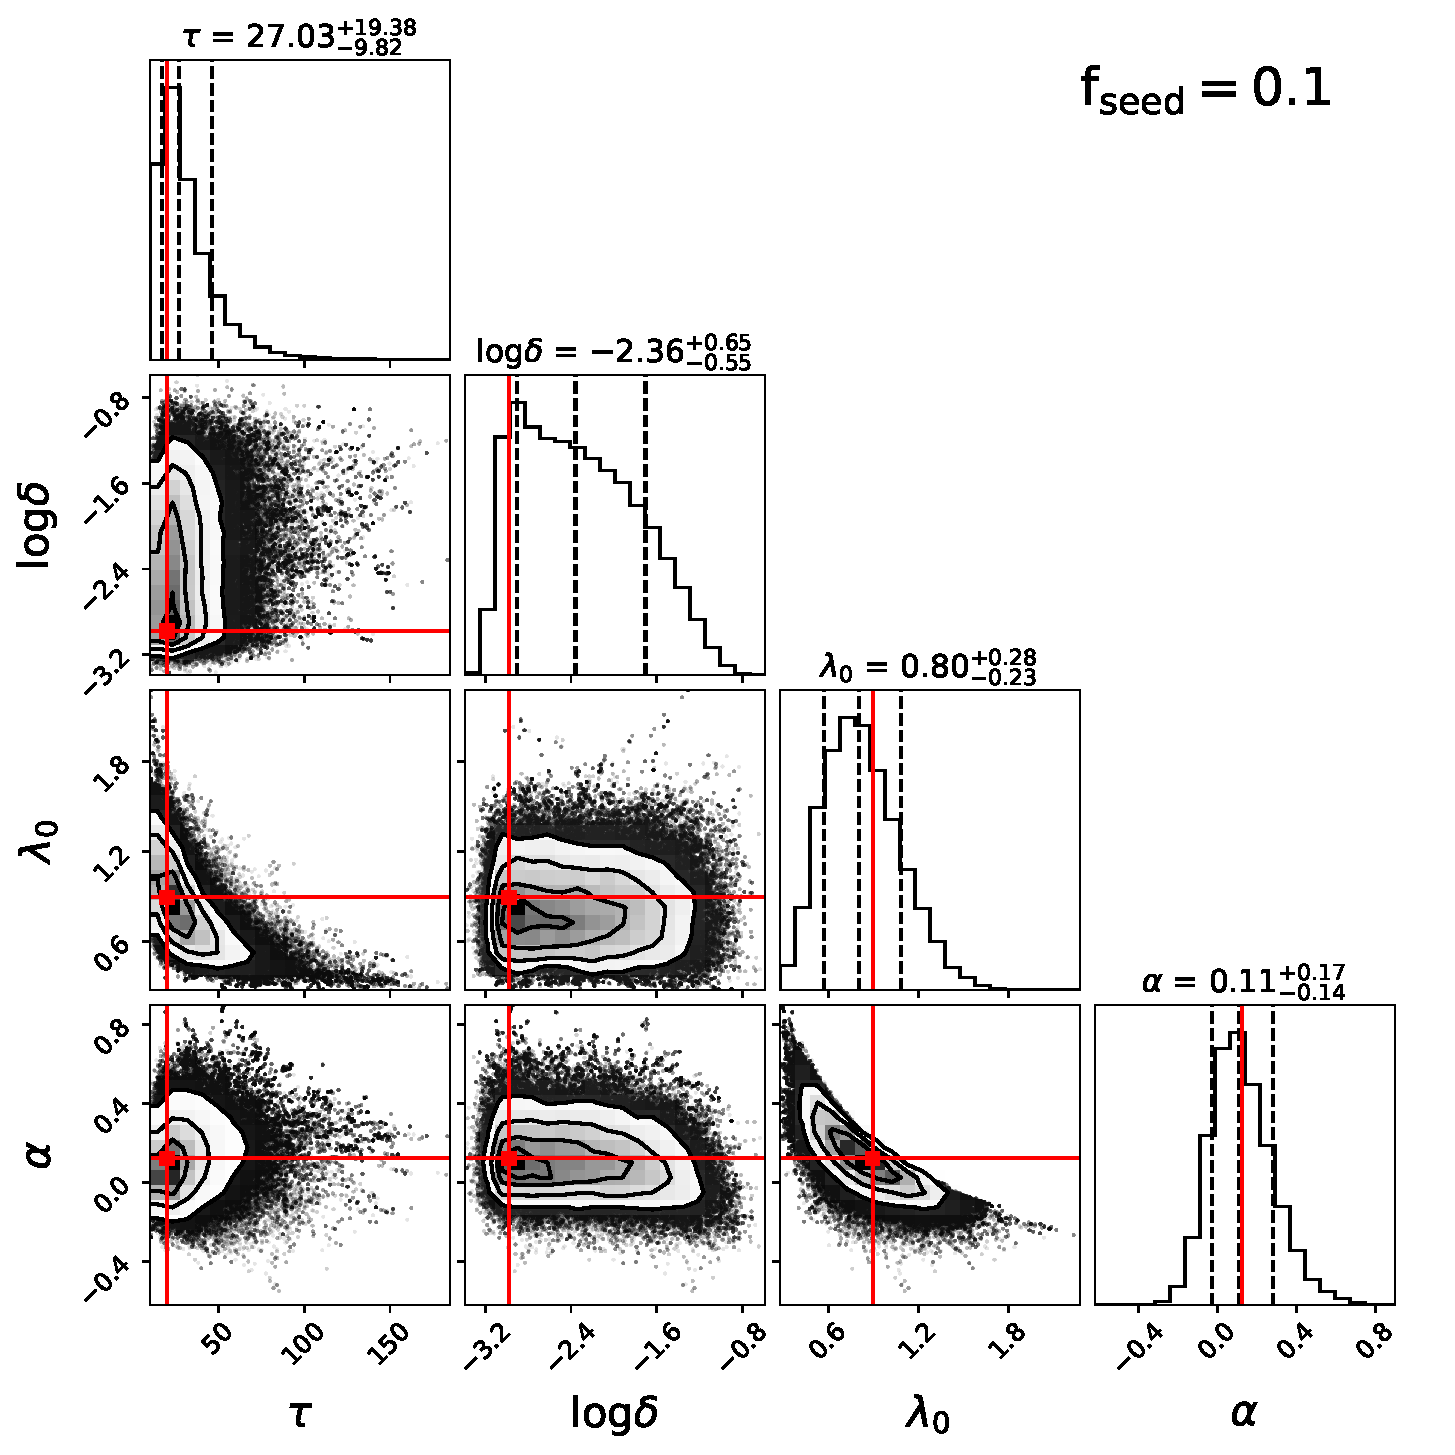
\includegraphics[width=85mm]{f1_corner.pdf}
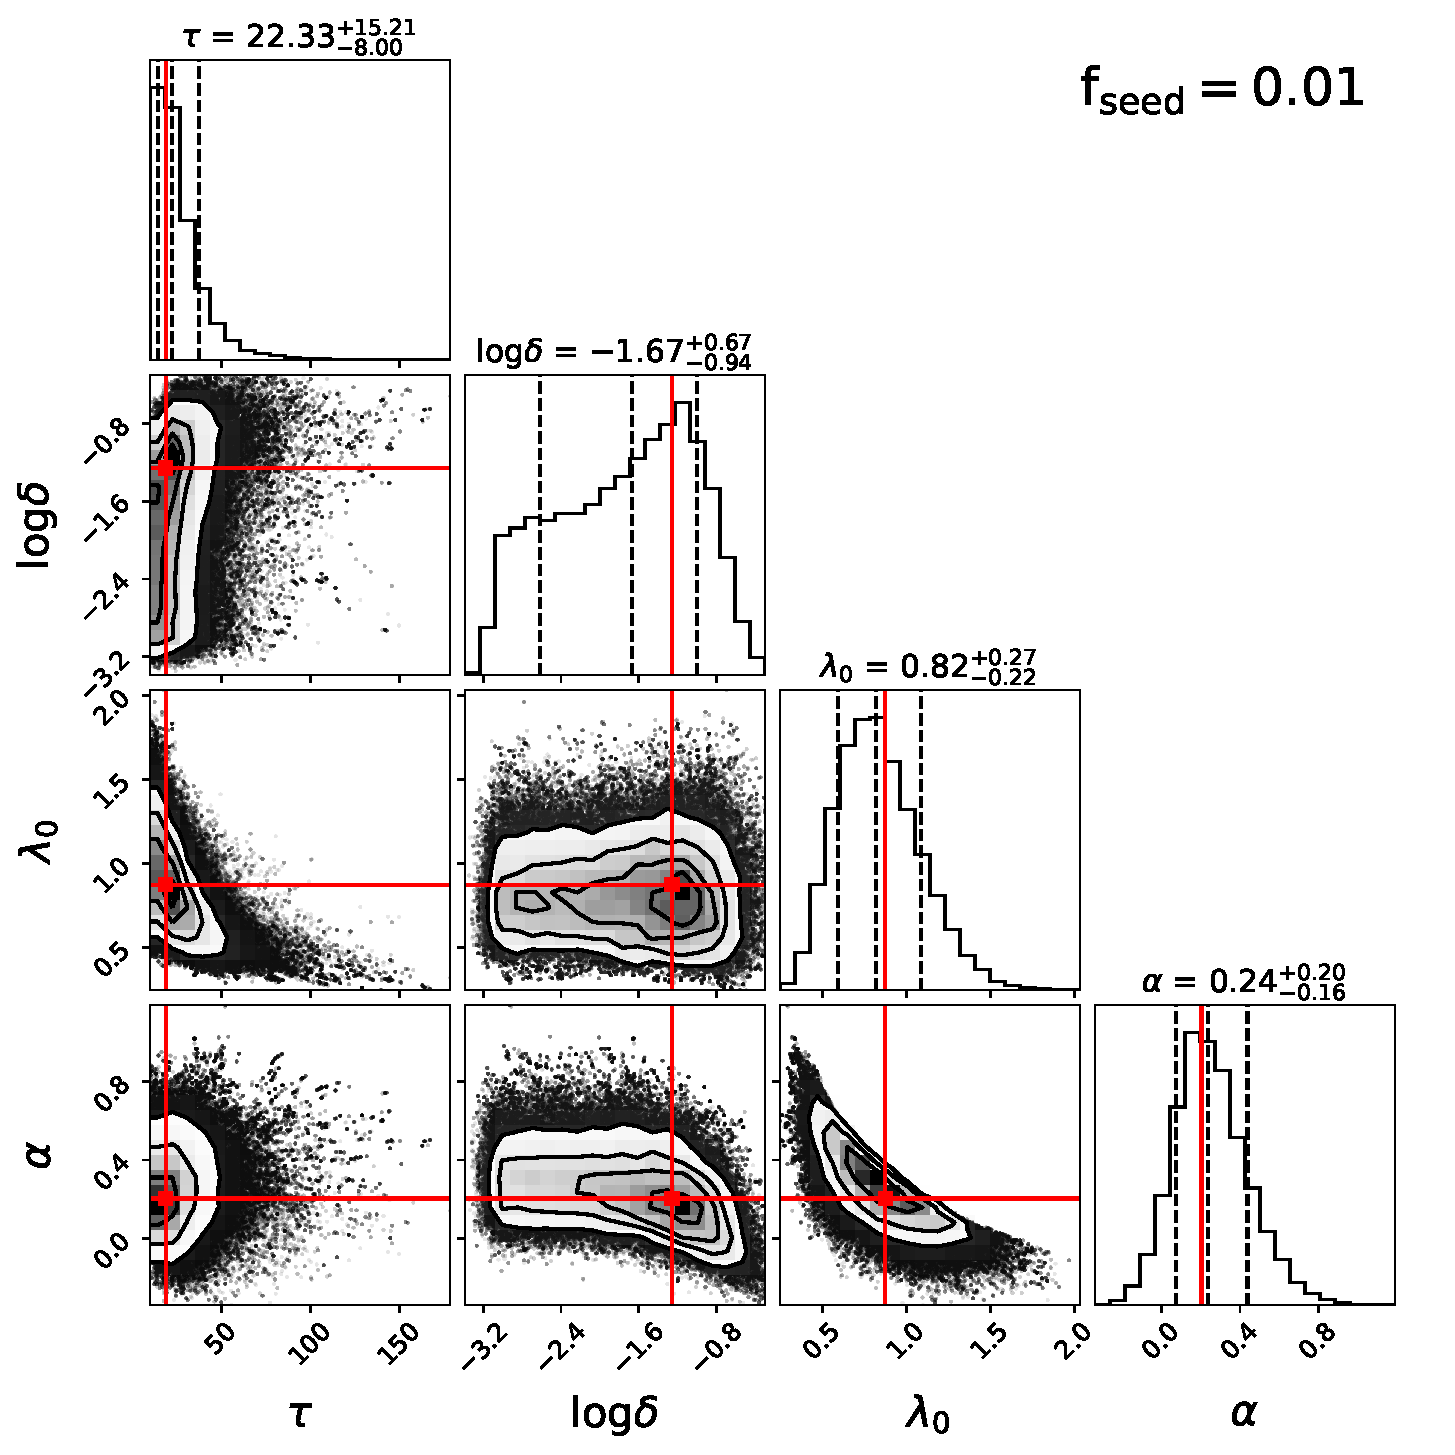
\includegraphics[width=85mm]{f2_corner.pdf}
\caption{
Two dimensional posterior distribution of all the model parameters with $\fseed=0.1$ and 0.01, 
along with the marginalized one dimensional projection.
% and the two dimensional distribution between every two parameters. 
The distribution of three parameters ($\tau$, $\lambda_0$, and $\alpha$) show single peaks,
displaying the convergence of those parameters.
The distribution of $\log\delta$ is relatively broader but suggests that the value of $\delta$
is sufficiently low and thus the mass-dependent growth model is excluded.
}
\label{fig:contour}
\vspace{5mm}
\end{figure*}
%


We discuss the MCMC fitting results and compare the BHMF and QLF with those observed distribution functions.
In Fig.~\ref{fig:contour}, we visualize the fitting results for each parameter in two-dimensional 
posterior distribution for the case of $\fseed= 0.1$ (left) and $0.01$ (right), respectively.
The three vertical dashed lines in the one-dimensional posterior distribution of each parameter
correspond to 16\%, 50\%, and 84\% quantiles in the cumulative distribution, respectively.
The best-fit values shown with the red lines are listed in Table~\ref{tab:best_fits},
displaying consistency with the peaks in the one-dimensional distribution.
%Note that the best-fit values may not overlap the 50\% quantile lines,
%and the deviation are significant in asymmetric one-dimensional distribution.


For the two cases, the best-fit solution consistently shows a small value of $\delta < 0.1$.
This result favors the nearly exponential BH growth model with minor mass dependence (Eqs.~\ref{eq:mdot} and \ref{eq:f_M}).
The typical duration of quasar activity is required to be $\tlife \simeq 20-30$ Myr for both the cases.
This suggests that accreting seed BHs vary their growth speeds and their Eddington ratios 
$\simeq 30-40$ times on average toward the cosmic time at $z\simeq 6$.
The timescale of $\tlife$ is also related to the quasar lifetimes of $t_{\rm Q}\sim 1-10$ Myr, 
which are estimated by the measurement of the physical extents of hydrogen Ly$\alpha$ proximity zones 
observed in the rest-frame UV spectra \citep[e.g.,][]{2018ApJ...867...30E,2019ApJ...884L..19D}.
More detailed comparison is discussed in \S\ref{sec:evol}.

%%%%%%%
%    Table. 1
%%%%%%%
\begin{deluxetable}{lcccccc}%[t!]
\tablecolumns{1}
\renewcommand\thetable{1} %! fix indexing
\tablewidth{0pt}
\tablecaption{Best-fit Parameters \label{tab:best_fits}} %!!!!
\tablehead{
  \colhead{$\fseed$}  & \colhead{$\tau$ (Myr)} & \colhead{$\delta$} &  \colhead{$\lambda_0$}  & \colhead{$\alpha$}  & \colhead{$\chi^2$}
}
\startdata
1.0    &  23.13 &    0.001    &   0.96    &   -0.06    &    15.77   \\
0.1    &  20.07 &    0.001    &   0.89    &    0.12    &    8.27    \\
0.01   &  18.76 &    0.055    &   0.87    &    0.20    &    6.21    \\
\enddata
\tablecomments{
The best-fit parameters optimized by MCMC sampling for different cases of $\fseed$.
The fitting performance is characterized by the relative magnitudes of the $\chi^2$ value.% (see Eq.~\ref{eq:chi2}).
}
\end{deluxetable}


The best-fit parameters for the two cases of $\fseed$ reproduce the bulk properties of the BHMF and QLF at $z\sim 6$,
despite the ten-fold difference in the seeding fraction.
%The two parameters characterizing the ERDF are given as
%$(\lambda_0,\alpha) = (0.89,0.12)$ and $(0.87,0.20)$ for $\fseed=0.1$ and $0.01$, respectively.
With the fitted values for the ERDF, the fraction of super-Eddington accreting BHs is estimated as 
$P(\lambda \geq 1)=0.064$ and $0.075$ for $\fseed=0.1$ and $0.01$, respectively.
While the probability of rapid accretion in each cycle differs slightly between the two cases,
multiple accretion episodes enlarge the difference and accelerate BH growth for the lower seeding fraction.
Moreover, the case with $\fseed=0.01$ requires a higher value of $\delta (\simeq 0.055)$,
promoting the growth of less massive BHs with $M_\bullet <10^8~\Msun$.
Therefore, a larger fraction of seed BHs are delivered into the SMBH regime,
and the ten-fold difference in $\fseed$ is nearly compensated.
The characteristic Eddington ratio needs to be close to unity, otherwise the highest luminosity and BH mass
in the model would differ from those in observations.
On the other hand, the power-law index of $\alpha$ in the ERDF increases as the seeding fraction decreases,
indicating that the fraction of active BHs with $\lambda \gtrsim 1$ is elevated. 
Thus, with lower seeding fractions, the high-$z$ quasar assembly ought to experience more active growth phases to reproduce the observations.

%%%%%%%
%    Fig. 4
%%%%%%%
\begin{figure*}
\centering
%\includegraphics[width=170mm]{fits_MF.png}
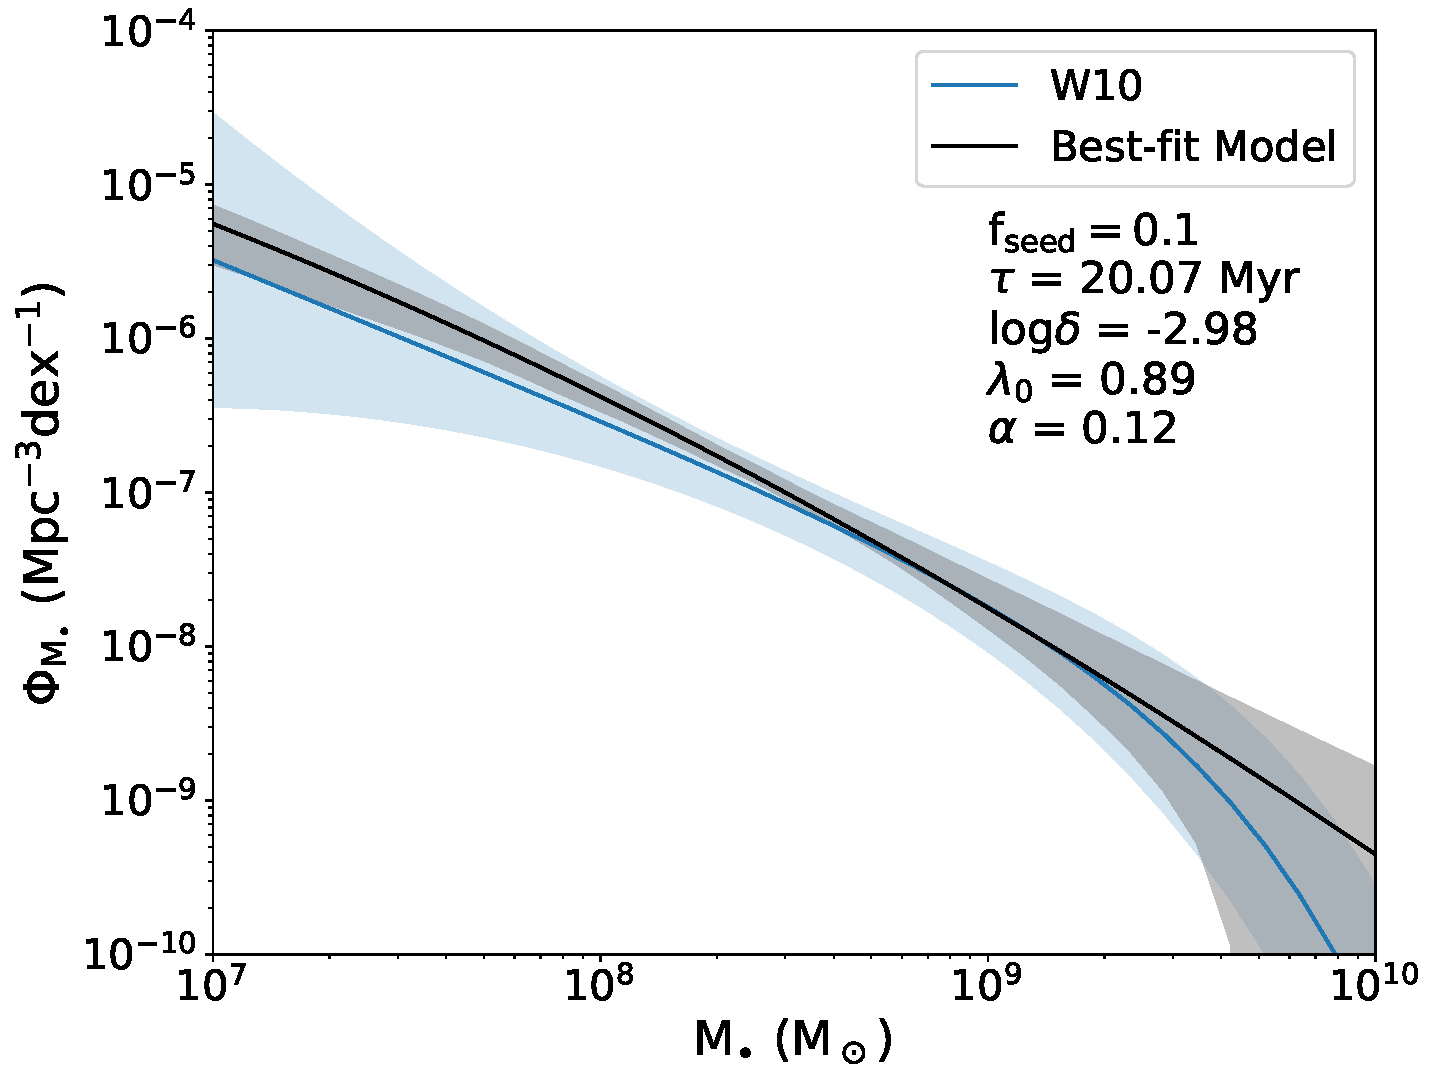
\includegraphics[width=85mm]{f1ndraw60MF_spread.pdf}\hspace{3mm}
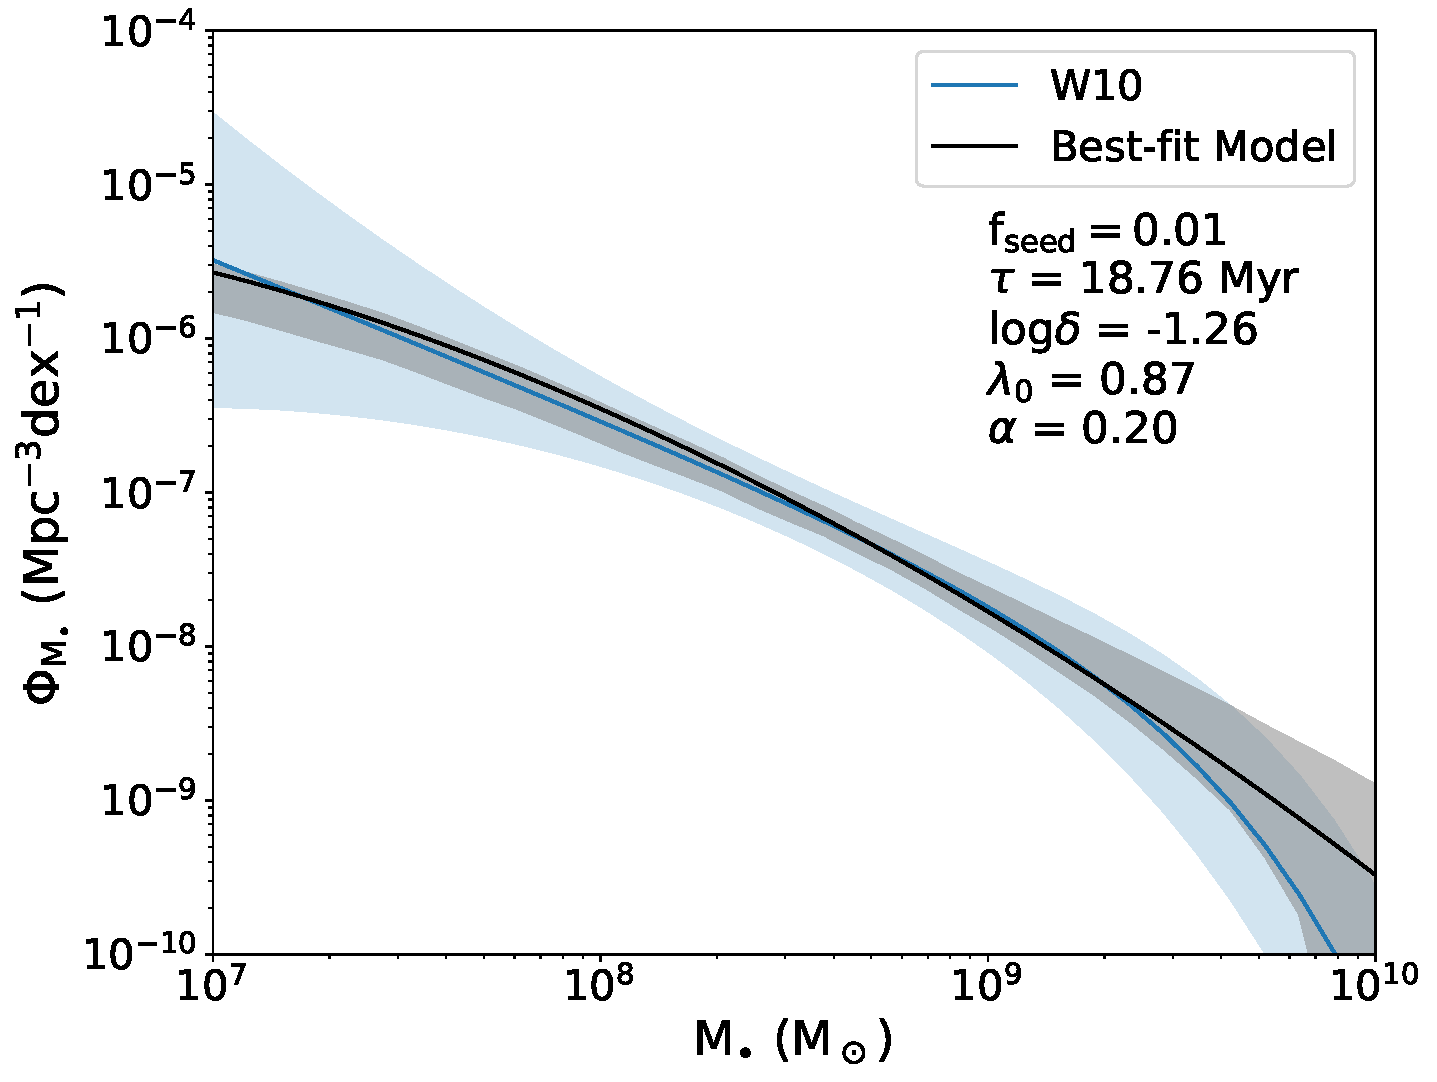
\includegraphics[width=85mm]{f2ndraw60MF_spread.pdf}
\caption{
The BH mass function at $z=6$ with the best-fit parameters (black curve) and the $1\sigma$ spread (shaded region) for the cases with $\fseed=0.1$ (left) and $0.01$ (right). 
For comparison, the BHMF inferred by \citetalias{2010AJ....140..546W} is overlaid (blue curve and shaded region).
The data is used for the model parameter fitting.
%.The blue line shows the BHMF derived by \citet{2010AJ....140..546W}.
% error of observation
}
\label{fig:fitmf}
\end{figure*}


%%%%%%%
%    Fig. 5
%%%%%%%
\begin{figure*}
\centering
%\includegraphics[width=170mm]{fits_LF.png}
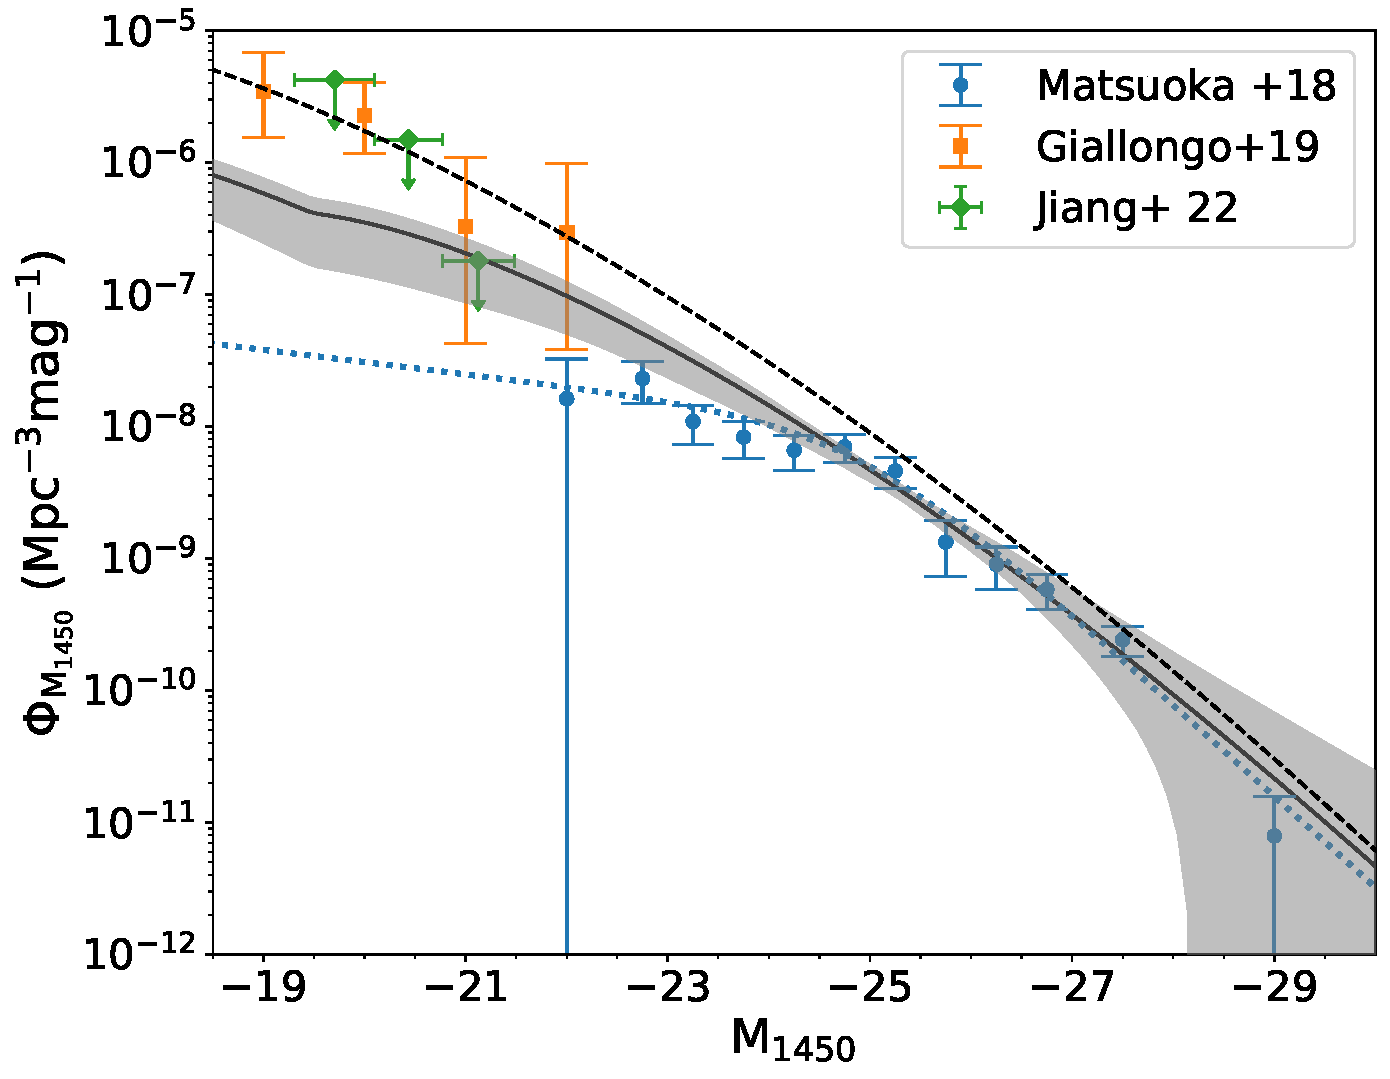
\includegraphics[width=85mm]{f1ndraw60LF_spread.pdf}\hspace{3mm}
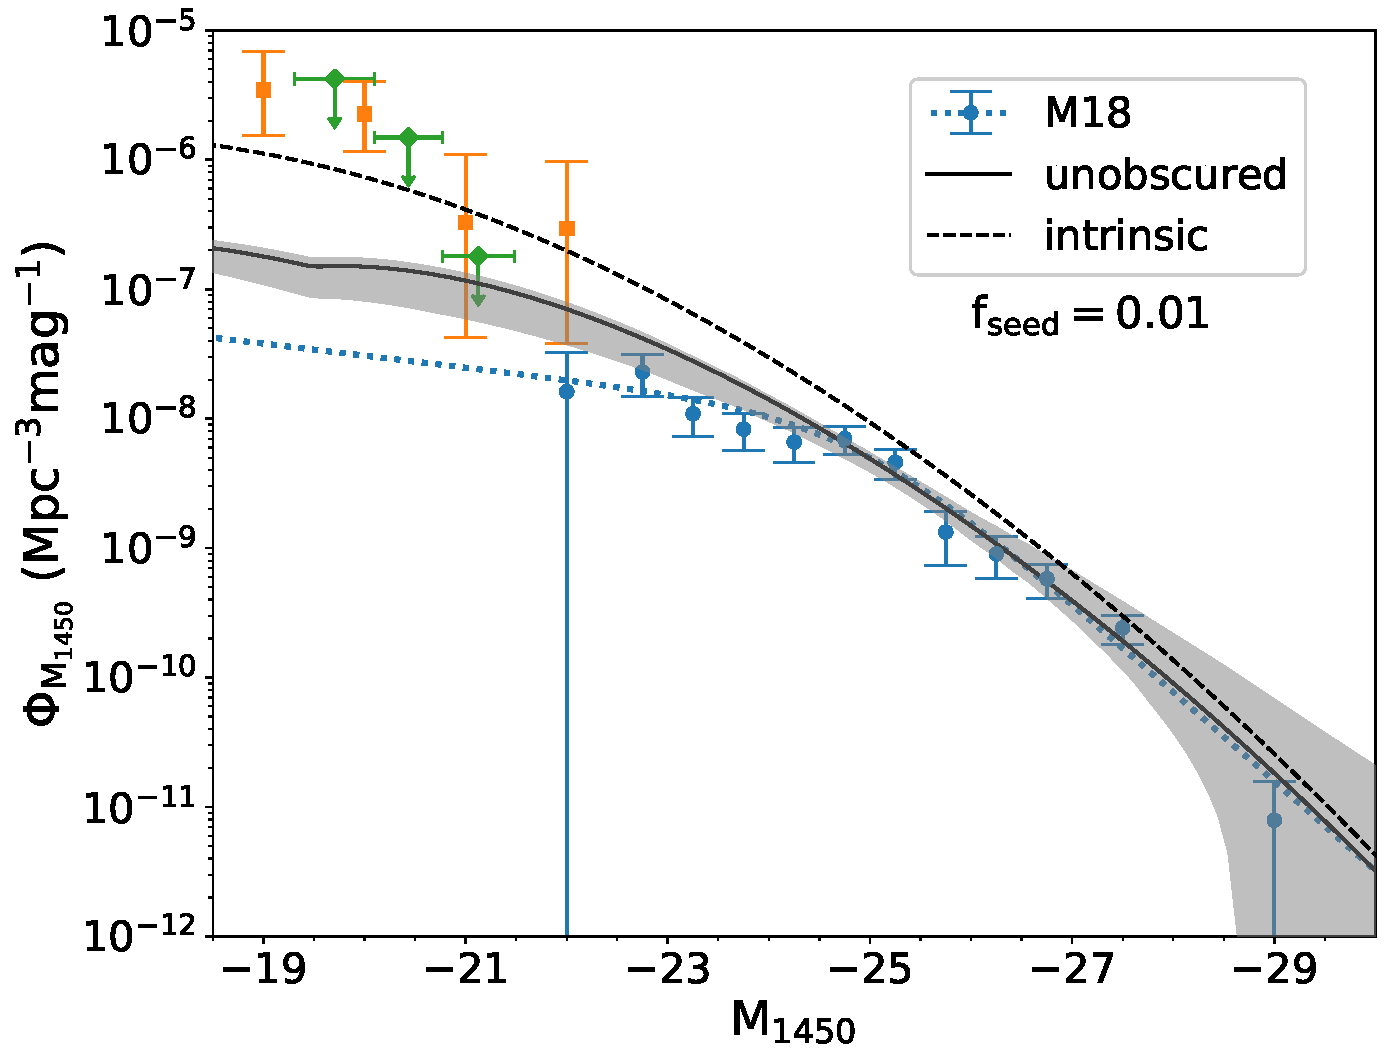
\includegraphics[width=85mm]{f2ndraw60LF_spread.pdf}
\caption{
The unobscured quasar luminosity function at $z=6$ with the best-fit parameters (black solid line) and the $1\sigma$ spread for the cases with $\fseed=0.1$ (left) and $0.01$ (right).
The observed data (blue symbols) with error bars are taken from \citetalias{2018ApJ...869..150M} and is used for the model parameter fitting.
The upper bound of faint quasar number density is derived from the cumulative QLF presented in \citet{2022NatAs...6..850J}.
The X-ray QLF data in the faint end inferred from the $z\sim 5-6.1$ quasar sample in \citet{2019ApJ...884...19G} are denoted by orange symbols,
note that we conduct an extrapolation with quasar number densities scaling with $10^{-0.72\Delta z}$ at $z$ in $5-6$ \citep{2016ApJ...833..222J}.
For comparison, we show the intrinsic QLF predicted by our model in dashed lines.
}
\label{fig:fitlf}
\vspace{2mm}
\end{figure*}



In Fig.~\ref{fig:fitmf}, we show the total BHMF at $z=$ 6 reproduced by the best-fit parameters for 
$\fseed = 0.1$ (left) and $0.01$ (right) as well as the statistical error, 
which is defined as the $1\sigma$ standard deviation calculated from randomly selected parameters from the sampling.
For comparison, we present the BHMF inferred by \citetalias{2010AJ....140..546W} along with the statistical errors.
Note that \citetalias{2010AJ....140..546W} constructed the BHMF using quasar samples with 
$10^8~\Msun \lesssim \Mbh \lesssim 3\times 10^9~\Msun$.
Overall, our best-fit BHMF model agrees with their constraints in this mass range.
The power-law index of the BHMF ($\alpha_{M_\bullet} \equiv \D \ln \Phi_{M_\bullet}/\D \ln M_\bullet$) is as steep as $\alpha_{M_\bullet}\lesssim -1$
at $M_\bullet \gtrsim 10^7~(3\times 10^7)~\Msun$ for $\fseed = 0.1 ~(0.01)$.
The total mass budget of the entire BH population is dominated by BHs with the characteristic mass (see also Section~\ref{sec:cosm}). 
The discrepancy between the model and observational data becomes larger at the high- and low-mass end,
reflecting poor constraints on the BHMF from the current observations.
%The differences at the two extreme ends become smaller with the lower seeding fraction of $\fseed = 0.01$.
%This is because the progenitors of $z=6$ BHs with $10^{7-8}~\Msun$ were the most abundant BH population 
%in the seeding epochs (i.e., a flatter slope of the BHMF; see Fig.~\ref{fig:seedmf}) and mass growth for BHs heavier than 
%$\sim 10^8~\Msun$ is suppressed owing to the high value of $\delta~(\simeq 0.055)$.


%%%%%%%
%    Fig. 6
%%%%%%%
\begin{figure*}
\centering
%\includegraphics[width=175mm]{BHMF_rhoz1.png}
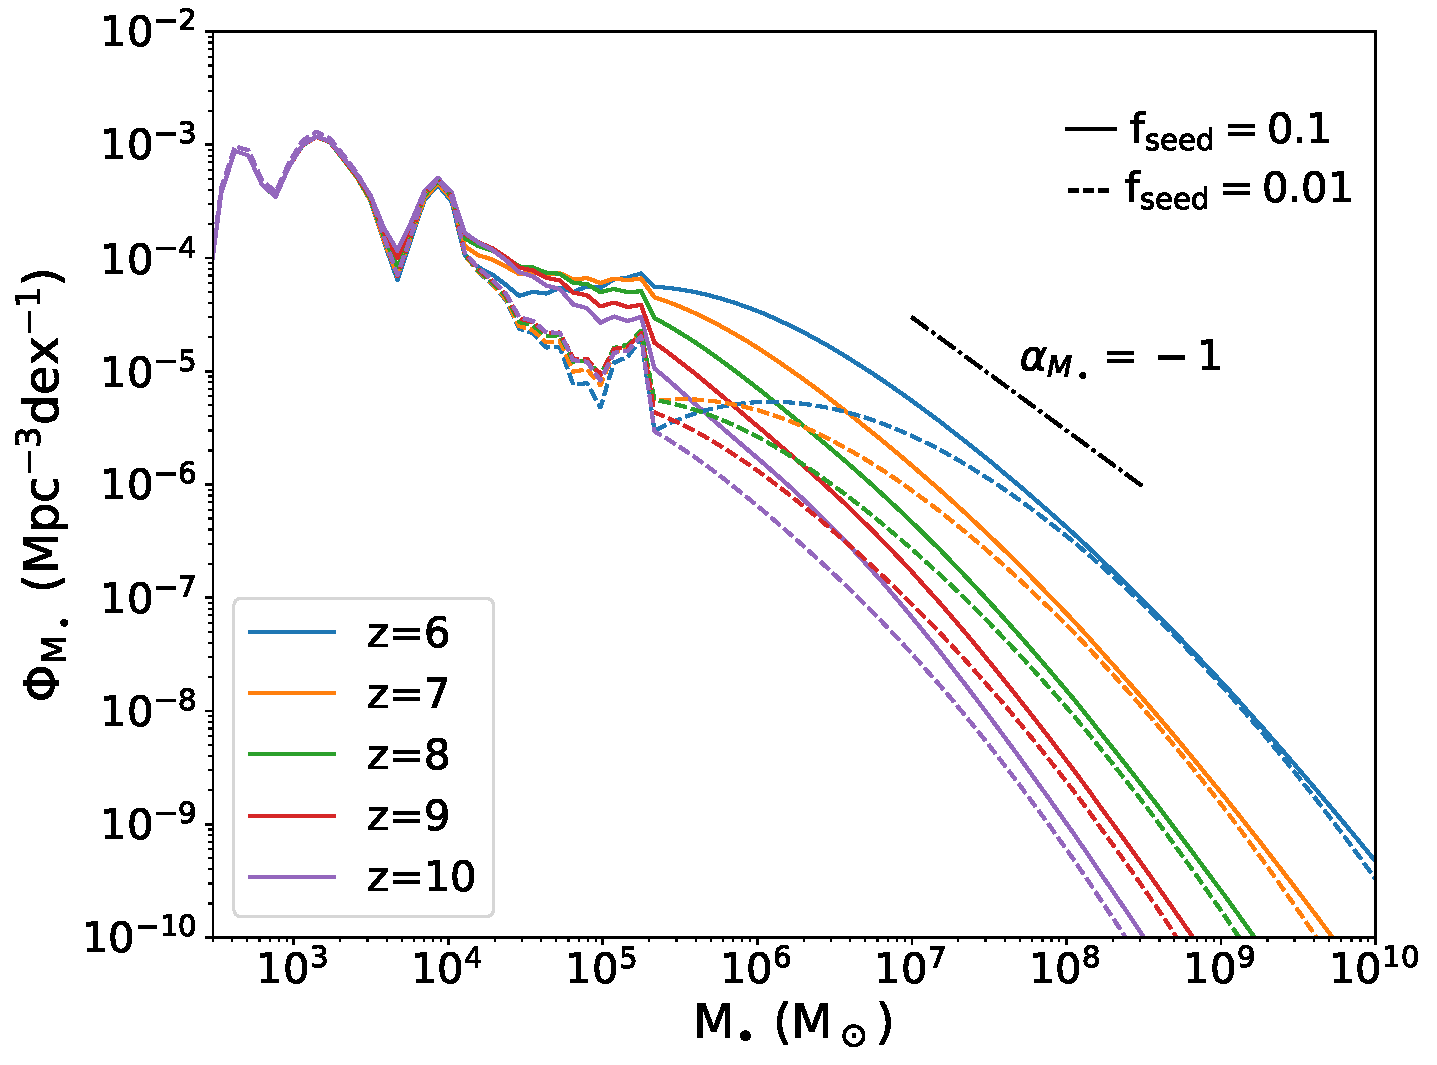
\includegraphics[width=85mm]{MF.pdf}\hspace{5mm}
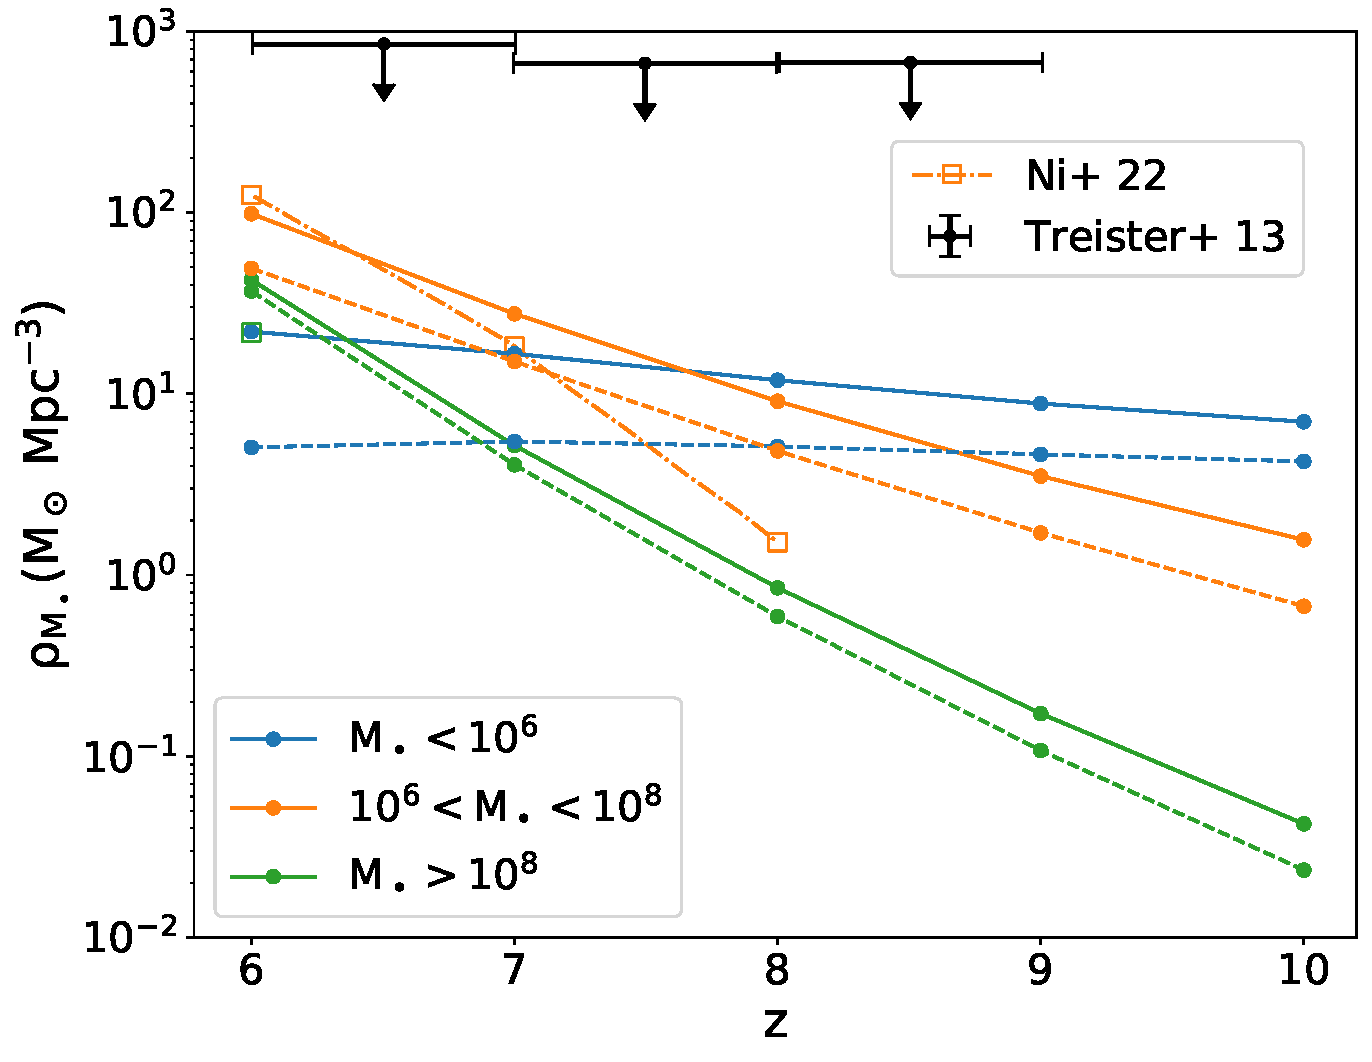
\includegraphics[width=81mm]{rhoM_comb.pdf}
\caption{
{\it Left panel}: BH mass functions predicted by the best-fit models at $z=6-10$,
including a fraction of $\fseed$ seeds evolving by our model assumption and the remaining ($1-\fseed$) fraction with no subsequent growth.
The solid (dashed) lines denote the cases with $\fseed=0.1$ (0.01).
{\it Right panel}: the cumulative mass density evolution for BHs in different mass ranges in a comoving volume, 
evaluated by the integration of the BHMF shown in the left panel.
The dashed-dotted line and open square symbols show the results from \citet{2022MNRAS.513..670N}.
The upper bound of accreted BH mass density from \citet{2013ApJ...778..130T} is denoted by black arrows.
% The evolutionary trend can be approximated as $\rho_\bullet (z) \propto 10^{k_M z}$, where $k_M\simeq -0.68$.
}
\label{fig:BHMF_rhoz}
\vspace{5mm}
\end{figure*}


Fig.~\ref{fig:fitlf} presents the QLFs at $z=6$ reproduced by the best-fit parameters as well as the $1\sigma$ spreads
for $\fseed = 0.1$ (left) and $0.01$ (right).
The solid and dashed curve is the {\it unobscured} and {\it intrinsic} QLF, respectively.
The latter one includes both obscured and unobscured quasars.
For comparison, we overlay the observational data taken from \citetalias{2018ApJ...869..150M} in blue
and their parametric QLF with a double power-law function (dotted curve).
Our best-fit unobscured QLF is consistent with the observed one at $-29~{\rm mag} \lesssim \Muv \lesssim -25~{\rm mag}$,
but overproduces fainter quasars at $\Muv\gtrsim -24~{\rm mag}$.
As seen in the BHMF, the difference between the model and observational data at the faint end becomes smaller with
the lower seeding fraction.
Since the progenitors of those faint quasars were seed BHs located around the peak of the mass distribution,
those BHs naturally produces a flatter slope of the QLF at the faint end.
In addition, we show upper bounds of the faint quasar abundance at $\Muv\gtrsim -22~{\rm mag}$ \citep[green;][]{2022NatAs...6..850J}
based on a search for point sources in the survey fields of the Hubble Space Telescope (HST).
Our unobscured QLF lies within the constraints.


Quasar observations in X-rays also provide 
useful constraints on the intrinsic population because of less obscuration in X-rays.
Based on the X-ray selected faint quasars, \cite{2019ApJ...884...19G} reported a number density of 
faint quasars in orange, which is substantially higher than that expected from extrapolation of the rest-UV based QLF by 
\citetalias{2018ApJ...869..150M} (dotted curve) down to the faint end of $\Muv\gtrsim -22~{\rm mag}$.
In Fig.~\ref{fig:fitlf}, we take their $z=5.55$ luminosity function correcting for redshift evolution 
with a scale factor of $10^{-0.72\Delta z}$ \citep{2016ApJ...833..222J}, where $\Delta z=0.45$.
Our best-fitted intrinsic QLF (dashed curve) is broadly consistent with the faint-end of the X-ray based QLF within the errors.
From another point of view, the discrepancy between the UV and X-ray QLFs at the faint end would be explained by the fact that 
only bright quasars outshining their host galaxies can be identified as point-like sources in the rest-UV quasar selection 
(\citetalias{2018ApJ...869..150M}; \citealt{2020MNRAS.495.2135N,2020MNRAS.494.1771A,2021MNRAS.502.2757O,2021MNRAS.502..662B,2022arXiv220712282K}).
However, at the faint end at $\Muv\gtrsim -24$ mag, extended sources such as the brightest galaxies at $z\sim 6$ 
dominate over quasars in number at the same UV magnitude \citep{2022ApJS..259...20H}.
Thus, the current observations might miss quasars embedded in extended galaxy populations. 
We leave this issue as an important caveat in high-$z$ quasar observations.


\vspace{2mm}
\section{Cosmological evolution of BH mass and quasar luminosity function}\label{sec:cosm}


%%%%%%%
%    Table. 2 
%%%%%%%
\begin{deluxetable*}{lccccccc}%[t!]
\tablecolumns{1}
\renewcommand\thetable{2} %! fix indexing
\tablewidth{0pt} 
\tablecaption{\blue{Detection Number of Quasars Estimated for Future Surveys} \label{tab:N_detect}} %! reference indexing
\tablehead{
  \colhead{Telescope} & \colhead{ Survey area} & \colhead{Photo. depth} &  \colhead{$N(z\sim 6)$} & \colhead{$N(z\sim 7)$}& \colhead{$N(z\sim 8)$}&  \colhead{$N(z\sim 9)$}&  \colhead{$N(z\sim 10)$}\\
  \colhead{} & \colhead{(\rm{deg}$^2$)} & \colhead{(AB mag)} & & & & & 
}
\startdata
Wide RST    &  2000  & $YJH$  27   & $6759_{-3185}^{+15} $ &  $1514_{-558}^{+169}$ &  $349_{-131}^{53}$ & $85_{-48}^{+23}$ & $25^{+12}_{-15}$  \\
Wide RST    &  2000  & $\Muv=-26$ & $21_{-5}^{+13} $      &  $2_{-7}^{+8}$        &  --  & -- & --  \\
Wide Euclid & 15000  & $YJH$  24   & $6654^{+95}_{-2282}$  &  $708^{+213}_{-237}$ &   $93^{+66}_{-56}$ & $14^{+32}_{-27}$ & --  \\
Wide Euclid & 15000  & $YJH$  23   & $2480^{+188}_{-614}$  &  $207^{+144}_{-114}$ &   $23^{+27}_{-19}$ & $3^{+12}_{-10}$ & --  \\
Wide Euclid & 15000  & $\Muv=-26$ & $154^{+100}_{-38}$  &  $12^{+59}_{-50}$ &   $1^{+4}_{-3}$ & -- & --  \\
\enddata
\tablecomments{
Predicted number of quasars at each redshift in the two surveys, with the assumption of the survey volume with $\Delta z =1$ and 100\% completeness.
The integration of QLF starts from the 5$\sigma$ point source detection limits of the $YJH$ bands in each survey, 
and the bright magnitude with $\Muv=-26$ mag.
In addition, detection limit with 22 mag in the $YJH$ bands is examined for Euclid,
mimicking the effect of quasar selection function.% following \citet{2019A&A...631A..85E}.
}
\end{deluxetable*}



Based on the constraint from $z\sim 6$ quasar observations, the best-fit model from the MCMC realizations enables
us to probe the statistical aspect of BH evolution at higher redshifts.
We apply the result to construction of BHMFs and QLFs at $z\geq 6$ and give implications for
the future explorations of high-$z$ quasars.


\subsection{Black Hole Mass Functions}


In the left panel of Fig.~\ref{fig:BHMF_rhoz}, we show the predicted BHMFs at five different redshifts of $z=6-10$
for $\fseed=0.1$ (solid) and $0.01$ (dashed).
As shown in Fig.~\ref{fig:seedmf}, the mass distribution of seed BHs develops up to $M_\bullet \lesssim 2\times10^5~\Msun$ by $z\gtrsim 17$.
Thus, the high-mass tail of the BHMF is produced owing to subsequent growth of seed BHs (i.e., the fraction $\fseed$ of all the seeds).
In fact, the case with $\fseed=0.1$ yields the number density of those growing seeds ten times higher than that with $\fseed =0.01$,
making the difference in the BH abundance at $M_\bullet \sim 10^{5-6}~\Msun$.
%\footnote{For each case, a fraction $(1-\fseed)$ of BHs are assumed to keep the original mass at birth without subsequent growth.}.
This result suggests that the information on the seeding process still remains in the low mass regime.
Toward lower redshifts, heavier BHs with $\gtrsim 10^7~\Msun$ emerge owing to efficient growth
and thus the number density of such massive BHs in the high-mass tail increases.
Since the BHMF shape at $z=6$ is constrained by \citetalias{2010AJ....140..546W},
% BHMF with $M_\bullet \simeq 10^8-3\times 10^9~\Msun$ at $z=6$,
the two cases reproduce similar shape of mass distribution at $M_\bullet \simeq 10^8-3\times 10^9~\Msun$ (see Fig.~\ref{fig:fitmf}).
As a result, the BHMF at $M_\bullet \gtrsim 10^7~\Msun$, which is potentially accessible by quasar observations,
can be characterized with a double power-law function, similar to lower-$z$ quasar populations \citep[e.g.,][]{2013ApJ...764...45K,2015MNRAS.447.2085S}.
%while the difference in the two BHMF shapes is profound toward the low mass range of $M_\bullet \lesssim 10^7~\Msun$.
%The BH abundance and shape of the mass distribution at $10^5 \lesssim M_\bullet/\Msun \lesssim 10^7$ depend on the seeding fraction,
%while the distributions converge at $M_\bullet \gg 10^7~\Msun$ toward $z= 6$. 
%This result suggests that the information on the seeding process would still remain in the low mass regime of $M_\bullet \lesssim 10^7~\Msun$.
%
%The different seeding fraction varies the characteristic BH mass where the BHMF slope is close to $\alpha_{M_\bullet}\simeq -1$,
%i.e., the typical masses which dominate the cumulative mass density (see Section~\ref{sec:fitting_result}). 
% the difference is also shown by the mass ranges where the slope of BHMF is close to $\alpha_{M_\bullet}\simeq -1$,
%i.e., the typical masses which dominate the cumulative mass density (see Section~\ref{sec:fitting_result}). 
%In the case of $\fseed=0.01$, this typical mass range is higher, despite the integrated mass density is lower than that with $\fseed=0.1$.




In the right panel of Fig.~\ref{fig:BHMF_rhoz}, we present the cumulative mass density of BHs in a comoving volume
for $\fseed=0.1$ (solid) and $0.01$ (dashed),
defined by the integration of the BHMF as
%
\begin{equation}
 \rho_\bullet(z)=\int_{\mathcal{I}} \Phi_{\Mbh} (z) \Mbh ~\D \log \Mbh.
\end{equation}
%
Here, we consider three mass ranges: $M_\bullet \leq 10^6~\Msun$ (blue), $10^6~\Msun < M_\bullet < 10^8~\Msun$ (orange),
and $M_\bullet \geq 10^8~\Msun$ (green).
Overall, the mass density of the heaviest BHs quickly grows toward lower redshifts,
while the mass density barely evolves for the lightest BHs.
At $z\lesssim 7-8$, more massive BHs with $\gg 10^6~\Msun$ begin to dominate the total mass budget of the entire BH population,
promoting the so-called downsizing or anti-hierarchical evolution of massive BHs 
in terms of mass occupation \citep[e.g.,][]{2014ApJ...786..104U}.
Note that the characteristic mass in the BHMF (i.e., $\alpha_{M_\bullet}=-1$) is $M_\bullet \simeq 10^7~(3\times 10^7)~\Msun$ for 
$\fseed=0.1~(0.01)$.
Moreover, as shown in the left panel, the mass-density evolution is affected by the choice of the seeding fraction more substantially
for less massive BHs that keep the information on their initial conditions at birth.



For comparison, we overlay the BH mass density evolution with $10^6<M_{\bullet}/\Msun<10^8$
%, and $M_\bullet>10^8~\Msun$
obtained from the cosmological simulations in \citet{2022MNRAS.513..670N} (dashed-dotted curve).
At $z\lesssim 7$, our results are in overall good agreement with those simulation results.
However, our models predict a larger number of $10^{6-8}~\Msun$ BHs emerging at $z\sim 10-8$,
owing to our model prescription that allows BH seed formation earlier on and (modest) super-Eddington episodes.
Furthermore, the measured unresolved fraction of the cosmic X-ray background constrains
the global accretion history of massive BHs at $z>5$ \citep{2012A&A...545L...6S,2013ApJ...778..130T}.
Upper bounds on the accreted-mass density onto massive BHs (black arrows) prohibits overproduction of low mass BHs at cosmic dawn.
Our quasar sample in the biased, overdense region of the universe (haboring DM halos with $\Mh\gtrsim 10^{11}~\Msun$) 
are consistent with the constraint, unlike models that require a large number of stellar-mass BH remnants.





\if0
Varying the minimum mass as $M_{\rm min}=10^7$, $10^8$, and $10^9~\Msun$,
we find that the early BH assembly takes place rapidly and the redshift-dependence can be approximated by
%
\begin{equation}
\rho_\bullet(z)
%= \rho_{\bullet 0}\cdot e^{k_{\rm M}(z-6)}
\simeq \rho_{\bullet,0}~ 10^{k_{\rm M}(z-6)},
\end{equation}
%
where the fitted values of $\rho_{\bullet,0}$ and $k_{\rm M}$ are shown in Table.~\ref{tab:MFz}.

On the other hand, the stellar mass density of the quasar progenitor halos is calculated as
%
\begin{equation}
\rho_{\star}(z)
\simeq f_\star n_{\Mh} M_h~ 10^{k_{\rm h}(z-6)},
\end{equation}
%
where $f_\star(\equiv M_\star/\Mh)$ is the mass ratio of the galaxy stellar mass to the DM halo mass and
$n_{\Mh}$ is the number density of quasar host halos with $\Mh$ in a comoving volume at $z=6$; namely,
the value of $n_{\Mh}\Mh \simeq (6.2-99)\times 10^6~\Msun~{\rm Mpc}^{-3}$.
We here express the mass growth of the DM halo with a functional form of $\propto 10^{k_{\rm h} z}$,
which can describe the mass growth of DM halos
\citep[e.g.,][]{2002ApJ...568...52W,2008MNRAS.383..615N,2008MNRAS.388.1792N,2010MNRAS.406.2267F}
\footnote[4]{
In fact, this redshift dependence leads to a halo-mass growth rate of $\D \left(\ln \Mh \right) / \D t \propto(1+z)^{5/2}$,
which has been understood based on the extended Press-Schechter formalism and also derived by
a fit to merger trees from cosmological N-body simulations \citep{2013MNRAS.435..999D}.}.
% The redshift dependence yields the cosmic BH growth rate in the matter-dominated universe
% as $\dot{\rho}_\bullet \propto \rho_\bullet (1+z)^{5/2}$ or

% \begin{align}
% \dot{\rho}_\bullet(z) & =\dot{\rho}_\bullet(z=6)\left(\frac{1+z}{7}\right)^{5/2} 10^{k_{\rm M}(z-6)}, \\
% &\simeq *** ~\Msunyr~{\rm Mpc}^{-3} \left(\frac{1+z}{7}\right)^{5/2} e^{\bar{k}_{\rm M}(z-6)},\nonumber
% \end{align}

% where $\bar{k}_{\rm M} \equiv k_{\rm M} \ln 10 \simeq -1.84$.
% \red{KI: I'm not sure what we discuss here... One thing is the cosmic SFR density (Madau's plot).
% Is there something like Madau's plot but for DM halos?}
% The exponential dependence on redshift is reminiscent of the cosmic galaxy mass growth
% $M_{\star} \propto e^{-B z}$, as a consequnce of the assumption of fixed galaxy to DM halo mass ratio,
% and the growth rate of DM halos in the extended Press-Schechter formalism
% $\D \left(\ln \Mh \right) / \D t \propto(1+z)^{5/2}$ \citep{2008MNRAS.383..615N}.
% Our results suggest that the cumulative massive BH mass density growing in galactic nuclei also follows
% an exponential evolution with redshift,
% which is statistically in agreement with the host halo and galaxy growth.
The star-to-halo mass ratio is assumed to be $f_\star =0.01$ for those quasar progenitor halos at $z>6$
% (UNIVERSEMACHINE; Behroozi et al. 2019).
\citep[fits by code {\tt UNIVERSEMACHINE} in][]{2019MNRAS.488.3143B}.
%https://ui.adsabs.harvard.edu/abs/2019MNRAS.488.3143B/abstract
With those values, we estimate the stellar-to-BH mass ratio for high-$z$ quasars as
%
\begin{equation}
\frac{\rho_{\star}(z)}{\rho_{\bullet}(z)}
\simeq 2.5\times 10^{3} \left(\frac{f_\star}{0.01}\right)
~ 10^{(k_{\rm h}-k_{\rm M})(z-6)},
\end{equation}
% 
where $k_{\rm h} \approx -0.16 $ for the parent halo growth histories.
Therefore, at $z\sim 6$ the bulge-to-BH mass ratio $\sim O(10^3)$ for the entire BH population (i.e., low-mass BHs and low-luminosity quasars) 
\blue{
is broadly consistent with those seen in the local universe \citep[$\simeq 200-1000$ in e.g.,][]{2012ApJ...751L..25V,2013ARA&A..51..511K},
although SMBHs observed as high-$z$ quasars appear to be $\sim 10$ times overmassive compared to the local relation 
\citep[e.g.,][]{2013ApJ...773...44W,2020A&A...637A..84P,2021ApJ...911..141N}.
Our result suggests that overall the build-up of stellar mass in galaxies is earlier than BHs,
which will be tested by high-$z$ galaxy and quasar surveys.
}

%%%%%%%
%    Table. 1 
%%%%%%%
\begin{table}
\renewcommand\thetable{1} %! fix indexing
\caption{$\rho_\bullet(z)$ Evolution Parameters}
\begin{center}
% \tablenum{1}
\begin{tabular}{l c r}
\hline
\hline
$M_{\rm min}$ & $\log \rho_{\bullet,0}$ & $k_{\rm M}$ ~~~ \\ 
\hline 
10$^7$  &  $ 1.81\pm 0.28$  &  $-0.68 \pm 0.21$  \\
10$^8$  &  $ 1.54\pm 0.47$  &  $-0.84 \pm 0.31$  \\
% 10$^9$  &  $-8.30_{-0.47}^{+0.47}$  & $-1.04_{-0.58}^{+0.54}$ \\
10$^9$  &  $ 1.01\pm 0.47$  &  $-1.01 \pm 0.58$ \\
\hline 
\end{tabular}
\label{tab:MFz}
\end{center}
\end{table}    
\fi


\subsection{Quasar Luminosity Functions}
\label{sec:qlfglf}


%%%%%%%
%    Fig. 7
%%%%%%%
\begin{figure*}[h!]
\centering
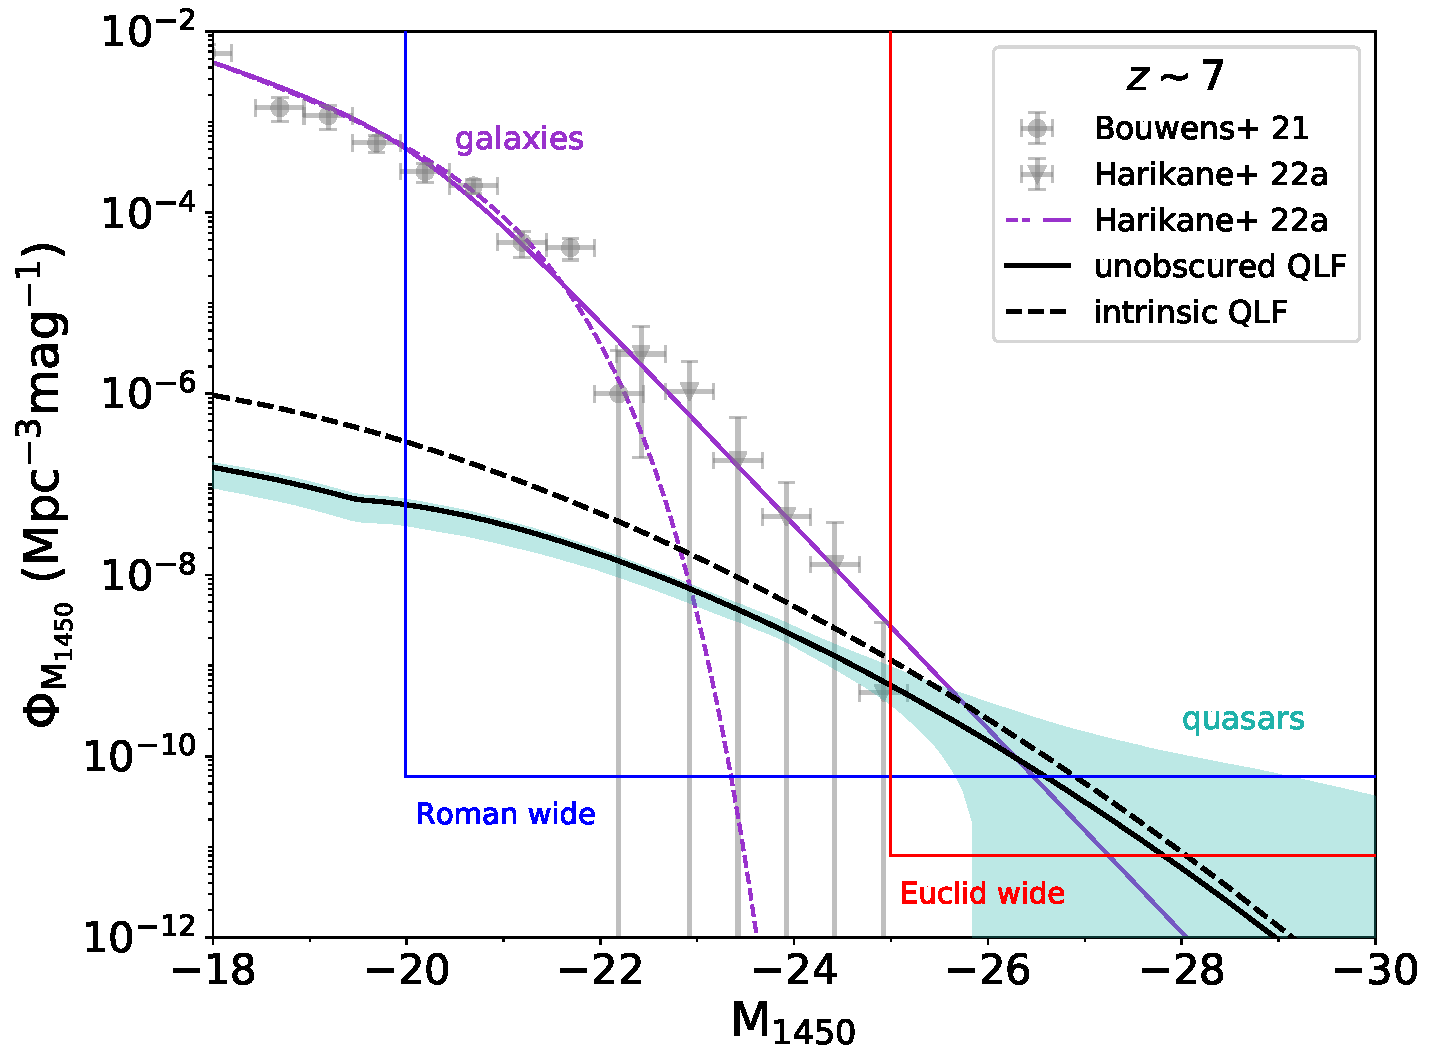
\includegraphics[width=85mm]{LF_spreadz7.pdf}\hspace{2mm}
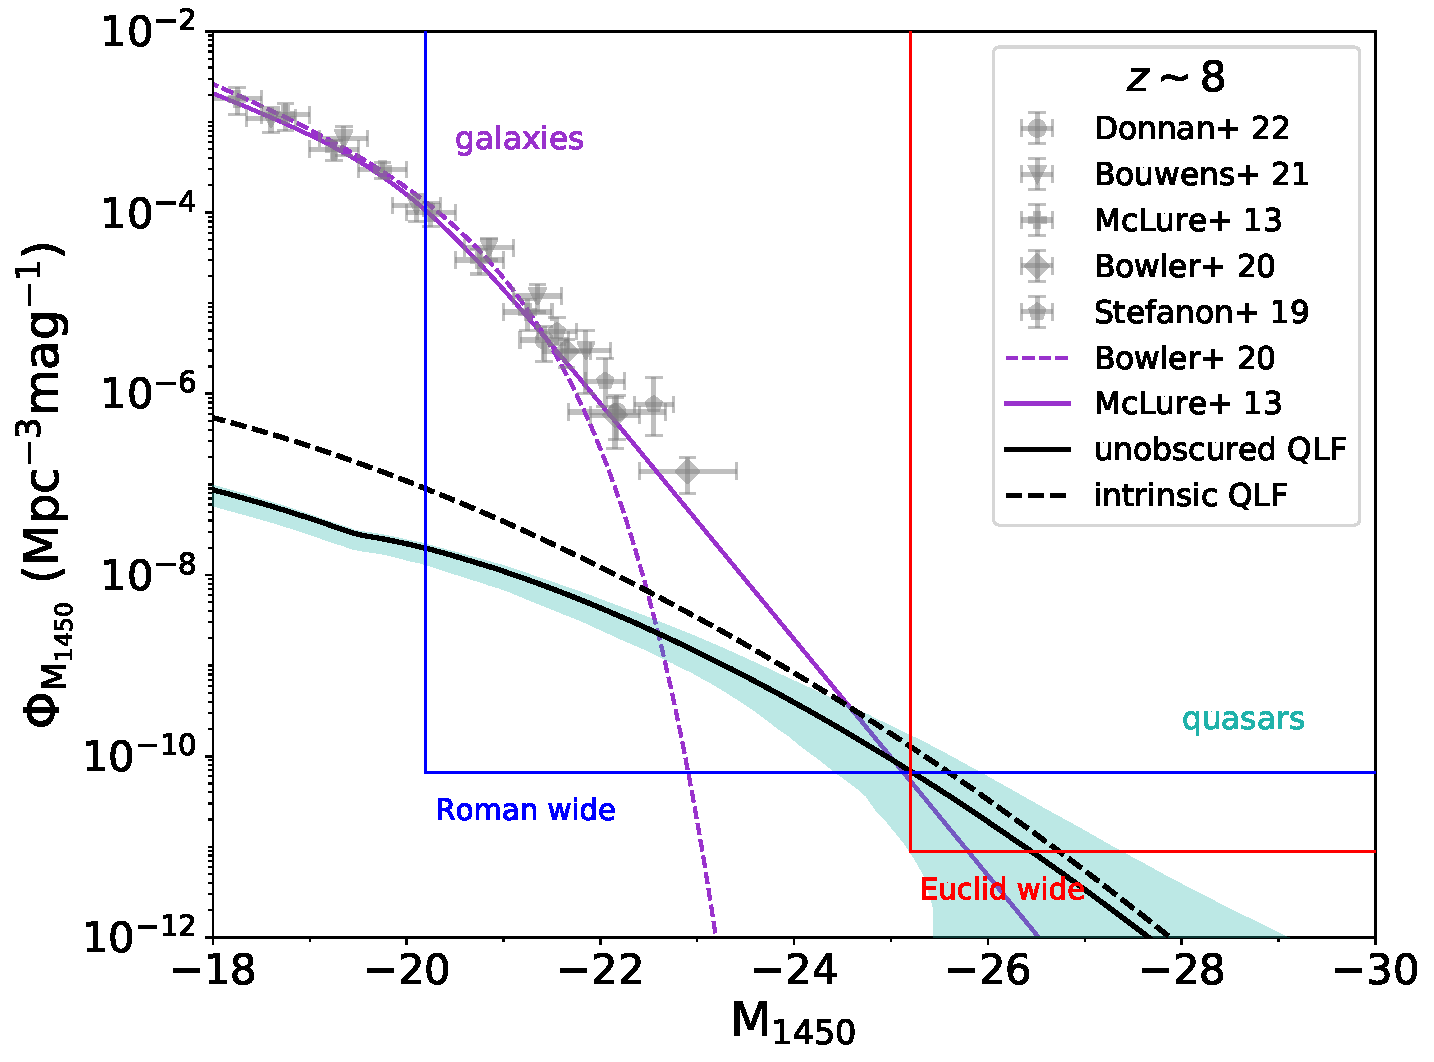
\includegraphics[width=85mm]{LF_spreadz8.pdf}\\\vspace{5mm}
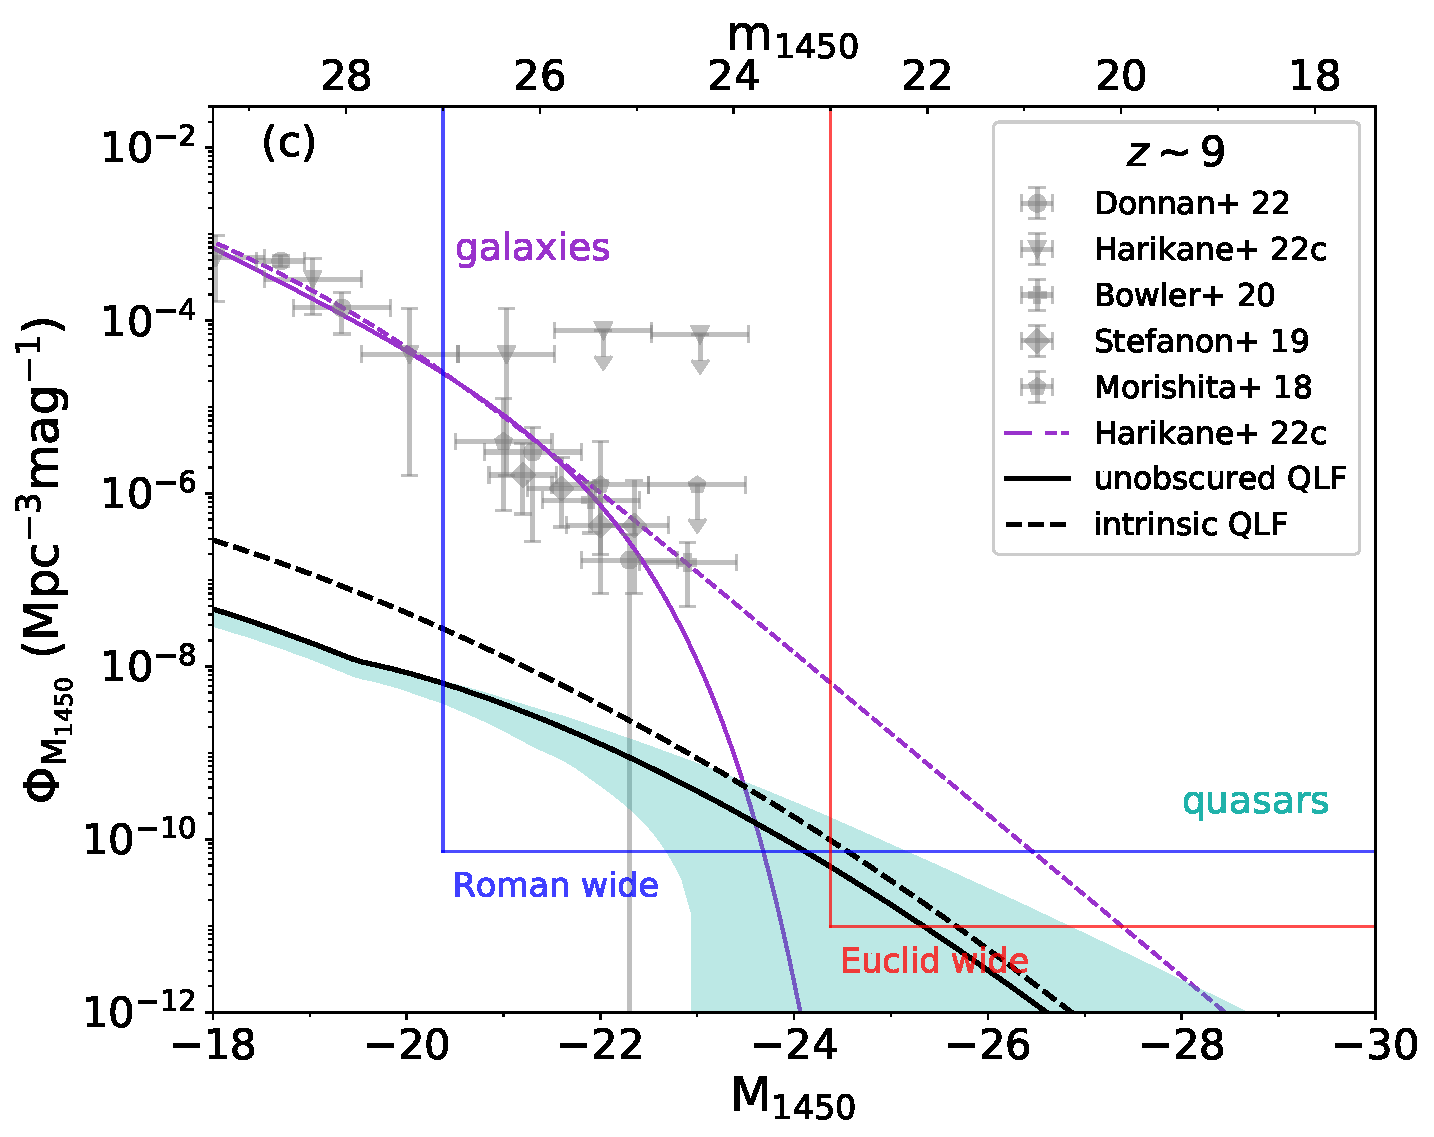
\includegraphics[width=85mm]{LF_spreadz9.pdf}\hspace{2mm}
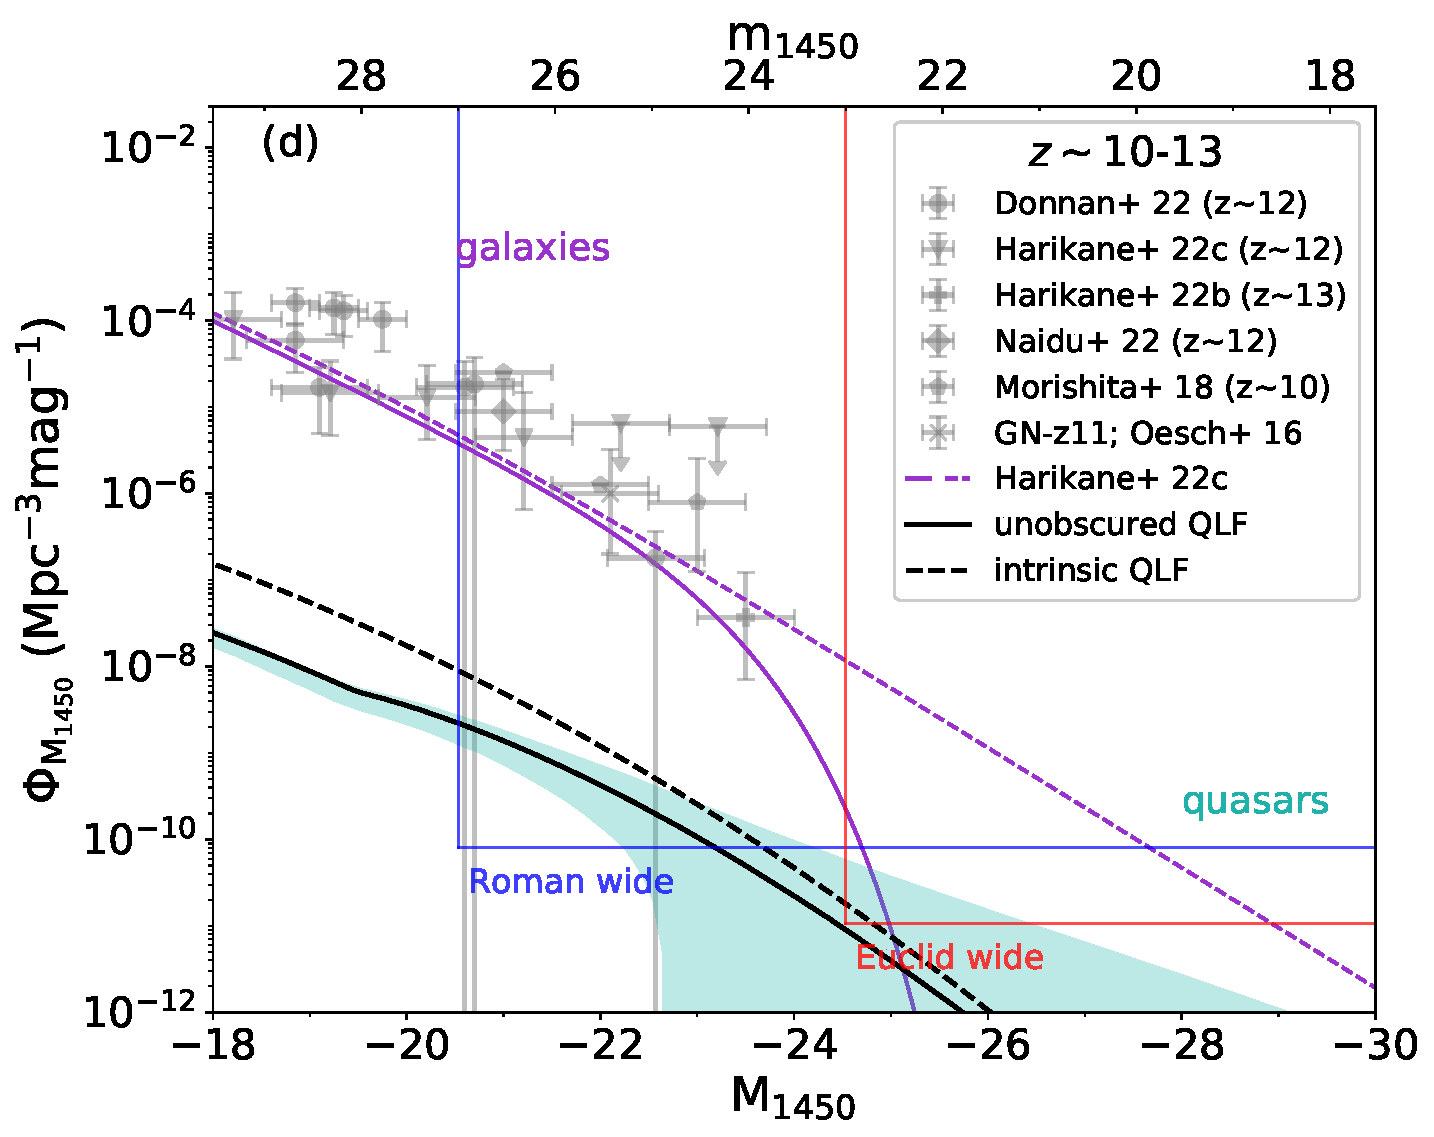
\includegraphics[width=85mm]{LF_spreadz10.pdf}
\caption{Predicted quasar luminosity functions and depths and volumes of upcoming surveys.
The black solid and dashed curves present the QLF for the unobscured population (e.g., type-I AGNs) 
and the whole population (i.e., type-I and type-II AGNs), and the shaded region presents the $1\sigma$ spread.
The expected depths and volumes of future surveys with Wide RST and Wide Euclid are overlaid with the blue lines,
indicating the detectability of quasars at these redshifts.
Galaxy UV luminosity functions are plotted with the data points (grey) and fitting functions with a Schechter (dotted curve) and double power-law (dash-dotted curve) shape.
The galaxy luminosity function data at $z\sim$ 7 are taken from \citet{2022ApJS..259...20H} and \citet{2021AJ....162...47B}. 
At $z\sim$ 8, the data points are from \citet{2021AJ....162...47B},
\citet{2022arXiv220712356D}, \citet{2013MNRAS.432.2696M}, \citet{2020MNRAS.493.2059B}, and \citet{2019ApJ...883...99S}.
At  $z\sim$ 9, those data are from \citet{Harikane_2022c}, \citet{2022arXiv220712356D}, \citet{2020MNRAS.493.2059B}, \citet{2019ApJ...883...99S}, 
and \citet{2018ApJ...867..150M}.
At $z\sim$ $10-13$, we take data from \citet{Harikane_2022c}, \citet{2022arXiv220712356D}, \citet{Harikane_2022b}, \citet{2022arXiv220709434N}, \citet{2018ApJ...867..150M}, 
and \citet{2016ApJ...819..129O}.
The fitting forms of the luminosity functions are given by \citet{2022ApJS..259...20H} at $z\simeq 7$, 
\citet{2020MNRAS.493.2059B} and \citet{2013MNRAS.432.2696M} at $z\simeq 8$, and \citet{Harikane_2022c} at $9\lesssim z\lesssim 13$.
}
\label{fig:LFs}
\end{figure*}


\if0
Next, we show our prediction of $z=6-10$ unobscured QLFs taken from the BH growth model in the left panel of Fig.~\ref{fig:QLFmag_z}.
Similar to the BHMF, for all the redshift range, the shape of the QLF is well approximated with a double power-law function.
From higher to lower redshifts, the number density of luminous quasars increases and the bright-end of the distribution rises.
% %The model QLFs we propose give interesting prediction and will be further constrained by higher redshift quasar observations.
% \red{KI: add more explanations about the QLFs. How about the detection limits of Euclid, Roman, and others?
% Also, you could compare your results with Aaron Yung's results.}
In the right panle of Fig.~\ref{fig:QLFmag_z}, we present the number density of luminous quasars with $\Muv <-26~{\rm mag}$ as a function of redshift.
The evolutionary trend can be fitted as $\propto 10^{k_{\rm L}z}$, where $k_{\rm L}\approx -0.97$.
Observationally, a rapid decay of the quasar number density toward higher redshifts is found by previous studies
\citep[e.g.,][]{2001AJ....122.2833F,2013ApJ...768..105M,2016ApJ...833..222J,2019ApJ...884...30W},
which show $k_{\rm L}= -0.47$ and $-0.72$ from the analysis of quasar samples at $z\simeq 3-5$ and $z\simeq 5-6$, respectively.
% Recently, a steeper decline of luminous quasar number density toward higher redshifts is proposed by \citet{2019ApJ...884...30W},
% suggesting $k_{\rm L}=-0.78$ at $6\lesssim z \lesssim 7$.
The rapid decline toward higher redshifts is characterized by the treatment of episodic natures of BH accretion with a finite value of
$\tau ~(\simeq 20~{\rm Myr})$, in order to match the statistical properties of high-$z$ quasars.
We also note that the tendency would be explained by the rarity of massive quasar-host halos at higher redshifts,
non-constant radiative efficiencies that covert the BH growth rate into the luminosity, or some combination of these effects
\citep[e.g.,][]{2010ApJ...718..231S}.
%Studies with the assumption of the close correlation of DM halo mass with central BH mass, and a constant Eddington ratio 
%interprete this rapid decline by the rarity of massive halos toward higher redshifts \citep[e.g.,][]{2010ApJ...718..231S}, 
%while another entangling factor is the radiative efficiency in converting BH growth rate to luminosity. 
%In our work, we argue that the episodical BH accretion with bursts and quiescent phases is 
%important in matching the $z\sim 6$ quasar observations, 
%and this calls consideration of the more realistic BH-galaxy coevolution in understanding the observable AGN properties.
\fi

Fig.~\ref{fig:LFs} presents our prediction of QLFs at $z>6$ taken from the BH growth model.
We divide the cosmological QLF evolution into four different epochs; (a) $z\simeq 7$, (b) $z\simeq 8$, (c) $z\simeq 9$, and (d) $z\simeq 10-13$.
The black solid and dashed curve presents the QLF for the unobscured population 
and entire population (including unobscured and obscured quasars), respectively.
The obscured fraction based on X-ray samples \citep{2014ApJ...786..104U} is applied to faint objects, 
but the correction factor is highly uncertain at the faint end of $\Muv\gtrsim -20$ mag.
Similar to the BHMF, for all the redshift range, the shape of the QLF is well approximated with a double power-law function.
From higher to lower redshifts, the number density of luminous quasars increases and the bright-end of the distribution rises.

\blue{
We overlay the expected depths and survey volumes of upcoming near-infrared surveys by
Euclid \citep{2011arXiv1110.3193L} and RST \citep{2019arXiv190205569A}.
Here we consider only their wide-area survey layers because other survey programs are not suitable for quasars at $z\gtrsim 7$.
Table~\ref{tab:N_detect} summarizes the coverage and limiting magnitudes in each survey
and lists the expected detection number of quasars.
In priniciple, Euclid will identify quasars up to $z\sim 8$ and discover $O(100-1000)$ quasars at $z\simeq 7-8$.
The RST will potentially be able to explore the very faint ($\Muv>-22$ mag) but abundant quasar population even at $z\gtrsim 10$. 
%in principle, after subtracting galaxy contaminants.
Note that we do not take into account selection criteria to differentiate quasars from other astrophysical sources such
as Galactic brown dwarfs, strong Balmer-break galaxies, and extremely dusty star-forming galaxies at intermediate redshifts.
Therefore, our estimate in Table~\ref{tab:N_detect} gives an upper bound of the number of detectable high-$z$ quasars.
Nevertheless, this simplified assumption yields $\approx 3-7$ times higher values than those predicted by \citet{2019A&A...631A..85E}.
%Studies that take into account contamination from MLT dwarfs and compact early-type galaxies and quasar selction method
%have confirmed the capability of these surveys in searching high-$z$ quasars \citep{2019A&A...631A..85E,2019BAAS...51c.121F}.
%With the simplified assumption of $100\%$ selection function against contaminants,
%our predicted yield of high-$z$ quasars for the Euclid wide survey is a few times higher than that by \citet{2019A&A...631A..85E}.
%Therefore, our estimation should represent an upper bound of the potentially detectable quasar population.
}
% me:On the other hand, we the selection effect to miss some quasars, especially the faint ones. Our prediction is 



We also show the galaxy UV luminosity function in each panel
along with the fitting functions in a Schechter (dotted) and double power law (dashed-dotted) shape extended to the brighter end
\citep{2013MNRAS.432.2696M, 2016ApJ...819..129O, 2018ApJ...867..150M, 2019ApJ...883...99S, 2020MNRAS.493.2059B,
2021AJ....162...47B, 2022arXiv220712356D,
2022ApJS..259...20H, Harikane_2022b, Harikane_2022c, 2022arXiv220709434N}.
Galaxies at $\Muv\gtrsim -23$ mag dominate quasars in number at all the redshifts and make it 
difficult to identify rare quasars among those faint objects.
Since extrapolated galaxy LFs with a Schechter shape decline quickly with the luminosity increasing,
the abundance of galaxies and quasars becomes comparable around $\Muv \sim -23$ mag ($z=7-8$), $-24$ mag ($z=9$), and $-25$ mag ($z=10-13$).
On the other hand, if the bright end of the galaxy LFs are extended with a power law, those critical UV magnitudes shift to 
$\Muv\sim-26$, $-25$, and $\ll -30$ mag for each redshift range.
Future deep and wide surveys will unveil the relative contribution of the two populations and impacts on cosmic reionization.



%%%%%%%
%    Fig. 8
%%%%%%%
\begin{figure}
\centering
%\includegraphics[width=160mm]{QLF_rhoz.png}
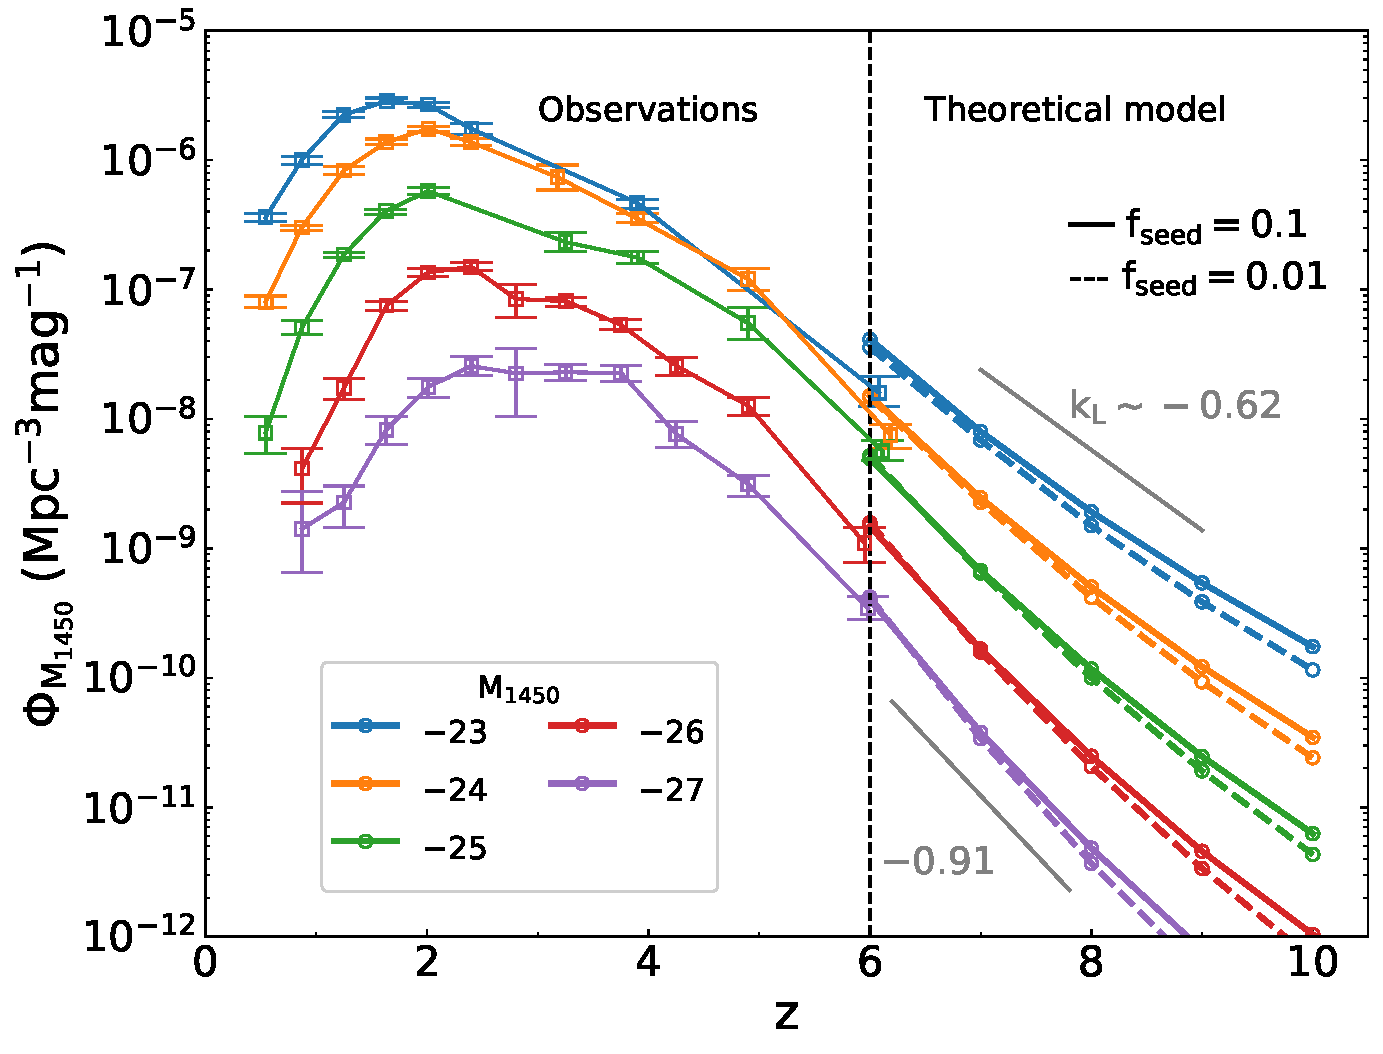
\includegraphics[width=80mm]{QLFmag_z.pdf}
\caption{
Evolution of quasar luminosity functions at different UV magnitudes.
The theoretical prediction from $z=6$ to $10$ for the cases of $\fseed=0.1$ and 0.01 are denoted by solid and dashed lines, respectively.
From theoretical models, the slope is estimated as $k_\mathrm{L} \simeq -0.91$ and $-0.62$ for quasars at $\Muv=-27$ and $-23$ mag, respectively.
The observational data at lower redshifts $z\sim 0-6$ are from the Subaru HSC results \citep{2018PASJ...70S..34A,2018ApJ...869..150M,2020ApJ...904...89N},
SDSS \citep{2006AJ....131.2766R,2013ApJ...768..105M},
the 2dFSDSS LRG and Quasar Survey (2SLAQ; \citealt{2009MNRAS.399.1755C}),
and the Spitzer Wide-area Infrared Extragalactic Legacy Survey (SWIRE; \citealt{2008ApJ...675...49S}).
}
\label{fig:QLFmag_z}
\vspace{5mm}
\end{figure}


In Fig.~\ref{fig:QLFmag_z}, we present the quasar number density as a function of redshift for 
$\fseed =0.1$ (solid) and $0.01$ (dashed).
Each curve corresponds to the value at a UV magnitude from $\Muv=-27$ mag to $-23$ mag.
Our theoretical predictions are shown at $z\geq 6$ (thick curves),
while observational results summarized in \cite{2020ApJ...904...89N} are compiled at lower redshifts (thin curves).
The evolutionary trend can be fitted as $\propto 10^{k_{\rm L}z}$,
where $k_{\rm L}\simeq -0.91$ and $-0.62$ for the brightest and faintest population
at $z\gtrsim 6$, respectively.
A rapid decay of the luminous quasar abundance at $\Muv<-26$ mag toward higher redshifts is found by 
previous observational studies \citep[e.g.,][]{2001AJ....122.2833F,2013ApJ...768..105M,2016ApJ...833..222J,2019ApJ...884...30W}.
For instance, \citet{2019ApJ...884...30W} proposed a decay index of $k_{\rm L}=-0.78\pm{0.18}$ at $6\lesssim z \lesssim 7$,
consistent with our model prediction where $k_\mathrm{L} \simeq -0.84$.


\vspace{2mm}
\section{Discussion}\label{sec:discussion}
\vspace{2mm}
\subsection{Individual BH growth}\label{sec:evol}

From the BH growth model described in Section~\ref{sec:MF}, we further explore individual BH evolutionary tracks starting from the BH seeding phases.
We generate a sample of 10$^6$ BHs, whose formation time and mass distribution at birth follow the model described in Section~\ref{sec:seed}. 
Adopting the best fit parameters in the case of $\fseed = 0.01$, in every time interval $\tlife=18.76$ Myr,
we assign a constant Eddington ratio generated from the Schechter-type ERDF characterized by $\lambda_0=0.87$ and $\alpha=0.20$ 
(see Section~\ref{sec:fitting_result}).
With these parameters, we grow the individual BHs until $z=6$ and study their statistical properties in producing massive BHs.


First, we estimate the duty cycle between at $6\leq z\leq 10$ defined as $f_{\rm duty} \equiv \mathcal{N}\tlife/\Delta t_{\rm H}$, 
where $\mathcal{N}$ is the frequency of super-Eddington accretion bursts with $\lambda \geq 1$ and $\Delta t_{\rm H}\simeq 450$ Myr.
For BH populations grown to $M_\bullet>10^7$, $10^8$ and $10^9~\Msun$ at $z=$ 6,
the average duty cycle is found to be $\langle f_{\rm duty}\rangle \simeq 0.12$, 0.15, and 0.19
(i.e., $\Delta t_{\rm H} \times f_{\rm duty} \simeq 55$, 69, and 85 Myr), respectively.
On the other hand, the average duty cycle for the entire BH population is calculated as $f_{\rm duty}= 0.075$,
adopting this ERDF (see Section~\ref{sec:fitting_result}), which is significantly lower than those for massive BH sub-samples.
Therefore, we suggest that SMBHs observed in $z\simeq 6$ quasars are biased in a way that
the more massive populations undergo longer active accretion episodes along their growth.


%%%%%%%
%    Fig. 9
%%%%%%%
\begin{figure*}
\centering
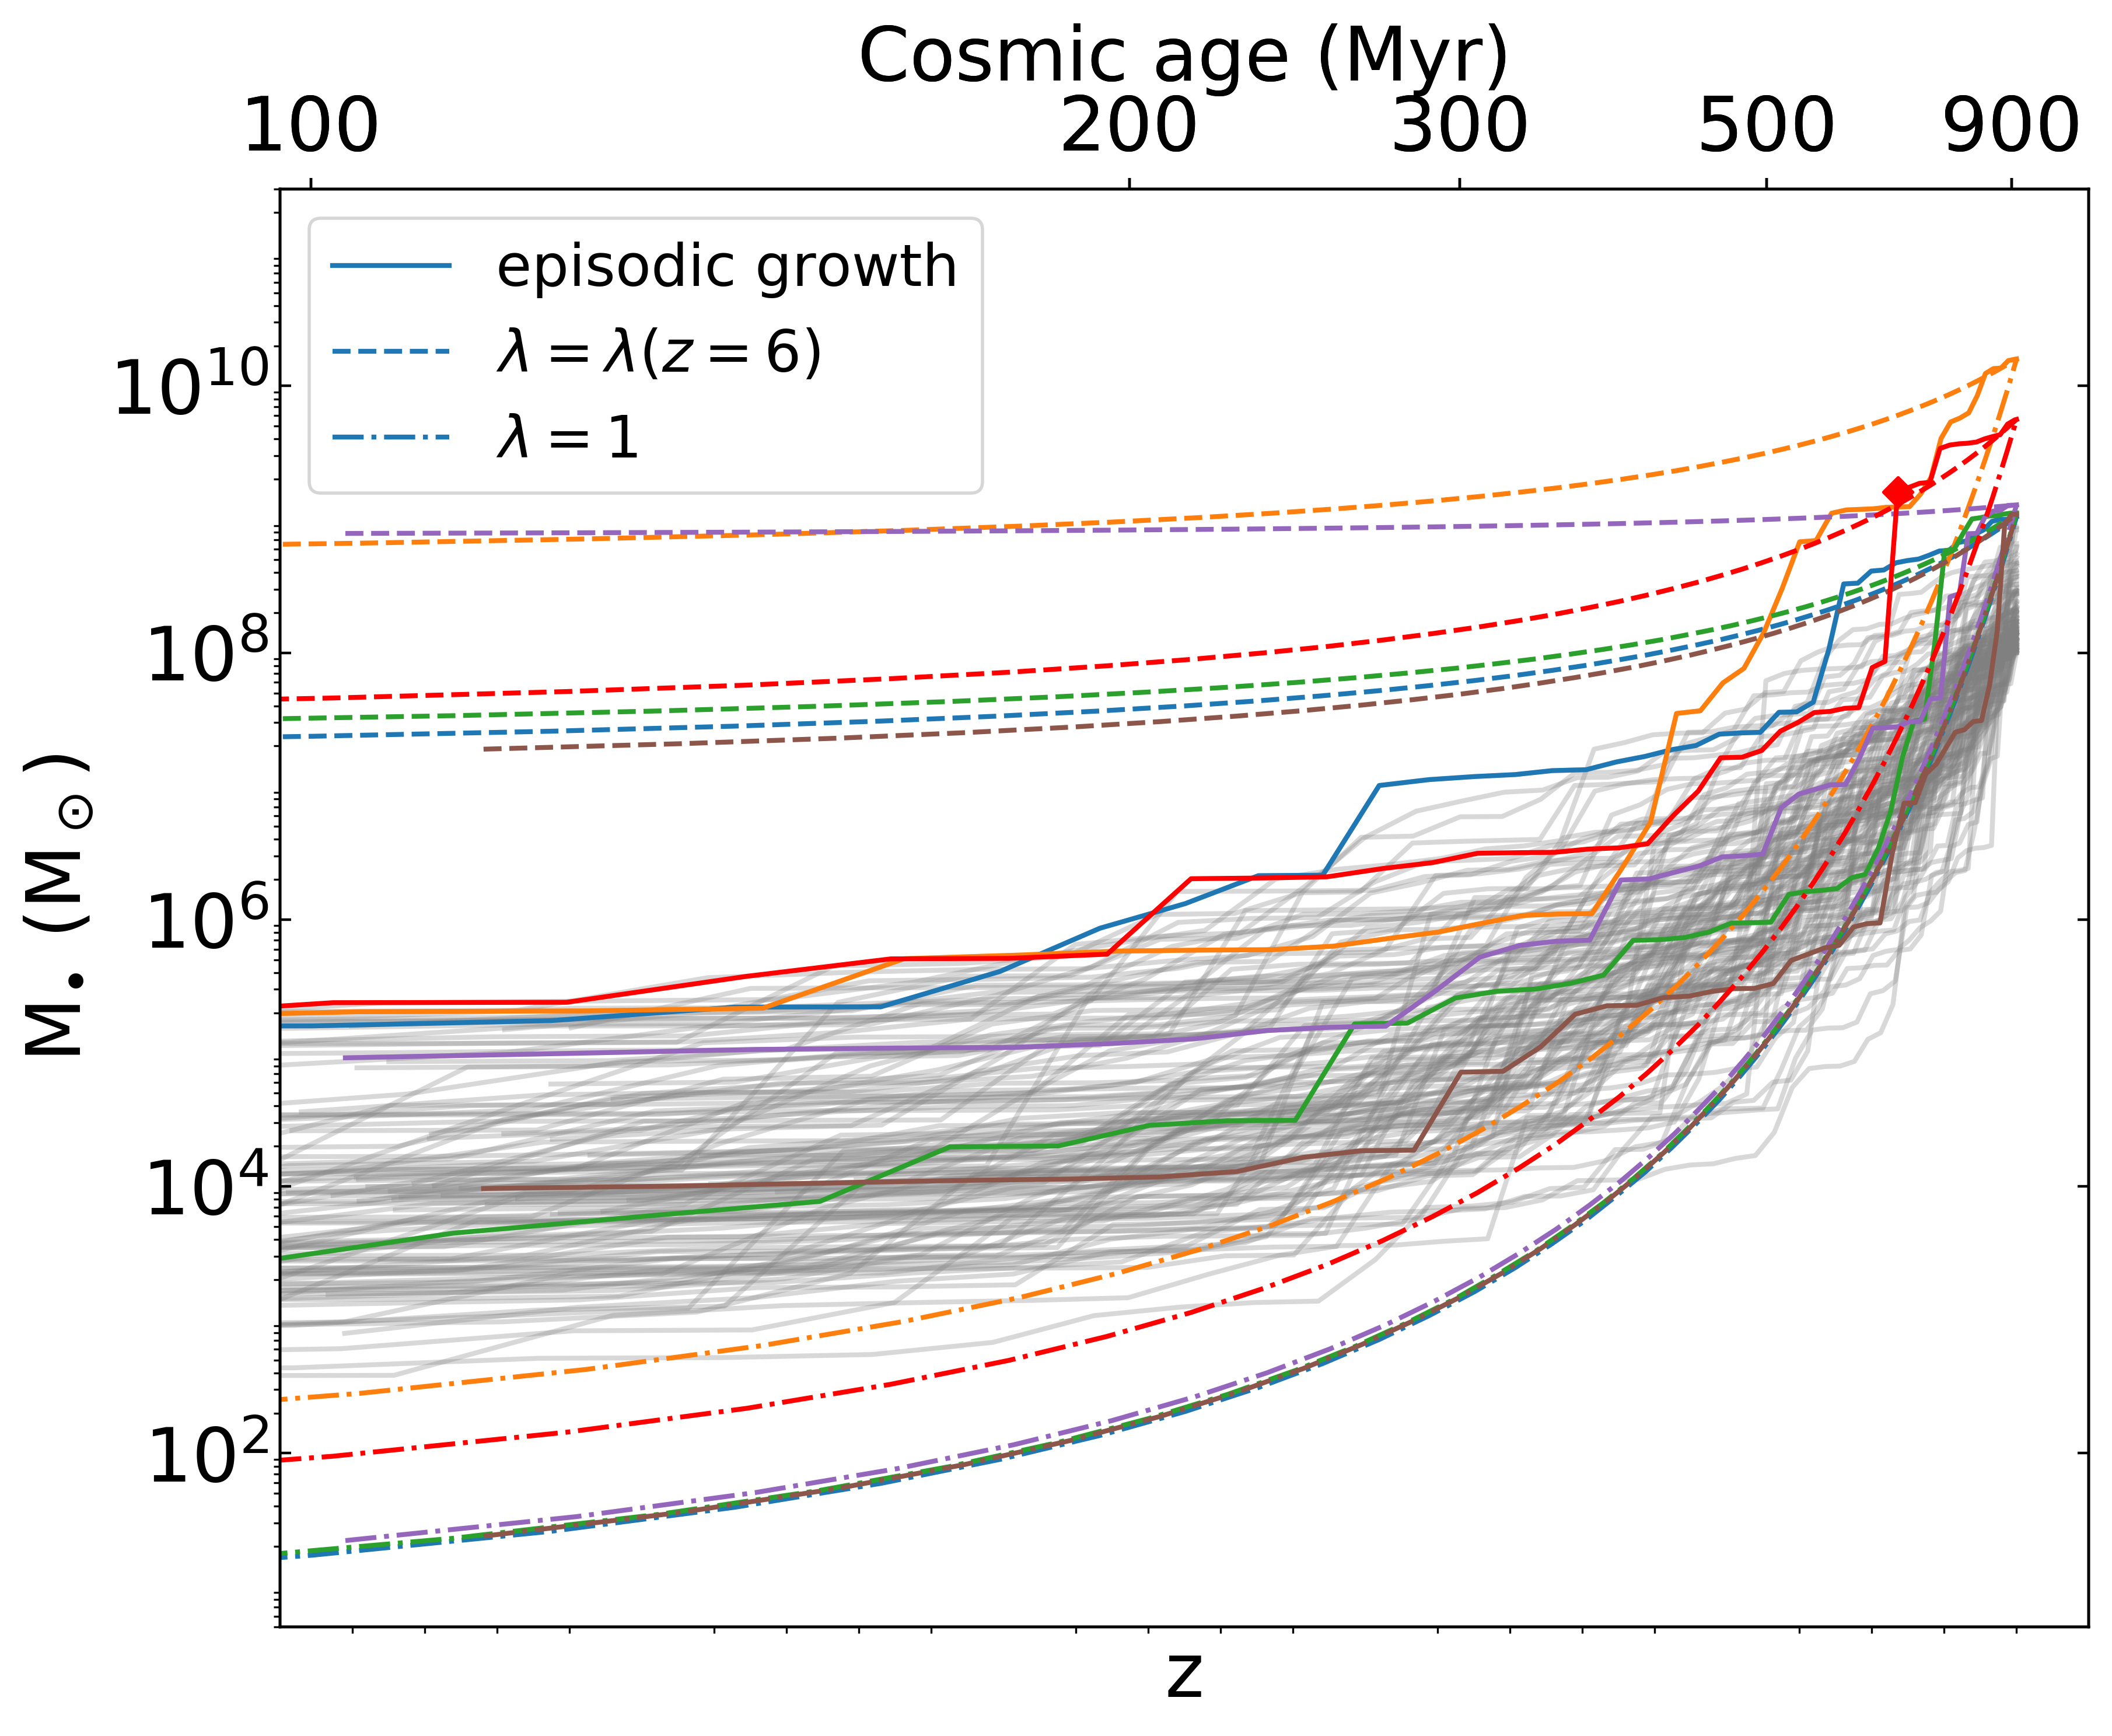
\includegraphics[width=125mm]{Mevol.png}
\caption{
Evolutionary tracks of individual seed BHs with the the best-fit growth model parameters in the $\fseed=0.01$ case.
Among all the samples, we select BHs that reach $M\geq 10^8~\Msun$ at $z=6$ (solid curves). 
The heaviest 7 BHs with $M_\bullet \geq 10^9~\Msun$ at $z=6$ are highlighted with colors. 
For the heaviest BHs, we draw the assembly history assuming an exponential growth with a constant Eddington ratio: 
the $\lambda$-value found at $z=6$ for each BH (dotted curves; extrapolation with an observed value of $\lambda$) and 
$\lambda =1$ (dashed curves; continuous Eddington growth).
%constant $\lambda$ keeping the $z=$ 6 value with dotted lines and 
%Eddington limit growth with $\lambda=1$ with dashed lines.
}
\label{fig:Mevol}
\end{figure*}
%
%


In Fig.~\ref{fig:Mevol}, we show the BH growth tracks that end up with $M_\bullet>10^8~\Msun$ by $z=6$ (grey thin curves).
In this sub-sample, we find five BHs heavier than $M=10^9~\Msun$ (highlighted with colored thick curves),
all of which indicate $\lambda \lesssim 1$ at the  $z=6$ snapshot.
Tracing the BH growth curve back to $z=30$ with the Eddington ratio observed at $z=6$ (dashed curves),
the extrapolated mass of those sub-Eddington BHs at $z=6$ is as massive as $\Mbh \gg 10^6~\Msun$ and is 
substantially higher than the mass range for seed BHs.
%ting BHs trace back to exceedingly massive seeds which are hard to be explained by current seeding scenarios. 
%
%If we extrapolate the BH mass with the $z \sim$ 6 witnessed Eddington ratio back to $z\sim$ 30, 
%the sub-Eddington accreting BHs trace back to exceedingly massive seeds which are hard to be explained by current seeding scenarios. 
It has been pointed out by \cite{2019ApJ...880...77O} that such simple extrapolation of the growth history for low-$\lambda$ quasars 
does not work properly (see their Figure 10).
% In contrast, the extrapolated growth curves of $z\sim$ 6 super-Eddington BHs are unrealistically steep,
% reaching $<100 ~\Msun$ within several hundred million years.
% This fact indicates short durations of the super-Eddington accretion mode.
For comparison, we show the mass growth tracks assuming continuous Eddington accretion (i.e., $\lambda=1$),
where the extrapolated seed mass is $\Mbh \lesssim 10^2~\Msun$ at $z\sim 30$.
%Both treatments of the constant $\lambda$ lead to BH seed masses extrapolation that deviate from the initial seeds we plant. 
% \red{Therefore, one may postulate that short durations of super-Eddington accretion lead to the existence of the massive BHs. KI: what do you mean?}
% \blue{It indicates that super-Eddington accretion episodes are required to explain the existence of the massive BHs.}
Based on the BH seeding and growth model we develop,
we reiterate that multiple accretion episodes with different values of $\lambda$ should be taken into account 
to infer the seeding mass for the observed SMBHs as bright quasars at $z\gtrsim 6-7$,
instead of assuming one single number of the Eddington ratio.




% \red{KI: still not sure what we discuss below... among the 7 BHs, is anyone consistent with Feige's BH?}
\citet{2021ApJ...907L...1W} discovered the currently known most distant quasar at $z=7.642$ (red diamond in Fig.~\ref{fig:Mevol}).
Assuming continuous Eddington accretion, the extrapolated BH is as massive as $10^{4-6}~\Msun$ at $z= 30$. 
%However in our best-fit model, we observe that to trace back BH mass and understand their seeding scenarios, 
%taking constant Eddington ratio derived from high-$z$ observation or assuming $\lambda=1$ are both unrealistic. 
%Therefore we raise a caveat that under these assumptions the seed mass achieved may be unreliable. 
Our best-fit model naturally explains the existence of the most extreme BH,
taking into account the episodical accretion nature of quasars,
%(note extrapolation with the observed $\lambda$ requires an unrealistically high seed mass). 
%including both bursts of accretion and quiescent phases.
%Among the five supermassive BH growth tracks,
%we find one matching this currently known most distant quasar, 
and the consistent growth track among the sub-sample is indicated with the red solid curve 
(with $M_\bullet \simeq 1.7\times 10^9~\Msun$ and $\lambda \simeq 0.6$ at $z=7.6$).
This overmassive growth history is realized by the combination of rare halo environments planting a seed BH 
with $\sim 2\times 10^5~\Msun$ at $z\sim 30$ and several (modest) super-Eddington accretion bursts.


\blue{
Moreover, some individual quasar observations give exceptionally small proximity zone sizes,
indicating short lifetime of their luminous phase $t_{\rm Q} \lesssim 10^4$ yr.
The short quasar lifetime may be due to the young age of quasars ionizing the surrounding IGM \citep[e.g.,][]{2020ApJ...903...60I,2021ApJ...917...38E}.
Our episodic quasar growth model agrees with this argument,
besides alleviates the growth tension of SMBHs by episodic accretion bursts.
In other words, the lifetime of luminous quasar phase is the cumulative time of accreting activity in the current episode.
}



\vspace{2mm}
\subsection{The distribution of the Eddington ratio: \\observed v.s. underlying populations}\label{sec:ldist}

It is challenging to discuss the properties of the underlying quasar population
%Discussion on quasar \textit{intrinsic} properties is naturally difficult, 
because observed quasars are limited by the depths of photometric surveys, not by the BH mass or Eddington ratio.
This unavoidable bias of quasar surveys can be corrected by taking into account the survey completeness;
however, it is still challenging to constrain the low-mass end of the BHMF and low-$\lambda$ end of the ERDF.
%that the surveys are not sensitive to.
In this section, we examine the effect of flux-limited quasar surveys on the observed ERDF, 
taking advantage of our complete sample of high-$z$ BH populations in the whole luminosity range. 


Based on the quasar sample from the best-fit model described in Section~\ref{sec:evol}, 
we select quasars with bolometric luminosity limits $L_{45}=10^{45}~\mathrm{erg~s^{-1}}$ and $L_{46}=10^{46}~\mathrm{erg~s^{-1}}$.
In Fig.~\ref{fig:lhist}, we present the intrinsic ERDFs for the whole BH sample (blue)
and the selected sample with a luminosity cut of $\Lbol \geq L_{45}$ (orange),
and $\Lbol \geq L_{46}$ (green).
For visual comparison, we elevate the observed histograms by a factor of 5 and 30
for the luminosity limits with $L_{45}$ and $L_{46}$, respectively.
The Eddington ratio for the whole sample follows a Schechter shape with a majority of inactive quasars, 
while the observed Eddington ratio is biased toward higher values and the distribution results in a log-normal shape. 
The latter distribution is presented by various observational efforts in the $z\sim$ 6 brightest quasar samples 
\citep[e.g.,][]{2010AJ....140..546W,2019ApJ...873...35S,2021ApJ...923..262Y,2022arXiv220705113F}.
However, our best-fit growth model reproducing both the BHMF and QLF at $z\sim$ 6 suggests the existence of
a large number of underlying BH populations with low Eddington ratios. 
%based on the best-fit growth model connecting the BH seeding and $z\sim$ 6 BHMF and QLF. 
We find that the log-normal shape still holds with the lower luminosity cut, 
%To demonstrate qualitatively the caveat for the detection limit on recovering the intrinsic quasar properties, 
%we also examine the observed ERDF by selecting quasars with $\Lbol>10^{45}~\mathrm{erg~s^{-1}}$. 
but a lower detection limit unveils more hidden quasars with low Eddington ratios. 
Such sub-Eddington BH population at $z>6$ is being probed by the ongoing survey of the Subaru HSC and JWST
\citep{2019ApJ...880...77O,2021jwst.prop.1967O},
and will also be explored by upcoming wide-field surveys such as the Vera C. Rubin Observatory, Euclid, and RST.
% This will be proved by the ongoing observations with the Subaru HSC providing low-luminosity and less-massive BH samples
% (Onoue et al. in prep) and upcoming optical survey by the Vera C. Rubin Observatory.
%Therefore, we emphasize that it is imperative to lower the detection limit in order to 
%understand a more complete quasar sample at high-$z$, 
%so that the numerous dimly accreting BHs can be shed light on.



%%%%%%%
%    Fig. 10
%%%%%%%
\begin{figure}
\centering
% \includegraphics[width=70mm]{distf2N5_06231122_l_hist.png}
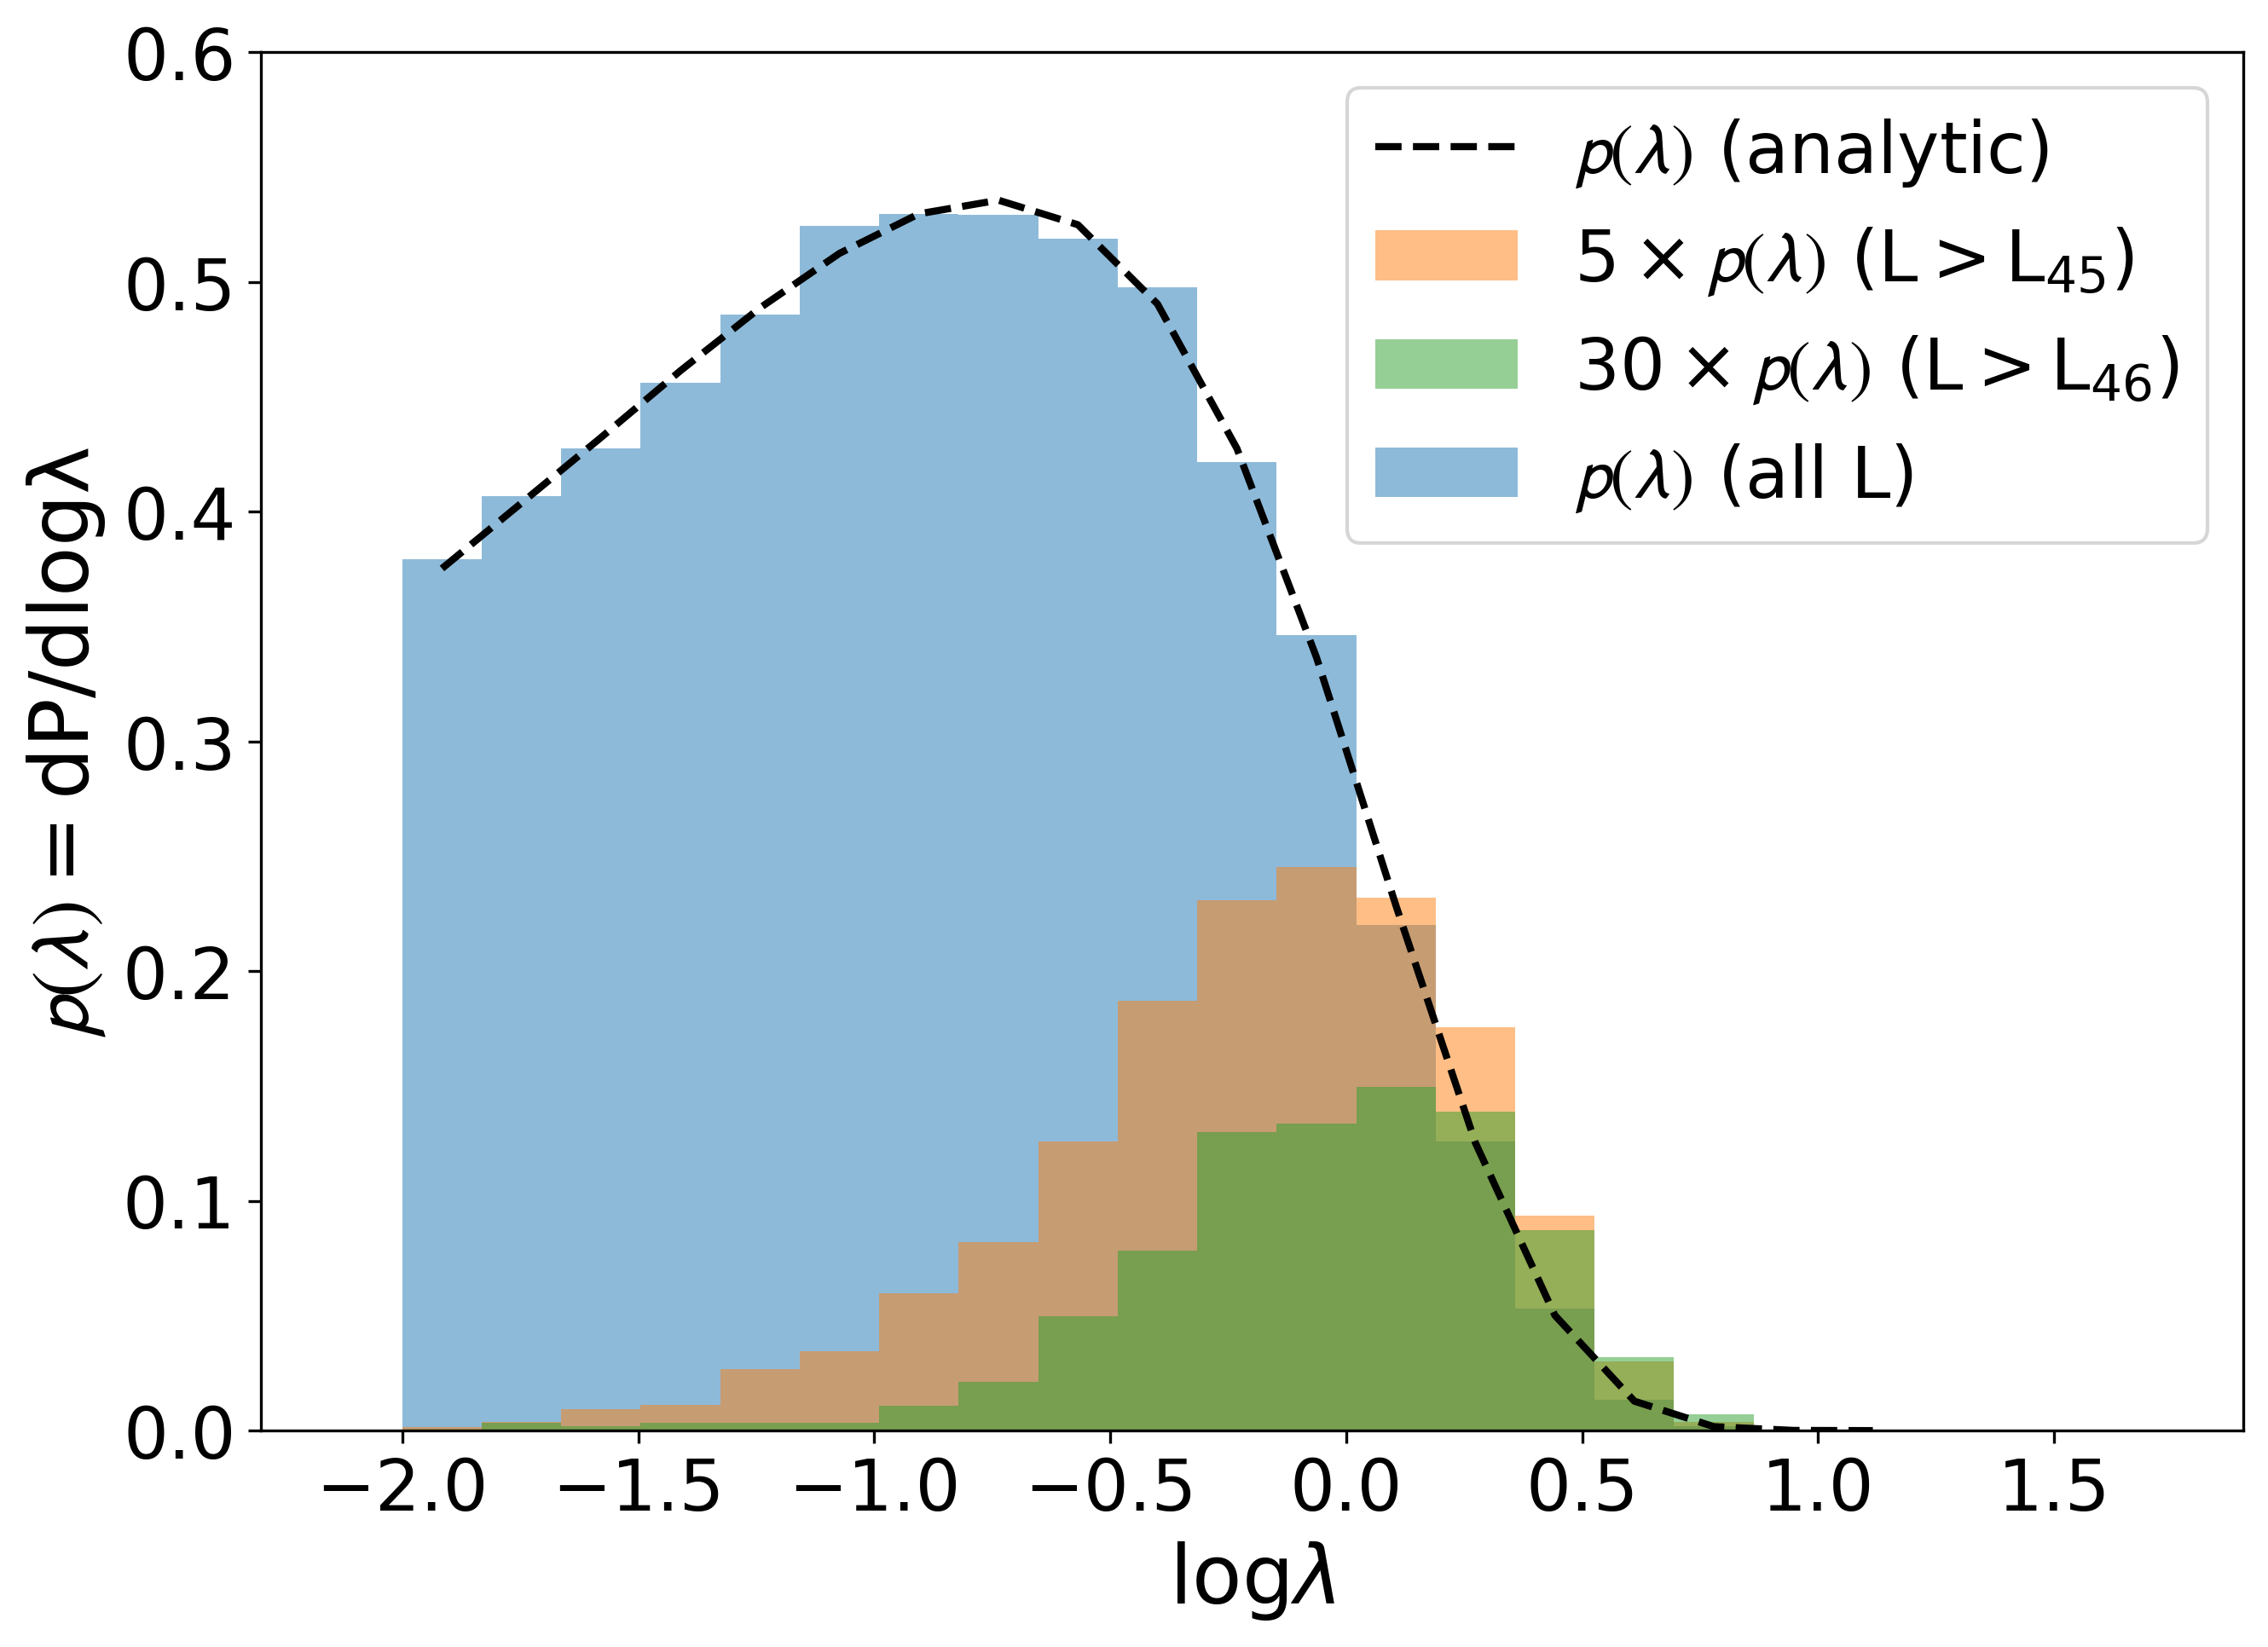
\includegraphics[width=80mm]{l_hist.png}
\caption{
The intrinsic Eddington ratio distribution function for the whole BH sample (blue) and the selected sample with
a luminosity cut of $\Lbol \geq 10^{45}~\mathrm{erg~s^{-1}}$ (orange) and $\Lbol \geq 10^{46}~\mathrm{erg~s^{-1}}$ (green).  
%Intrinsic ERDF (blue) and the observed ones after imposing selection effects by $\Lbol>L_\mathrm{lim}=10^{45}$ (orange) and 10$^{46}$ erg~s$^{-1}$ (green).
The observed histograms are elevated by a factor of 5 and 30, for comparison of the distribution shapes.
The intrinsic ERDF follows the best-fitted Schechter function (dashed curve), 
while the observed ERDF with a detection limit imposed results in a log-normal shape, 
with a large number of sub-Eddington quasars excluded.
The log-normal shape still holds with the lower luminosity cut, 
but a lower detection limit alleviates the selection effect against the low Eddington ratio quasar populations.
%With decreasing $L_\mathrm{lim}$, more low $\lambda$ population is unveiled.
}
\label{fig:lhist}
\end{figure}
  


\section{Summary}
\label{sec:sum}
In this paper, we propose a theoretical model for the redshift-dependent QLF and BHMF at $z\gtrsim 6$,
applying the mass distribution function of seed BHs over $10^2 \lesssim M_\bullet/\Msun \lesssim 10^{5}$
that originate from massive primordial stars formed in the overdense region of the universe.
In our accretion model, those early BH populations are assumed to experience multiple accretion bursts, in each of which a constant Eddington ratio
is assigned following a Schechter distribution function.
We further conduct the MCMC fitting to optimize the BH growth parameters
so that the observed QLF and BHMF at $z\simeq 6$ are simultaneously reproduced. 
Our major findings are summarized as follows.


\begin{itemize}
\item
Our best-fit model to reproduce the QLF and BHMF at $z\simeq 6$ suggests that each accretion burst
lasts $\tau \simeq 20-30$ Myr, which is a fraction of the $e$-folding time for the exponential BH mass growth.
%Our model favors the BH Eddington ratio $\lambda$ following a Schechter distribution function to reproduce the QLF and BHMF at $z\simeq 6$.
%The distribution shape is motivated by low-$z$ AGN observations.
The Schechter shape of the ERDF is characterized with two parameters of 
%The characteristic Eddington ratio $\lambda_0$ and the power law slope $\alpha$ at low Eddington ratio are best-fitted by
$(\lambda_0, \alpha)=(0.89,0.12)$ and $(0.87,0.20)$ for the BH seeding fraction of $\fseed = 0.01$ and $0.1$, respectively.
%The parameter $\tau$ characterizing the duration of each accretion burst is featured by our model,
%with typical values $\tau \simeq 20-30$ Myr.
%For longer (and shorter) burst durations, the number of BHs at the high mass end is over(-under) produced.
Multiple accretion bursts with variable Eddington ratios enable the early BH population to grow and shine,
in a consistent way with the observed QLF and BHMF.


\item
Using the best-fit model parameters, we construct the redshift-dependent QLF and BHMF at $6\leq z \leq 10$.
%\blue{
The two distribution functions suggest a rapid decay of the number and mass density of massive BHs 
and luminous quasars toward higher redshifts, as discussed in previous observations and theoretical studies.
We quantify the decay speed of quasar numbers characterized with a functional form of $\propto 10^{k_{\rm L} z}$,
and find $k_{\rm L}\simeq -0.91$ and $-0.62s$ for the brightest and faintest population at $z>6$.
%with the more luminous quasars decreasing more rapidly toward higher $z$.
%}

\item
Compared to the galaxy luminosity functions at redshifts from $z=7$ to $z\gtrsim 10$,
the QLFs we predict are burried in the faint end at $\Muv \gtrsim -23$ mag,
which makes it challenging to select such faint quasars.
The number of quasars dominates over that of galaxies in the bright end of the UV luminosity function.
We predict the critical magnitude at which galaxies and quasars equally contribute in number,
depending on extrapolation of the galaxy luminosity functions.


\item
We further explore individual BH evolutionary tracks starting from the BH seeds, applying the BH growth model
with the best-fit parameters to examine their statistical properties.
For massive BHs that reach $\gtrsim 10^8~\Msun$ by $z\simeq 6$, the average duty cycle of super-Eddington accretion is as high as $\simeq 15~\%$.
Since the duty cycle is nearly twice that of the entire population, the BH samples observed in $z\simeq 6$ quasars are
biased toward a population that undergoes active accretion episodes.
Multiple accretion-burst treatment well produces the mass assembly history of individual high-$z$ luminous quasars,
unlike the case where one single value of the Eddington ratio is assigned.
We also find that the observed Eddington-ratio distribution function is skewed to a log-normal shape from the intrinsic Schechter function
owing to detection limits of quasar surveys.
Those results will be tested by future deep and wide surveys with the JWST, RST, and Euclid.
\end{itemize}

\acknowledgments
We greatly thank Jin Wu, Zhiwei Pan, BBB, and CCC for constructive discussions. 
We acknowledge support from the National Natural Science Foundation of China 
(12073003, 12003003, 11721303, 11991052, 11950410493, 1215041030, and 12150410307), 
and the China Manned Space Project Nos. CMS-CSST-2021-A04 and CMS-CSST-2021-A06. 
The numerical simulations were performed with the Cray XC50 at the Center for Computational Astrophysics (CfCA) 
of the National Astronomical Observatory of Japan and with the High-performance Computing Platform of Peking University.
%% To help institutions obtain information on the effectiveness of their 
%% telescopes the AAS Journals has created a group of keywords for telescope 
%% facilities.
%
%% Following the acknowledgments section, use the following syntax and the
%% \facility{} or \facilities{} macros to list the keywords of facilities used 
%% in the research for the paper.  Each keyword is check against the master 
%% list during copy editing.  Individual instruments can be provided in 
%% parentheses, after the keyword, but they are not verified.


% \facilities{HST(STIS), Swift(XRT and UVOT), AAVSO, CTIO:1.3m, CTIO:1.5m,CXO}

%% Similar to \facility{}, there is the optional \software command to allow 
%% authors a place to specify which programs were used during the creation of 
%% the manuscript. Authors should list each code and include either a
%% citation or url to the code inside ()s when available.

% \software{astropy \citep{2013A&A...558A..33A,2018AJ....156..123A},  
%           Cloudy \citep{2013RMxAA..49..137F}, 
%           Source Extractor \citep{1996A&AS..117..393B}
%           }

%% Appendix material should be preceded with a single \appendix command.
%% There should be a \section command for each appendix. Mark appendix
%% subsections with the same markup you use in the main body of the paper.

%% Each Appendix (indicated with \section) will be lettered A, B, C, etc.
%% The equation counter will reset when it encounters the \appendix
%% command and will number appendix equations (A1), (A2), etc. The
%% Figure and Table counter will not reset.

%% For this sample we use BibTeX plus aasjournals.bst to generate the
%% the bibliography. The sample631.bib file was populated from ADS. To
%% get the citations to show in the compiled file do the following:
%%
%% pdflatex sample631.tex
%% bibtext sample631
%% pdflatex sample631.tex
%% pdflatex sample631.tex

\appendix


%%%%%%%
%    Fig. 11
%%%%%%%
\begin{figure*}
\centering
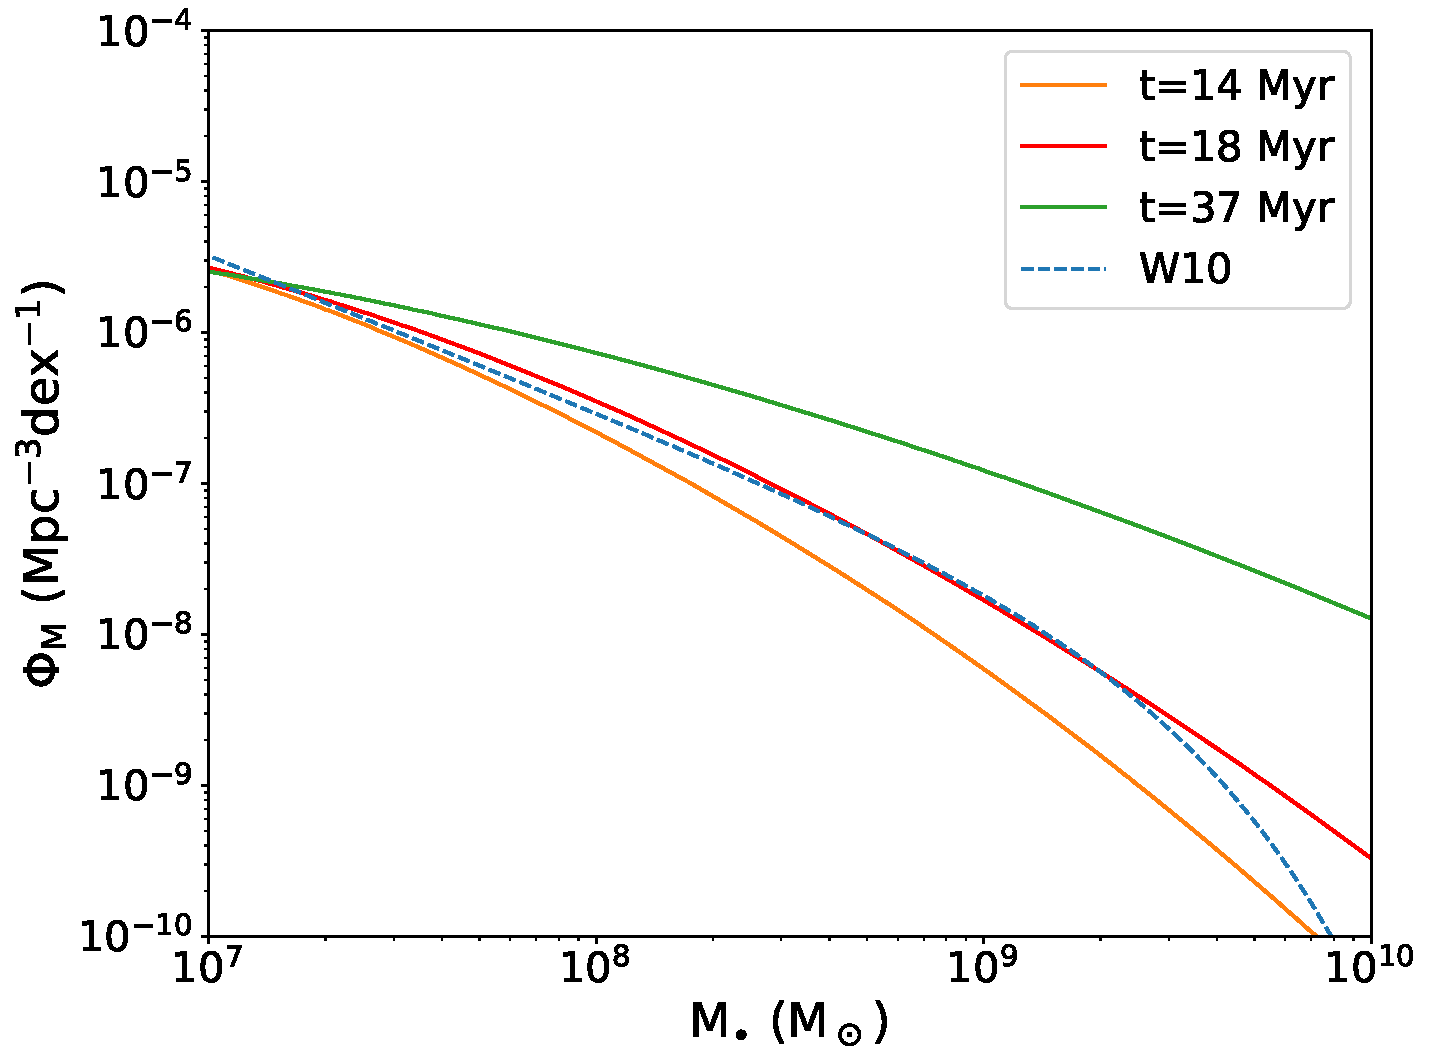
\includegraphics[width=80mm]{f2MFtau.pdf}
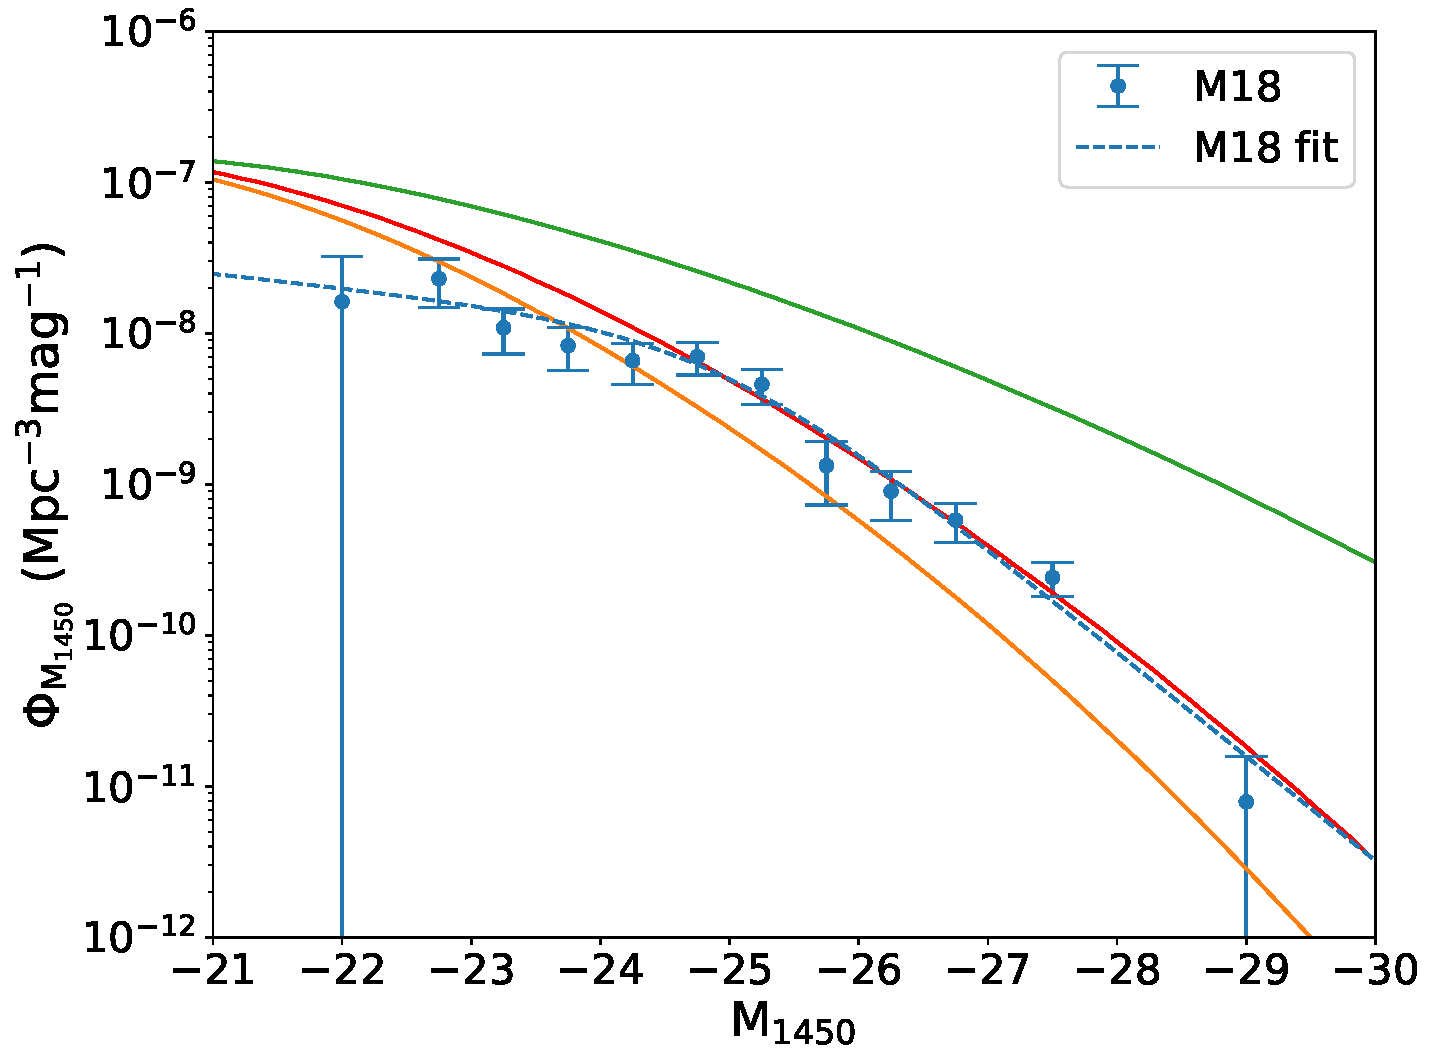
\includegraphics[width=80mm]{f2LFtau.pdf}
\caption{
The BH mass function (left) and quasar luminosity function (right) at $z=$ 6 in the case of $\fseed=0.01$, 
with different values of $\tlife=$ 10, 18 (the best-fit value), and 50 Myr, respectively.
Note that the other parameters are fixed to the best-fit values. 
The $z=6$ BHMF (\citetalias{2010AJ....140..546W}) and QLF (\citetalias{2018ApJ...869..150M}) 
are overlaid with the blue curve and data points.
With shorter (longer) timescales of each accretion episode $\tlife$, the number of BHs at the high mass end and bright end is under(over)-produced.
%Right panel: QLF at $z=$ 6 calculated with the same parameters as in the left panel.
%The overlaid blue dots are from the \citetalias{2018ApJ...869..150M} $z\sim$ 6 quasar observation. 
%With $\tlife$ values different from the best-fit value, the consequent QLF show 
%similar trends of deviation from observation as in the BHMF curves.
Multiple accretion bursts in each duration of $\tau \simeq 20$ Myr best produce the observations,
which is nearly half of the $e$-folding time of the exponential BH mass growth.
}
\label{fig:tau}
%\vspace{4mm}
\end{figure*}

\vspace{2mm}
\section{Model dependence}\label{sec:modep}
As described in Section~\ref{sec:model}, we introduce the parameter $\tau$ as a typical timescale
for individual durations of quasar accretion activity.
Specifically, we assign an Eddington ratio $\lambda$ following the ERDF for all BHs in each cycle
with a time duration of $\tau$.
Variable accretion episodes in every cycle essentially modify the effective ERDF in the whole BH growth history,
because multiple sampling of $\lambda$ reduces the possibility of a BH growing with $\lambda \gtrsim \lambda_0$
compared to that with a single sampling of $\lambda$.
%However at any time during growth, the ERDF of the BH population remains the same as at $z\sim$ 6,
%therefore we ensure treating all cosmic time equally.
In what follows, we demonstrate the role of $\tlife$ in shaping the BHMF evolution and the consequent QLF.
% tau极端小,则非常小的lambda,不能解释 (且delta func? 有必要说或是放在后面讨论?)

In the left panel of Fig.~\ref{fig:tau}, we present the BHMF at $z=6$ for three different values of $\tlife=14$, $18$, and $37$ Myr,
but keeping the other parameters to the best-fit values ($\lambda_0=0.87$ and $\alpha=0.20$) for the case with $\fseed=0.01$.
We note that $\tlife \approx$ 18 Myr is the best-fit value reproducing the BHMF consistent with that of \citetalias{2010AJ....140..546W},
and the other two values represent the $16$ and $84$ percentiles of the one-dimensional distribution of $\tau$, respectively (see Fig.~\ref{fig:contour}).
%the other two cases demonstrate the sensitivity of the $\tlife$ value in producing the bulk of massive BHs
%and the slope in the high mass tail.
For $\tlife=14$ Myr, the frequency of Eddington ratio assignment increases by a factor of 1.3 until $z=6$.
%to $\sim$ 80 from $\sim$ 40 with the best-fit $\tlife$ value.
Therefore, continuous and efficient growth of BHs with $\lambda \gtrsim \lambda_0$ is less likely to occur,
%high Eddington ratio accretion along the growth is lower,
suppressing the formation of BHs heavier than $M_\bullet \simeq 10^8~\Msun$.
Moreover, if a high Eddington ratio is given with a certain but low probability, the BH mass hardly increases
within $\tlife=14$ Myr, which is $\simeq 30\%$ of the $e$-folding timescale.
On the other hand, for $\tlife=$ 37 Myr, there is a non-negligible probability that
% $\sim$ 16 times of Eddington ratio assignment,
more BHs experience high accretion rates with $\lambda\gtrsim \lambda_0$ through their assembly history.
%high values of $\lambda\gtrsim \lambda_0$ is non-negligibly realized in the BHMF evolution.
Therefore, the high mass end of the BHMF is further enhanced and those massive populations are substantially
overproduced compared to the observed abundance.
%in the high mass end of BHMF at $z=$ 6, the BH population is significantly overproduced than the constraints from observation.

The QLF at $z=6$ is shown in the right panel of Fig.~\ref{fig:tau}.
%In the conversion from BHMF to QLF, the ERDF is the same for different $\tlife$ values,
%following the $P(\lambda)$ in Eq.~(\ref{eq:Pl}) with $\lambda_0=0.87$ and $\alpha=0.20$.
Overall, the dependence of the QLF on the choice of $\tau$ shows the same trend as in the BHMF,
%the deviation from the observed QLF of \citetalias{2018ApJ...869..150M} shows similar trends as in the BHMF.
i.e., higher (lower) $\tlife$ values lead to under(over)-production of the luminous quasar population.
The best-fit value of $\tlife (\simeq 18$ Myr) favors a moderate fraction of $t_{\rm S}$.
This result demonstrates the importance of early BHs experiencing multiple accretion episodes to 
reproduce the observed distributions of BH mass and luminosity of quasars at $z\sim$ 6.
% In \S\ref{sec:evol}, we apply this episodic accretion model to individual growth pathways of high-$z$ quasars
% and demonstrate that normal seeding mechanisms can explain the existence of massive BHs with low luminosity
% observed at $z\simeq 6-7$.




% \clearpage

% \newpage

\vspace{100mm}
\bibliography{ref}{}
\bibliographystyle{aasjournal}

%% This command is needed to show the entire author+affiliation list when
%% the collaboration and author truncation commands are used.  It has to
%% go at the end of the manuscript.
%\allauthors

%% Include this line if you are using the \added, \replaced, \deleted
%% commands to see a summary list of all changes at the end of the article.
%\listofchanges

\end{CJK*}
\end{document}

% End of file `sample631.tex'.
